% Options for packages loaded elsewhere
\PassOptionsToPackage{unicode}{hyperref}
\PassOptionsToPackage{hyphens}{url}
%
\documentclass[
]{book}
\usepackage{amsmath,amssymb}
\usepackage{iftex}
\ifPDFTeX
  \usepackage[T1]{fontenc}
  \usepackage[utf8]{inputenc}
  \usepackage{textcomp} % provide euro and other symbols
\else % if luatex or xetex
  \usepackage{unicode-math} % this also loads fontspec
  \defaultfontfeatures{Scale=MatchLowercase}
  \defaultfontfeatures[\rmfamily]{Ligatures=TeX,Scale=1}
\fi
\usepackage{lmodern}
\ifPDFTeX\else
  % xetex/luatex font selection
\fi
% Use upquote if available, for straight quotes in verbatim environments
\IfFileExists{upquote.sty}{\usepackage{upquote}}{}
\IfFileExists{microtype.sty}{% use microtype if available
  \usepackage[]{microtype}
  \UseMicrotypeSet[protrusion]{basicmath} % disable protrusion for tt fonts
}{}
\makeatletter
\@ifundefined{KOMAClassName}{% if non-KOMA class
  \IfFileExists{parskip.sty}{%
    \usepackage{parskip}
  }{% else
    \setlength{\parindent}{0pt}
    \setlength{\parskip}{6pt plus 2pt minus 1pt}}
}{% if KOMA class
  \KOMAoptions{parskip=half}}
\makeatother
\usepackage{xcolor}
\usepackage{color}
\usepackage{fancyvrb}
\newcommand{\VerbBar}{|}
\newcommand{\VERB}{\Verb[commandchars=\\\{\}]}
\DefineVerbatimEnvironment{Highlighting}{Verbatim}{commandchars=\\\{\}}
% Add ',fontsize=\small' for more characters per line
\usepackage{framed}
\definecolor{shadecolor}{RGB}{248,248,248}
\newenvironment{Shaded}{\begin{snugshade}}{\end{snugshade}}
\newcommand{\AlertTok}[1]{\textcolor[rgb]{0.94,0.16,0.16}{#1}}
\newcommand{\AnnotationTok}[1]{\textcolor[rgb]{0.56,0.35,0.01}{\textbf{\textit{#1}}}}
\newcommand{\AttributeTok}[1]{\textcolor[rgb]{0.13,0.29,0.53}{#1}}
\newcommand{\BaseNTok}[1]{\textcolor[rgb]{0.00,0.00,0.81}{#1}}
\newcommand{\BuiltInTok}[1]{#1}
\newcommand{\CharTok}[1]{\textcolor[rgb]{0.31,0.60,0.02}{#1}}
\newcommand{\CommentTok}[1]{\textcolor[rgb]{0.56,0.35,0.01}{\textit{#1}}}
\newcommand{\CommentVarTok}[1]{\textcolor[rgb]{0.56,0.35,0.01}{\textbf{\textit{#1}}}}
\newcommand{\ConstantTok}[1]{\textcolor[rgb]{0.56,0.35,0.01}{#1}}
\newcommand{\ControlFlowTok}[1]{\textcolor[rgb]{0.13,0.29,0.53}{\textbf{#1}}}
\newcommand{\DataTypeTok}[1]{\textcolor[rgb]{0.13,0.29,0.53}{#1}}
\newcommand{\DecValTok}[1]{\textcolor[rgb]{0.00,0.00,0.81}{#1}}
\newcommand{\DocumentationTok}[1]{\textcolor[rgb]{0.56,0.35,0.01}{\textbf{\textit{#1}}}}
\newcommand{\ErrorTok}[1]{\textcolor[rgb]{0.64,0.00,0.00}{\textbf{#1}}}
\newcommand{\ExtensionTok}[1]{#1}
\newcommand{\FloatTok}[1]{\textcolor[rgb]{0.00,0.00,0.81}{#1}}
\newcommand{\FunctionTok}[1]{\textcolor[rgb]{0.13,0.29,0.53}{\textbf{#1}}}
\newcommand{\ImportTok}[1]{#1}
\newcommand{\InformationTok}[1]{\textcolor[rgb]{0.56,0.35,0.01}{\textbf{\textit{#1}}}}
\newcommand{\KeywordTok}[1]{\textcolor[rgb]{0.13,0.29,0.53}{\textbf{#1}}}
\newcommand{\NormalTok}[1]{#1}
\newcommand{\OperatorTok}[1]{\textcolor[rgb]{0.81,0.36,0.00}{\textbf{#1}}}
\newcommand{\OtherTok}[1]{\textcolor[rgb]{0.56,0.35,0.01}{#1}}
\newcommand{\PreprocessorTok}[1]{\textcolor[rgb]{0.56,0.35,0.01}{\textit{#1}}}
\newcommand{\RegionMarkerTok}[1]{#1}
\newcommand{\SpecialCharTok}[1]{\textcolor[rgb]{0.81,0.36,0.00}{\textbf{#1}}}
\newcommand{\SpecialStringTok}[1]{\textcolor[rgb]{0.31,0.60,0.02}{#1}}
\newcommand{\StringTok}[1]{\textcolor[rgb]{0.31,0.60,0.02}{#1}}
\newcommand{\VariableTok}[1]{\textcolor[rgb]{0.00,0.00,0.00}{#1}}
\newcommand{\VerbatimStringTok}[1]{\textcolor[rgb]{0.31,0.60,0.02}{#1}}
\newcommand{\WarningTok}[1]{\textcolor[rgb]{0.56,0.35,0.01}{\textbf{\textit{#1}}}}
\usepackage{longtable,booktabs,array}
\usepackage{calc} % for calculating minipage widths
% Correct order of tables after \paragraph or \subparagraph
\usepackage{etoolbox}
\makeatletter
\patchcmd\longtable{\par}{\if@noskipsec\mbox{}\fi\par}{}{}
\makeatother
% Allow footnotes in longtable head/foot
\IfFileExists{footnotehyper.sty}{\usepackage{footnotehyper}}{\usepackage{footnote}}
\makesavenoteenv{longtable}
\usepackage{graphicx}
\makeatletter
\def\maxwidth{\ifdim\Gin@nat@width>\linewidth\linewidth\else\Gin@nat@width\fi}
\def\maxheight{\ifdim\Gin@nat@height>\textheight\textheight\else\Gin@nat@height\fi}
\makeatother
% Scale images if necessary, so that they will not overflow the page
% margins by default, and it is still possible to overwrite the defaults
% using explicit options in \includegraphics[width, height, ...]{}
\setkeys{Gin}{width=\maxwidth,height=\maxheight,keepaspectratio}
% Set default figure placement to htbp
\makeatletter
\def\fps@figure{htbp}
\makeatother
\setlength{\emergencystretch}{3em} % prevent overfull lines
\providecommand{\tightlist}{%
  \setlength{\itemsep}{0pt}\setlength{\parskip}{0pt}}
\setcounter{secnumdepth}{5}
\usepackage{booktabs}
\usepackage{amsthm}
\makeatletter
\def\thm@space@setup{%
  \thm@preskip=8pt plus 2pt minus 4pt
  \thm@postskip=\thm@preskip
}
\makeatother
\renewcommand{\chaptername}{Capítulo}
\renewcommand{\contentsname}{Índice}
\ifLuaTeX
  \usepackage{selnolig}  % disable illegal ligatures
\fi
\usepackage[]{natbib}
\bibliographystyle{apalike}
\nocite{*}
\IfFileExists{bookmark.sty}{\usepackage{bookmark}}{\usepackage{hyperref}}
\IfFileExists{xurl.sty}{\usepackage{xurl}}{} % add URL line breaks if available
\urlstyle{same}
\hypersetup{
  pdftitle={Notas de R},
  pdfauthor={Roberto Álvarez},
  hidelinks,
  pdfcreator={LaTeX via pandoc}}

\title{Notas de R}
\author{Roberto Álvarez}
\date{2024-04-17}

\begin{document}
\maketitle

{
\setcounter{tocdepth}{1}
\tableofcontents
}
\hypertarget{notas-de-r-buxe1sico}{%
\chapter{Notas de R básico}\label{notas-de-r-buxe1sico}}

\hypertarget{intro}{%
\chapter{Introducción a R}\label{intro}}

R es un entorno integrado para el manejo de datos, el cálculo, la generación de gráficos y análisis estadísticos. Las principales ventajas del uso de R son:

\begin{enumerate}
\def\labelenumi{\arabic{enumi}.}
\tightlist
\item
  Software libre.
\item
  Facilidad para el manejo y almacenamiento de datos.
\item
  Un conjunto de operadores para el cálculo de vectores y matrices.
\item
  Una colección extensa e integrada de herramientas intermedias para el análisis estadístico de datos.
\item
  Multitud de facilidades gráficas de altísima calidad.
\item
  Un lenguaje de programación (muy) poderoso con muchas librerías especializadas disponibles.
\item
  La mejor herramienta para trabajar con datos genómicos, proteómicos, redes, metabolómica, entre varias más.
\item
  \textbf{Casi todos podemos aprender por nuestra cuenta a usar excel (pero hay que pagar por la licencia, es software privativo\ldots). Sin embargo, es más díficil aprender por nuestra cuenta R; y si lo hacemos nos da una ventaja comparativa sobre el resto.}
\item
  Además excel no es la mejor elección si queremos hacer bioinformática en serio.
\end{enumerate}

\hypertarget{introducciuxf3n-a-r-para-estudiantes-de-microbiologuxeda}{%
\chapter{Introducción a R para Estudiantes de Microbiología}\label{introducciuxf3n-a-r-para-estudiantes-de-microbiologuxeda}}

R es un lenguaje de programación y un entorno de desarrollo estadístico ampliamente utilizado en la comunidad científica, incluida la microbiología. Este poderoso recurso ofrece una variedad de ventajas y funcionalidades que pueden beneficiar significativamente a los estudiantes de microbiología en su investigación y análisis de datos.

\hypertarget{ventajas-de-aprender-r-para-estudiantes-de-microbiologuxeda}{%
\section{Ventajas de Aprender R para Estudiantes de Microbiología}\label{ventajas-de-aprender-r-para-estudiantes-de-microbiologuxeda}}

\hypertarget{anuxe1lisis-estaduxedstico-avanzado}{%
\subsection{1. Análisis Estadístico Avanzado}\label{anuxe1lisis-estaduxedstico-avanzado}}

R proporciona una amplia gama de paquetes y herramientas estadísticas que permiten a los estudiantes de microbiología realizar análisis avanzados de datos, desde pruebas de hipótesis básicas hasta modelos de regresión y análisis multivariados.

\hypertarget{visualizaciuxf3n-de-datos}{%
\subsection{2. Visualización de Datos}\label{visualizaciuxf3n-de-datos}}

Con paquetes como ggplot2, los estudiantes pueden crear visualizaciones de datos interactivas y de alta calidad que facilitan la comprensión de patrones y tendencias en conjuntos de datos microbiológicos, como datos de secuenciación genómica o datos de conteo de microorganismos.

\hypertarget{reproducibilidad-y-documentaciuxf3n}{%
\subsection{3. Reproducibilidad y Documentación}\label{reproducibilidad-y-documentaciuxf3n}}

RMarkdown es una herramienta poderosa que permite a los estudiantes escribir documentos reproducibles que combinan código, resultados y narrativa en un solo lugar. Esto promueve la transparencia, la reproducibilidad y una mejor documentación de los análisis microbiológicos.

\hypertarget{acceso-a-una-comunidad-activa}{%
\subsection{4. Acceso a una Comunidad Activa}\label{acceso-a-una-comunidad-activa}}

R cuenta con una comunidad activa de usuarios y desarrolladores que comparten código, paquetes y recursos educativos. Los estudiantes pueden aprovechar este recurso para buscar ayuda, colaborar en proyectos y mantenerse al tanto de las últimas tendencias en análisis de datos microbiológicos.

\hypertarget{flexibilidad-y-personalizaciuxf3n}{%
\subsection{5. Flexibilidad y Personalización}\label{flexibilidad-y-personalizaciuxf3n}}

R es un lenguaje altamente flexible que permite a los estudiantes adaptar sus análisis a las necesidades específicas de sus proyectos microbiológicos. Desde la manipulación de datos hasta la creación de modelos personalizados, R ofrece la libertad y la capacidad de personalización necesarias para abordar una amplia variedad de preguntas de investigación en microbiología.

Aprender R puede ser extremadamente beneficioso para los estudiantes de microbiología al proporcionarles las herramientas y habilidades necesarias para realizar análisis de datos sofisticados, visualizar resultados de manera efectiva y promover la reproducibilidad en su investigación científica.

\hypertarget{paquetes-o-bibliotecas}{%
\section{Paquetes o bibliotecas}\label{paquetes-o-bibliotecas}}

Las funciones especializadas de R se guardan en paquetes \emph{(packages)} que deben ser invocados ANTES de llamar a una función del paquete.

Una manera de instalar paquetes es mediante el repositorio \href{https://cran.r-project.org/}{CRAN}.

Navega por CRAN y encuentra algunos paquetes que podrían interesarte. Hay miles y cada día aumentan.

Para saber qué paquetes se tienen instalados en
tu máquina teclea la función \texttt{library()}

\begin{Shaded}
\begin{Highlighting}[]
\FunctionTok{library}\NormalTok{()}
\end{Highlighting}
\end{Shaded}

Para cargar un paquete, que se encuentre previamente instalado, se debe teclear
\texttt{library(nombre\_de\_paquete)}

Por ejemplo:

\begin{Shaded}
\begin{Highlighting}[]
\FunctionTok{library}\NormalTok{(gplots)  }
\end{Highlighting}
\end{Shaded}

\begin{verbatim}
## 
## Attaching package: 'gplots'
\end{verbatim}

\begin{verbatim}
## The following object is masked from 'package:stats':
## 
##     lowess
\end{verbatim}

Para visualizar los paquetes ya cargados, teclea:

\begin{Shaded}
\begin{Highlighting}[]
\FunctionTok{search}\NormalTok{()}
\end{Highlighting}
\end{Shaded}

\begin{verbatim}
##  [1] ".GlobalEnv"        "package:gplots"    "tools:rstudio"    
##  [4] "package:stats"     "package:graphics"  "package:grDevices"
##  [7] "package:utils"     "package:datasets"  "package:methods"  
## [10] "Autoloads"         "package:base"
\end{verbatim}

Para visualizar las funciones dentro de un paquete en particular se utiliza:

\begin{Shaded}
\begin{Highlighting}[]
\FunctionTok{ls}\NormalTok{(}\DecValTok{2}\NormalTok{)}
\end{Highlighting}
\end{Shaded}

\begin{verbatim}
##  [1] "angleAxis"      "balloonplot"    "bandplot"       "barplot2"      
##  [5] "bluered"        "boxplot2"       "ci2d"           "col2hex"       
##  [9] "colorpanel"     "greenred"       "heatmap.2"      "hist2d"        
## [13] "lmplot2"        "lowess"         "ooplot"         "overplot"      
## [17] "panel.overplot" "plot.venn"      "plotCI"         "plotLowess"    
## [21] "plotmeans"      "qqnorm.aov"     "redblue"        "redgreen"      
## [25] "reorder.factor" "residplot"      "rich.colors"    "sinkplot"      
## [29] "smartlegend"    "space"          "textplot"       "venn"          
## [33] "wapply"
\end{verbatim}

\textbf{EJEMPLOS DE VISUALIZACIÓN DE GRÁFICOS}

\begin{Shaded}
\begin{Highlighting}[]
\FunctionTok{demo}\NormalTok{(graphics)}
\end{Highlighting}
\end{Shaded}

\begin{verbatim}
## 
## 
##  demo(graphics)
##  ---- ~~~~~~~~
## 
## > #  Copyright (C) 1997-2009 The R Core Team
## > 
## > require(datasets)
## 
## > require(grDevices); require(graphics)
## 
## > ## Here is some code which illustrates some of the differences between
## > ## R and S graphics capabilities.  Note that colors are generally specified
## > ## by a character string name (taken from the X11 rgb.txt file) and that line
## > ## textures are given similarly.  The parameter "bg" sets the background
## > ## parameter for the plot and there is also an "fg" parameter which sets
## > ## the foreground color.
## > 
## > 
## > x <- stats::rnorm(50)
## 
## > opar <- par(bg = "white")
## 
## > plot(x, ann = FALSE, type = "n")
\end{verbatim}

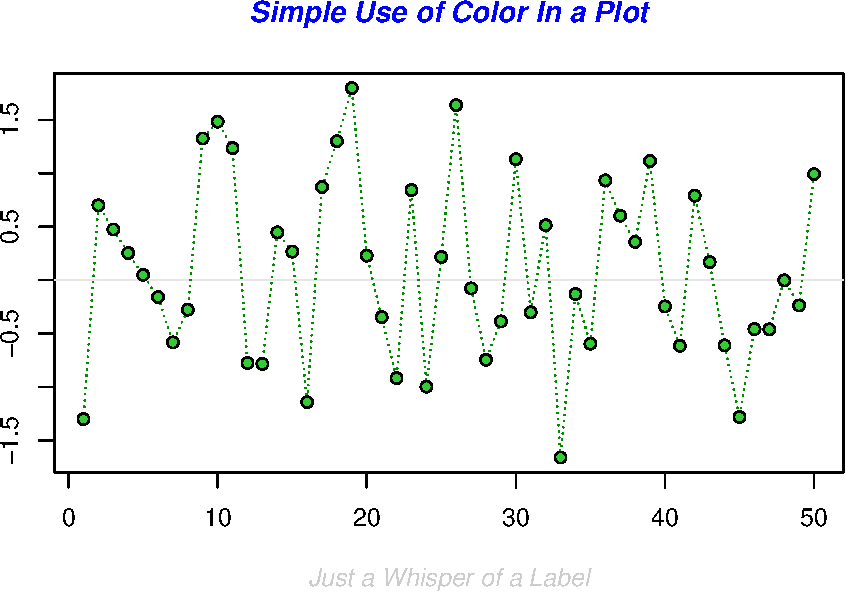
\includegraphics{bookdown-demo_files/figure-latex/unnamed-chunk-5-1.pdf}

\begin{verbatim}
## 
## > abline(h = 0, col = gray(.90))
## 
## > lines(x, col = "green4", lty = "dotted")
## 
## > points(x, bg = "limegreen", pch = 21)
## 
## > title(main = "Simple Use of Color In a Plot",
## +       xlab = "Just a Whisper of a Label",
## +       col.main = "blue", col.lab = gray(.8),
## +       cex.main = 1.2, cex.lab = 1.0, font.main = 4, font.lab = 3)
## 
## > ## A little color wheel.    This code just plots equally spaced hues in
## > ## a pie chart.    If you have a cheap SVGA monitor (like me) you will
## > ## probably find that numerically equispaced does not mean visually
## > ## equispaced.  On my display at home, these colors tend to cluster at
## > ## the RGB primaries.  On the other hand on the SGI Indy at work the
## > ## effect is near perfect.
## > 
## > par(bg = "gray")
## 
## > pie(rep(1,24), col = rainbow(24), radius = 0.9)
\end{verbatim}

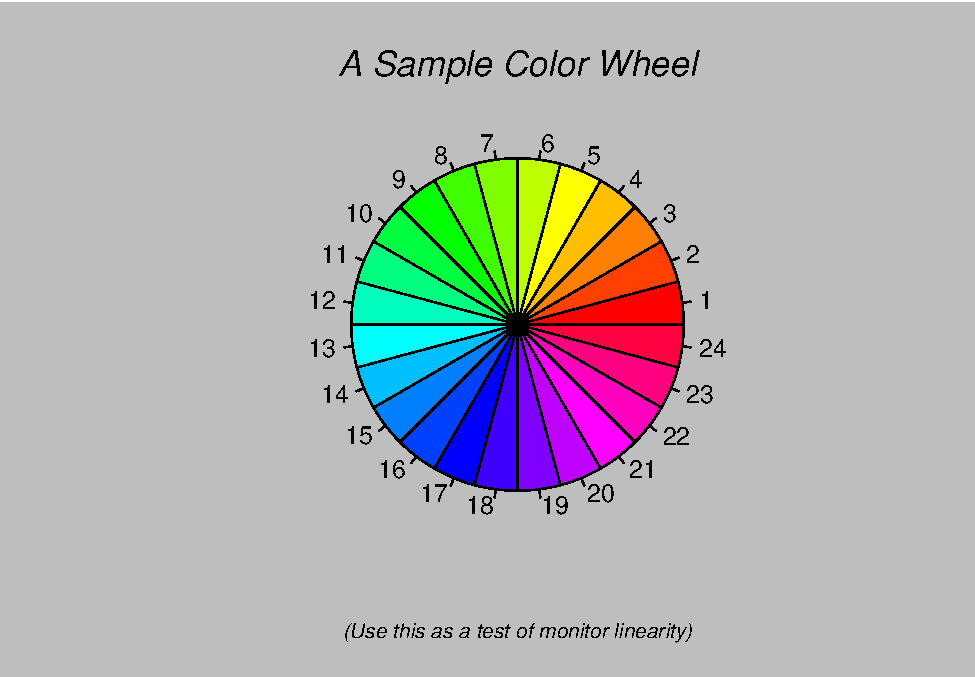
\includegraphics{bookdown-demo_files/figure-latex/unnamed-chunk-5-2.pdf}

\begin{verbatim}
## 
## > title(main = "A Sample Color Wheel", cex.main = 1.4, font.main = 3)
## 
## > title(xlab = "(Use this as a test of monitor linearity)",
## +       cex.lab = 0.8, font.lab = 3)
## 
## > ## We have already confessed to having these.  This is just showing off X11
## > ## color names (and the example (from the postscript manual) is pretty "cute".
## > 
## > pie.sales <- c(0.12, 0.3, 0.26, 0.16, 0.04, 0.12)
## 
## > names(pie.sales) <- c("Blueberry", "Cherry",
## +              "Apple", "Boston Cream", "Other", "Vanilla Cream")
## 
## > pie(pie.sales,
## +     col = c("purple","violetred1","green3","cornsilk","cyan","white"))
\end{verbatim}

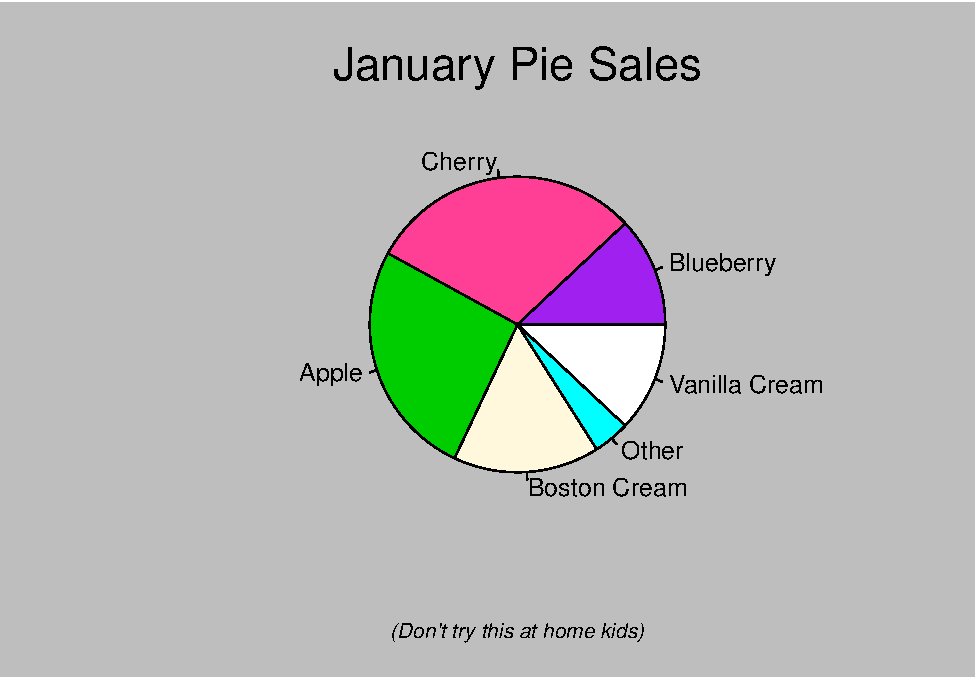
\includegraphics{bookdown-demo_files/figure-latex/unnamed-chunk-5-3.pdf}

\begin{verbatim}
## 
## > title(main = "January Pie Sales", cex.main = 1.8, font.main = 1)
## 
## > title(xlab = "(Don't try this at home kids)", cex.lab = 0.8, font.lab = 3)
## 
## > ## Boxplots:  I couldn't resist the capability for filling the "box".
## > ## The use of color seems like a useful addition, it focuses attention
## > ## on the central bulk of the data.
## > 
## > par(bg="cornsilk")
## 
## > n <- 10
## 
## > g <- gl(n, 100, n*100)
## 
## > x <- rnorm(n*100) + sqrt(as.numeric(g))
## 
## > boxplot(split(x,g), col="lavender", notch=TRUE)
\end{verbatim}

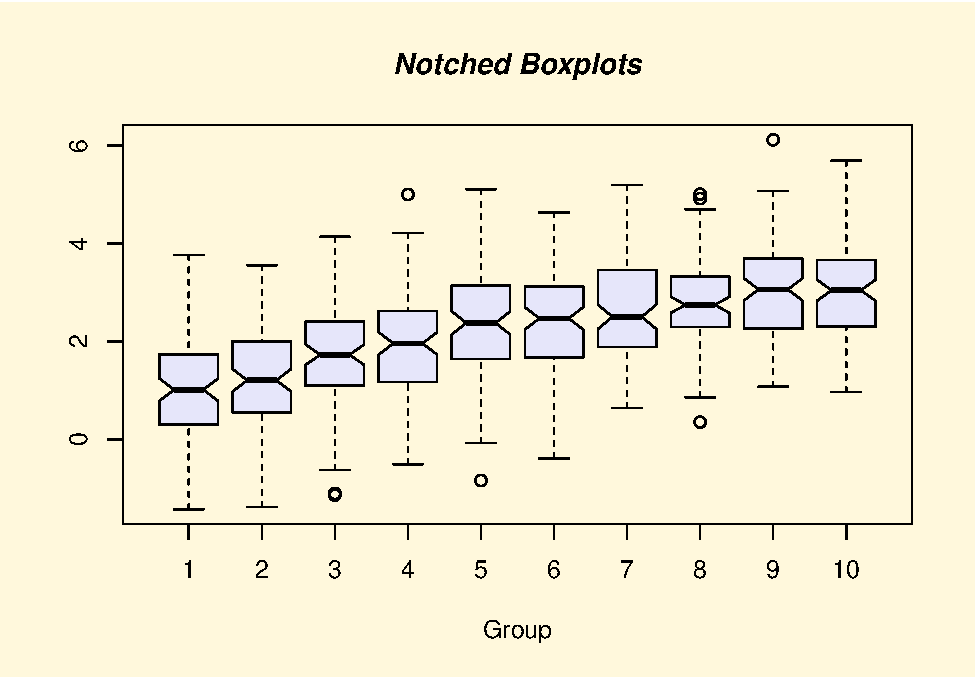
\includegraphics{bookdown-demo_files/figure-latex/unnamed-chunk-5-4.pdf}

\begin{verbatim}
## 
## > title(main="Notched Boxplots", xlab="Group", font.main=4, font.lab=1)
## 
## > ## An example showing how to fill between curves.
## > 
## > par(bg="white")
## 
## > n <- 100
## 
## > x <- c(0,cumsum(rnorm(n)))
## 
## > y <- c(0,cumsum(rnorm(n)))
## 
## > xx <- c(0:n, n:0)
## 
## > yy <- c(x, rev(y))
## 
## > plot(xx, yy, type="n", xlab="Time", ylab="Distance")
\end{verbatim}

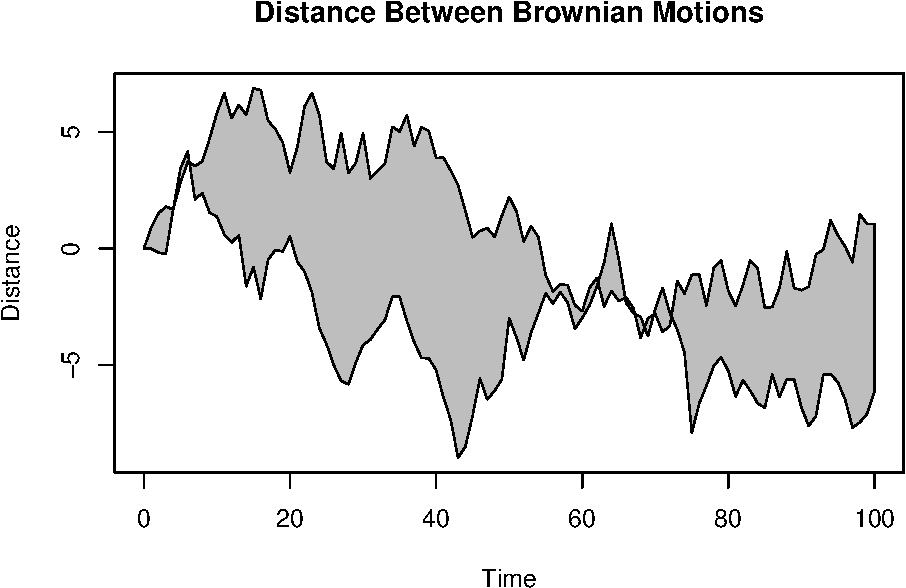
\includegraphics{bookdown-demo_files/figure-latex/unnamed-chunk-5-5.pdf}

\begin{verbatim}
## 
## > polygon(xx, yy, col="gray")
## 
## > title("Distance Between Brownian Motions")
## 
## > ## Colored plot margins, axis labels and titles.    You do need to be
## > ## careful with these kinds of effects.    It's easy to go completely
## > ## over the top and you can end up with your lunch all over the keyboard.
## > ## On the other hand, my market research clients love it.
## > 
## > x <- c(0.00, 0.40, 0.86, 0.85, 0.69, 0.48, 0.54, 1.09, 1.11, 1.73, 2.05, 2.02)
## 
## > par(bg="lightgray")
## 
## > plot(x, type="n", axes=FALSE, ann=FALSE)
\end{verbatim}

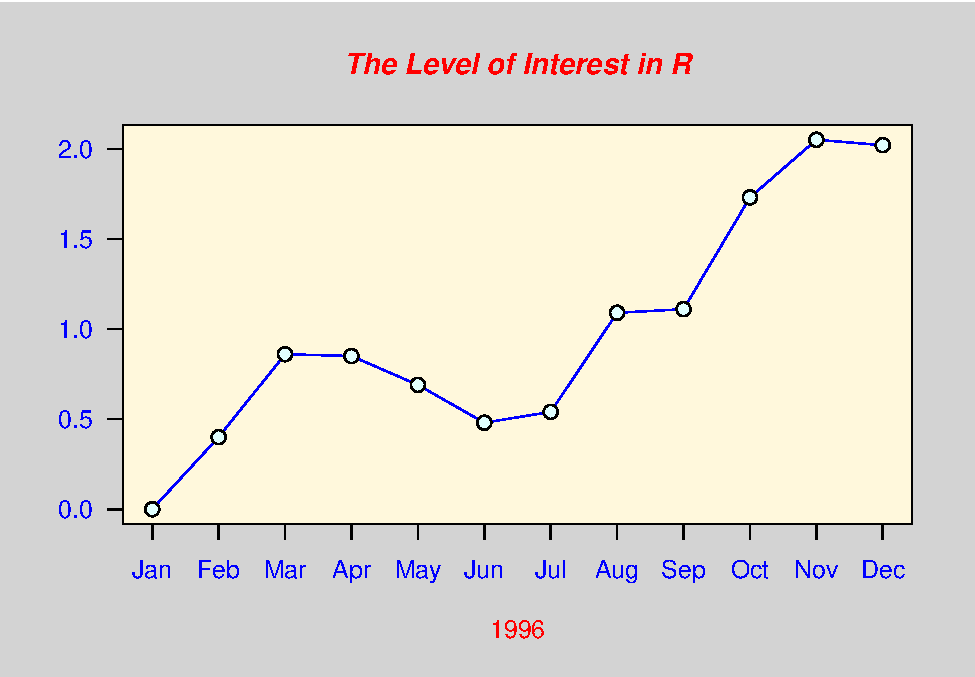
\includegraphics{bookdown-demo_files/figure-latex/unnamed-chunk-5-6.pdf}

\begin{verbatim}
## 
## > usr <- par("usr")
## 
## > rect(usr[1], usr[3], usr[2], usr[4], col="cornsilk", border="black")
## 
## > lines(x, col="blue")
## 
## > points(x, pch=21, bg="lightcyan", cex=1.25)
## 
## > axis(2, col.axis="blue", las=1)
## 
## > axis(1, at=1:12, lab=month.abb, col.axis="blue")
## 
## > box()
## 
## > title(main= "The Level of Interest in R", font.main=4, col.main="red")
## 
## > title(xlab= "1996", col.lab="red")
## 
## > ## A filled histogram, showing how to change the font used for the
## > ## main title without changing the other annotation.
## > 
## > par(bg="cornsilk")
## 
## > x <- rnorm(1000)
## 
## > hist(x, xlim=range(-4, 4, x), col="lavender", main="")
\end{verbatim}

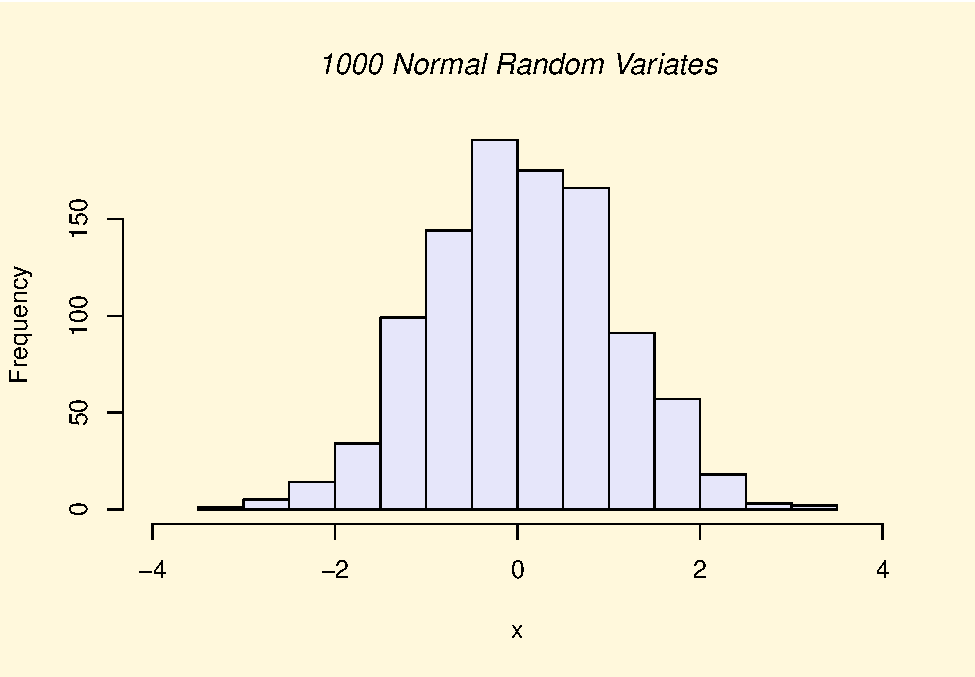
\includegraphics{bookdown-demo_files/figure-latex/unnamed-chunk-5-7.pdf}

\begin{verbatim}
## 
## > title(main="1000 Normal Random Variates", font.main=3)
## 
## > ## A scatterplot matrix
## > ## The good old Iris data (yet again)
## > 
## > pairs(iris[1:4], main="Edgar Anderson's Iris Data", font.main=4, pch=19)
\end{verbatim}

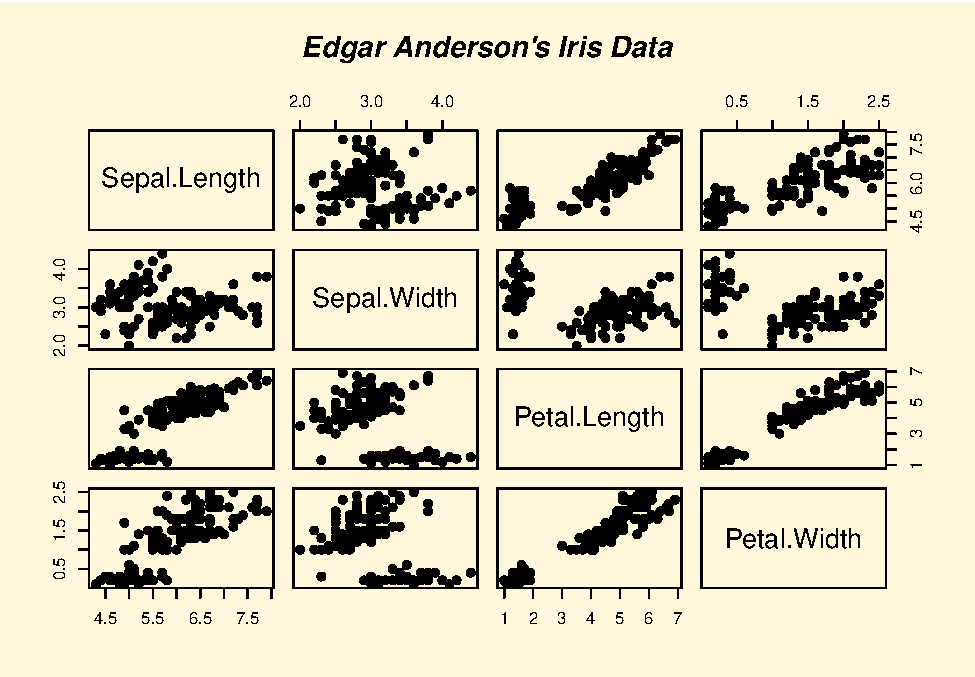
\includegraphics{bookdown-demo_files/figure-latex/unnamed-chunk-5-8.pdf}

\begin{verbatim}
## 
## > pairs(iris[1:4], main="Edgar Anderson's Iris Data", pch=21,
## +       bg = c("red", "green3", "blue")[unclass(iris$Species)])
\end{verbatim}

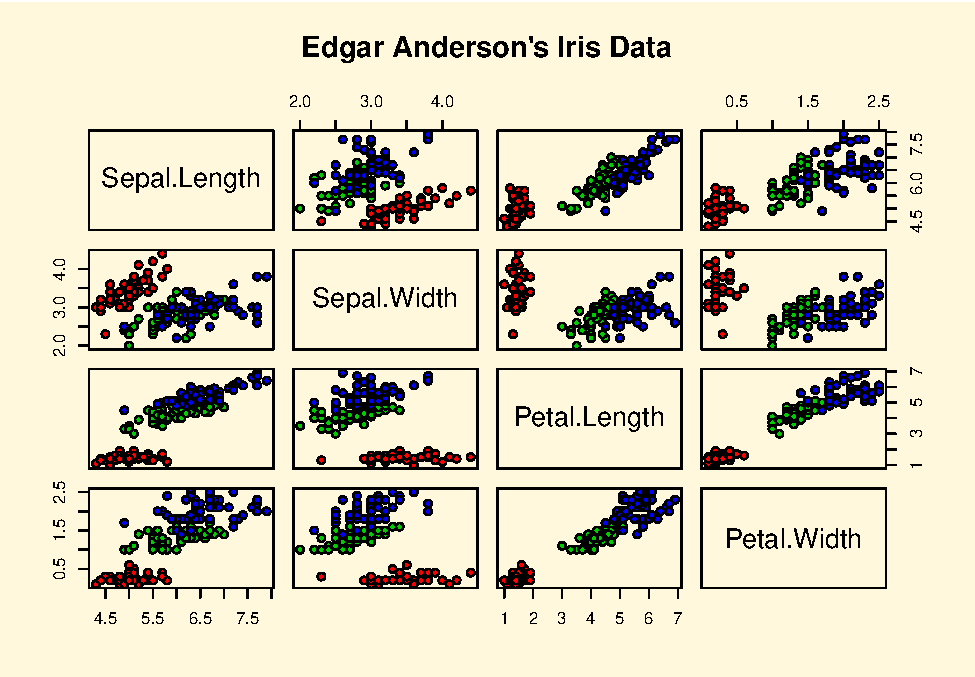
\includegraphics{bookdown-demo_files/figure-latex/unnamed-chunk-5-9.pdf}

\begin{verbatim}
## 
## > ## Contour plotting
## > ## This produces a topographic map of one of Auckland's many volcanic "peaks".
## > 
## > x <- 10*1:nrow(volcano)
## 
## > y <- 10*1:ncol(volcano)
## 
## > lev <- pretty(range(volcano), 10)
## 
## > par(bg = "lightcyan")
## 
## > pin <- par("pin")
## 
## > xdelta <- diff(range(x))
## 
## > ydelta <- diff(range(y))
## 
## > xscale <- pin[1]/xdelta
## 
## > yscale <- pin[2]/ydelta
## 
## > scale <- min(xscale, yscale)
## 
## > xadd <- 0.5*(pin[1]/scale - xdelta)
## 
## > yadd <- 0.5*(pin[2]/scale - ydelta)
## 
## > plot(numeric(0), numeric(0),
## +      xlim = range(x)+c(-1,1)*xadd, ylim = range(y)+c(-1,1)*yadd,
## +      type = "n", ann = FALSE)
\end{verbatim}

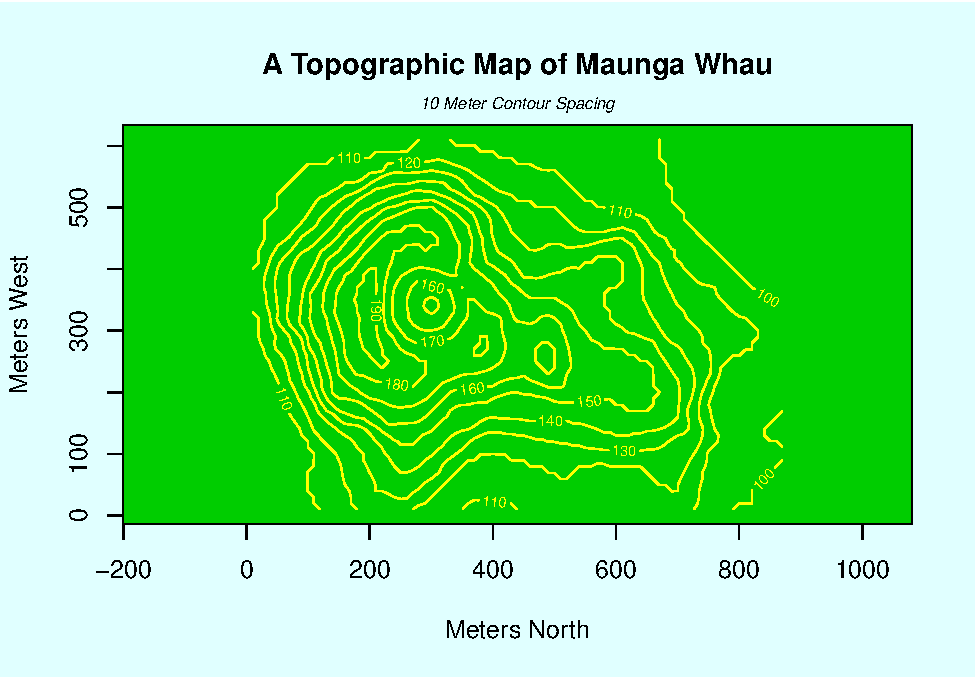
\includegraphics{bookdown-demo_files/figure-latex/unnamed-chunk-5-10.pdf}

\begin{verbatim}
## 
## > usr <- par("usr")
## 
## > rect(usr[1], usr[3], usr[2], usr[4], col="green3")
## 
## > contour(x, y, volcano, levels = lev, col="yellow", lty="solid", add=TRUE)
## 
## > box()
## 
## > title("A Topographic Map of Maunga Whau", font= 4)
## 
## > title(xlab = "Meters North", ylab = "Meters West", font= 3)
## 
## > mtext("10 Meter Contour Spacing", side=3, line=0.35, outer=FALSE,
## +       at = mean(par("usr")[1:2]), cex=0.7, font=3)
## 
## > ## Conditioning plots
## > 
## > par(bg="cornsilk")
## 
## > coplot(lat ~ long | depth, data = quakes, pch = 21, bg = "green3")
\end{verbatim}

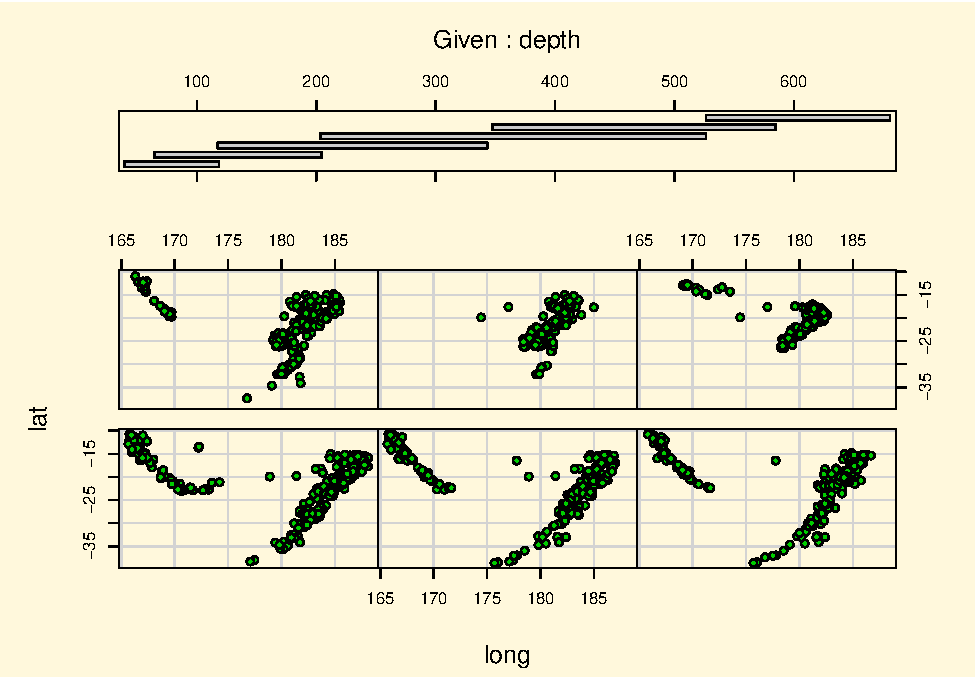
\includegraphics{bookdown-demo_files/figure-latex/unnamed-chunk-5-11.pdf}

\begin{verbatim}
## 
## > par(opar)
\end{verbatim}

\textbf{Ejercicios}

\begin{enumerate}
\def\labelenumi{\arabic{enumi}.}
\tightlist
\item
  Instala las siguientes librerías que te serviran durante todo el curso

  \begin{itemize}
  \tightlist
  \item
    markdown
  \item
    ggplot2
  \end{itemize}
\end{enumerate}

\textbf{INFORMACIÓN ADICIONAL}

Existen repositorios adicionales a \href{https://cran.r-project.org/}{CRAN}, uno de ellos es \href{https://https://bioconductor.org/}{Bioconductor}, en él puedes buscar e instalar paquetes como \texttt{ggtree}.

\textbf{Ejercicio}
1. Explora la página de Bioconductor, apóyate de su buscador e instala el paquete \texttt{ggtree}.

\hypertarget{ayuda-en-r}{%
\section{Ayuda en R}\label{ayuda-en-r}}

En la mayoría de las ocasiones desconocemos el alcance de alguna paquetería, los criterios de alguna función o en general, sabemos lo que queremos hacer pero no tenemos ni idea de qué paqueteria usar.

Los comandos \texttt{help()} y \texttt{?} son equivalentes, ambos van a permitir encontrar información sobre paqueterias, comandos o funciones generales de R. Se debe teclear \texttt{help(nombre\_comando)} o \texttt{?nombre\_comando}

Por ejemplo, para buscar información detallada del comando solve:

\begin{Shaded}
\begin{Highlighting}[]
\FunctionTok{help}\NormalTok{(solve)}
\end{Highlighting}
\end{Shaded}

\begin{Shaded}
\begin{Highlighting}[]
\NormalTok{?solve}
\end{Highlighting}
\end{Shaded}

Para buscar ayuda de funciones o palabra reservadas se utilizan comillas:

\begin{Shaded}
\begin{Highlighting}[]
\FunctionTok{help}\NormalTok{(}\StringTok{"for"}\NormalTok{)}
\end{Highlighting}
\end{Shaded}

También existen opciones como \texttt{help.start()} y \texttt{help.search()} para obtener una versión extendida de la ayuda general desplegada en un navegador. Para ello se requiere tener la ayuda en HTML instalada y conexión a la red.

\texttt{help.search()} es una función que escanea documentación para paquetes previamente instalados.

Ejemplo:

\begin{Shaded}
\begin{Highlighting}[]
\FunctionTok{help.search}\NormalTok{(}\StringTok{"clustering"}\NormalTok{)}
\end{Highlighting}
\end{Shaded}

\texttt{help.start()} es una función que despliega información basada en documentos en línea de la versión actual de R, además de brindar links a manuales y la lista de las paqueterías instaladas, entre otras cosas.

Ejemplo:

\begin{Shaded}
\begin{Highlighting}[]
\FunctionTok{help.start}\NormalTok{()}
\end{Highlighting}
\end{Shaded}

Cuando queremos ver ejemplos del uso de los comandos usamos la función \texttt{example()}

Ejemplo:

\begin{Shaded}
\begin{Highlighting}[]
\FunctionTok{example}\NormalTok{(}\StringTok{"hclust"}\NormalTok{)}
\end{Highlighting}
\end{Shaded}

\begin{verbatim}
## 
## hclust> require(graphics)
## 
## hclust> ### Example 1: Violent crime rates by US state
## hclust> 
## hclust> hc <- hclust(dist(USArrests), "ave")
## 
## hclust> plot(hc)
\end{verbatim}

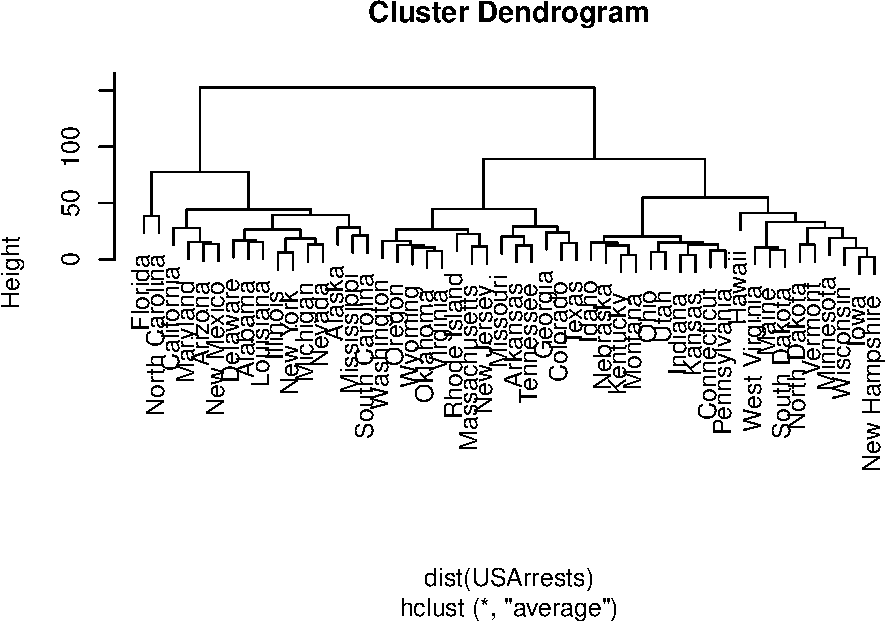
\includegraphics{bookdown-demo_files/figure-latex/unnamed-chunk-11-1.pdf}

\begin{verbatim}
## 
## hclust> plot(hc, hang = -1)
\end{verbatim}

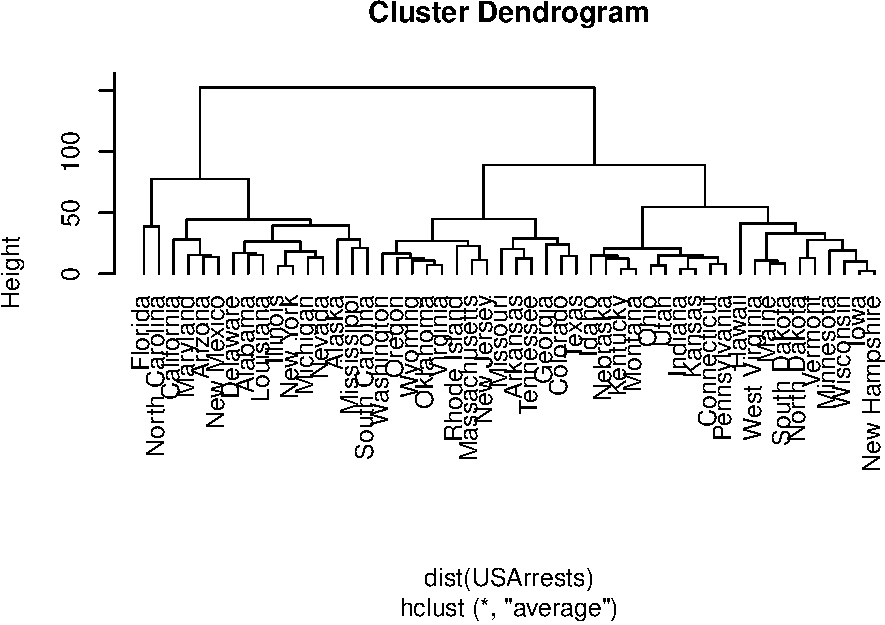
\includegraphics{bookdown-demo_files/figure-latex/unnamed-chunk-11-2.pdf}

\begin{verbatim}
## 
## hclust> ## Do the same with centroid clustering and *squared* Euclidean distance,
## hclust> ## cut the tree into ten clusters and reconstruct the upper part of the
## hclust> ## tree from the cluster centers.
## hclust> hc <- hclust(dist(USArrests)^2, "cen")
## 
## hclust> memb <- cutree(hc, k = 10)
## 
## hclust> cent <- NULL
## 
## hclust> for(k in 1:10){
## hclust+   cent <- rbind(cent, colMeans(USArrests[memb == k, , drop = FALSE]))
## hclust+ }
## 
## hclust> hc1 <- hclust(dist(cent)^2, method = "cen", members = table(memb))
## 
## hclust> opar <- par(mfrow = c(1, 2))
## 
## hclust> plot(hc,  labels = FALSE, hang = -1, main = "Original Tree")
\end{verbatim}

\begin{verbatim}
## 
## hclust> plot(hc1, labels = FALSE, hang = -1, main = "Re-start from 10 clusters")
\end{verbatim}

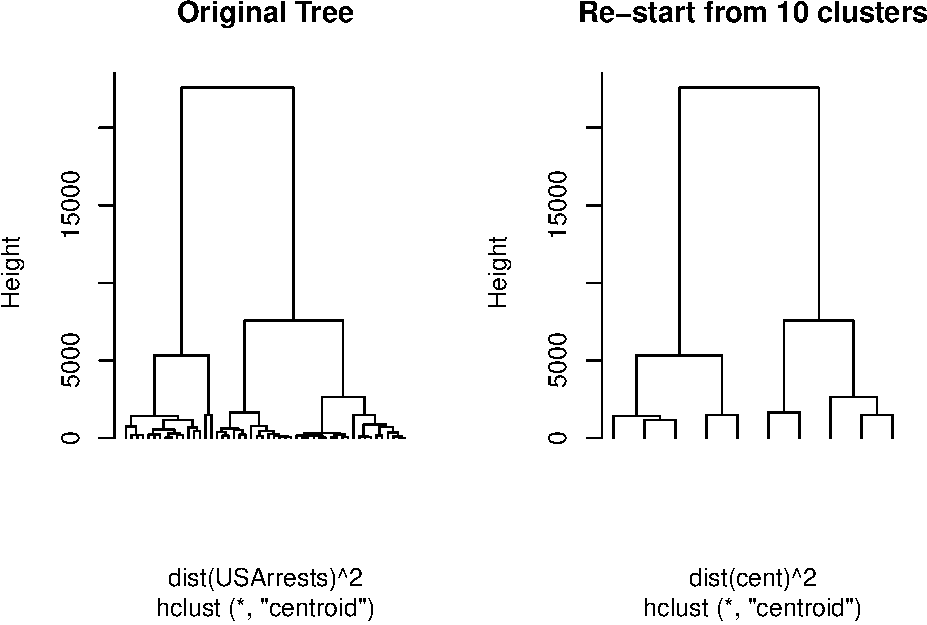
\includegraphics{bookdown-demo_files/figure-latex/unnamed-chunk-11-3.pdf}

\begin{verbatim}
## 
## hclust> par(opar)
## 
## hclust> ### Example 2: Straight-line distances among 10 US cities
## hclust> ##  Compare the results of algorithms "ward.D" and "ward.D2"
## hclust> 
## hclust> mds2 <- -cmdscale(UScitiesD)
## 
## hclust> plot(mds2, type="n", axes=FALSE, ann=FALSE)
\end{verbatim}

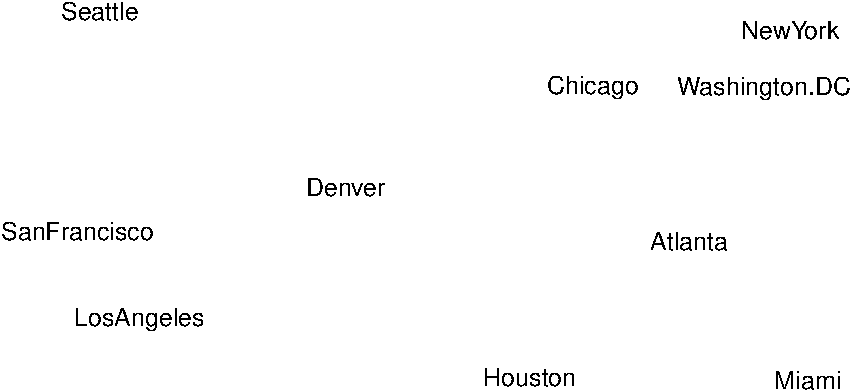
\includegraphics{bookdown-demo_files/figure-latex/unnamed-chunk-11-4.pdf}

\begin{verbatim}
## 
## hclust> text(mds2, labels=rownames(mds2), xpd = NA)
## 
## hclust> hcity.D  <- hclust(UScitiesD, "ward.D") # "wrong"
## 
## hclust> hcity.D2 <- hclust(UScitiesD, "ward.D2")
## 
## hclust> opar <- par(mfrow = c(1, 2))
## 
## hclust> plot(hcity.D,  hang=-1)
\end{verbatim}

\begin{verbatim}
## 
## hclust> plot(hcity.D2, hang=-1)
\end{verbatim}

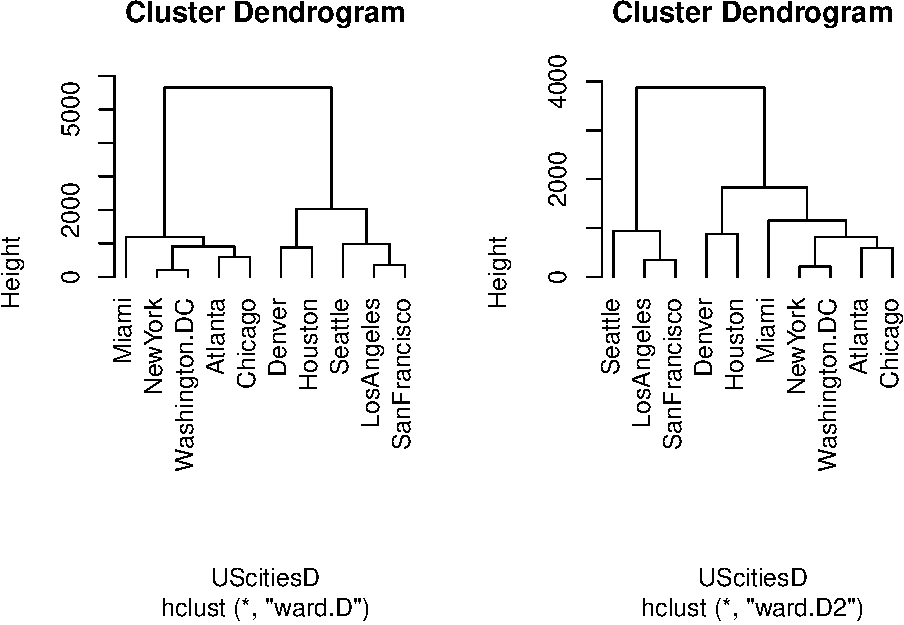
\includegraphics{bookdown-demo_files/figure-latex/unnamed-chunk-11-5.pdf}

\begin{verbatim}
## 
## hclust> par(opar)
\end{verbatim}

Todo lo anterior requiere que conozcamos el nombre correcto del comando, pero ¿qué pasa si no lo sabemos?, ¿lloramos? no.
Podemos utilizar el comando \texttt{apropos()} para encontrar todo lo relacionado con algún término.

Ejemplo:

\begin{Shaded}
\begin{Highlighting}[]
\FunctionTok{apropos}\NormalTok{(}\StringTok{"solve"}\NormalTok{)}
\end{Highlighting}
\end{Shaded}

\begin{verbatim}
##  [1] ".rs.markdown.resolveCompletionRoot" ".rs.resolveAliasedPath"            
##  [3] ".rs.resolveAliasedSymbol"           ".rs.resolveContextSourceRefs"      
##  [5] ".rs.resolveEnvironment"             ".rs.resolveFormals"                
##  [7] ".rs.resolveFormalsImpl"             ".rs.resolveFormalsImplS3Dispatch"  
##  [9] ".rs.resolveObjectFromFunctionCall"  ".rs.resolveObjectSource"           
## [11] ".rs.reticulate.resolveModule"       ".rs.rnb.resolveActiveChunkId"      
## [13] "backsolve"                          "forwardsolve"                      
## [15] "qr.solve"                           "solve"                             
## [17] "solve.default"                      "solve.qr"
\end{verbatim}

Ahora, ¿qué pasa cuando tengo la idea de lo que quiero hacer pero no se qué paqueteria usar, ni cuál comando? puedo usar \texttt{??} seguido de una palabra clave. Esto nos arrojará sugerencias sobre lo que deseamos hacer.

Ejemplo:

\begin{Shaded}
\begin{Highlighting}[]
\NormalTok{??DNA}
\end{Highlighting}
\end{Shaded}

\textbf{NOTA} Se recomienda el uso del autocompletado, de esta manera reducirás errores de dedo.

\hypertarget{expresiones-y-asignaciones}{%
\section{Expresiones y asignaciones}\label{expresiones-y-asignaciones}}

Las \textbf{expresiones} y \textbf{asignaciones} son los dos tipos de resultados que arroja R.

Las \textbf{expresiones} sólo se muestran en la salida estándar y NO se guardan en alguna variable, es decir, cada que se corra la línea se obtendran valores distintos.

Ejemplo:

\begin{Shaded}
\begin{Highlighting}[]
\FunctionTok{rnorm}\NormalTok{(}\DecValTok{10}\NormalTok{)}
\end{Highlighting}
\end{Shaded}

\begin{verbatim}
##  [1] -0.3662005  0.5282137  1.0297297  1.2026469 -0.2471466  0.4881020
##  [7]  0.2574261  1.8267633 -0.6307991 -0.7868046
\end{verbatim}

\begin{Shaded}
\begin{Highlighting}[]
\FunctionTok{rnorm}\NormalTok{(}\DecValTok{10}\NormalTok{)}
\end{Highlighting}
\end{Shaded}

\begin{verbatim}
##  [1]  0.43151411  0.61228772 -0.25996672  0.86093387 -1.81208295 -0.56694057
##  [7] -0.53656818  0.01307127  0.78333265  0.36506122
\end{verbatim}

Las \textbf{asignaciones}, como su nombre lo indica, se guardan los valores al ser asignados a una variable. Esto se puede lograr mediante el uso de \texttt{\textless{}-}

Ejemplo:

\begin{Shaded}
\begin{Highlighting}[]
\NormalTok{x }\OtherTok{\textless{}{-}} \FunctionTok{rnorm}\NormalTok{(}\DecValTok{10}\NormalTok{)}
\end{Highlighting}
\end{Shaded}

\begin{Shaded}
\begin{Highlighting}[]
\NormalTok{x}
\end{Highlighting}
\end{Shaded}

\begin{verbatim}
##  [1]  1.0563450 -1.0324512 -2.4032323 -1.8183751  0.9790058  0.8870176
##  [7]  0.2704107  0.6102592  0.3311577 -1.2497648
\end{verbatim}

\textbf{NOTA} El símbolo \texttt{\textless{}-} es equivalente en función a \texttt{=} pero no es tan cool.

\begin{figure}
\centering

\includegraphics{equals-sign-assignment-operator-imgflip-com-going-through-data-structures-and-47188178.png}
\caption{Operador de asignación. Así que evita el uso del igual}
\end{figure}

Otro punto a considerar respecto a las \textbf{asiganciones} es que R es capaz de distinguir entre mayúsculas y minúsculas, por lo que la misma letra puede contener valores distintos.

Ejemplo:

\begin{Shaded}
\begin{Highlighting}[]
\NormalTok{a }\OtherTok{\textless{}{-}} \DecValTok{3}
\NormalTok{A }\OtherTok{\textless{}{-}} \DecValTok{6}
\end{Highlighting}
\end{Shaded}

\begin{Shaded}
\begin{Highlighting}[]
\NormalTok{a}
\end{Highlighting}
\end{Shaded}

\begin{verbatim}
## [1] 3
\end{verbatim}

\begin{Shaded}
\begin{Highlighting}[]
\NormalTok{A}
\end{Highlighting}
\end{Shaded}

\begin{verbatim}
## [1] 6
\end{verbatim}

Una opción es definirlas en más de una línea, ejemplo:

\begin{Shaded}
\begin{Highlighting}[]
\NormalTok{a }\OtherTok{\textless{}{-}}
\NormalTok{  pi }\SpecialCharTok{+} \DecValTok{12}
\end{Highlighting}
\end{Shaded}

\textbf{NOTA} Ten mucha precaución con el nombre que asignas a un valor, ya que podrías sobreescribirlo y se le quedará asignado el último valor.

Ejemplo:

\begin{Shaded}
\begin{Highlighting}[]
\NormalTok{b }\OtherTok{\textless{}{-}} \DecValTok{3}
\NormalTok{b}
\end{Highlighting}
\end{Shaded}

\begin{verbatim}
## [1] 3
\end{verbatim}

\begin{Shaded}
\begin{Highlighting}[]
\NormalTok{b }\OtherTok{\textless{}{-}} \DecValTok{8} 
\NormalTok{b}
\end{Highlighting}
\end{Shaded}

\begin{verbatim}
## [1] 8
\end{verbatim}

La separación de comandos puede darse de dos formas:

Empleando \texttt{;}, ejemplo:

\begin{Shaded}
\begin{Highlighting}[]
\NormalTok{a }\OtherTok{\textless{}{-}} \DecValTok{3}\NormalTok{; b }\OtherTok{\textless{}{-}}\DecValTok{5}
\end{Highlighting}
\end{Shaded}

o usando un salto de línea, esta es una mejor opción, ejemplo:

\begin{Shaded}
\begin{Highlighting}[]
\NormalTok{a }\OtherTok{\textless{}{-}} \DecValTok{3}
\NormalTok{b }\OtherTok{\textless{}{-}}\DecValTok{5}
\end{Highlighting}
\end{Shaded}

\hypertarget{movimiento-entre-directorios}{%
\section{Movimiento entre directorios}\label{movimiento-entre-directorios}}

Otra de las ventajas que ofrece R es que permite ubicar algún archivo o saber la dirección del directorio en la que nos encontramos actualmente, todo ello sin necesidad de salir de la interfaz.

Para saber en qué directorio estamos, se teclea:

\begin{Shaded}
\begin{Highlighting}[]
\FunctionTok{getwd}\NormalTok{()}
\end{Highlighting}
\end{Shaded}

\begin{verbatim}
## [1] "/Users/robertoalvarez/Dropbox/Manual_Bravo_Marifer_Bioinfo_2024"
\end{verbatim}

Para cambiar de directorio utilizamos \texttt{setwd("direccion\_a\_la\_que\_quieres\_ir")}

\begin{Shaded}
\begin{Highlighting}[]
\FunctionTok{setwd}\NormalTok{(}\StringTok{"\textasciitilde{}"}\NormalTok{)}
\end{Highlighting}
\end{Shaded}

\#\#Bash en R
También se pueden usar los comandos de la terminal de bash dentro de R, utilizando la función \texttt{system()}

Para listar archivos de una carpeta usamos \texttt{ls}

\begin{Shaded}
\begin{Highlighting}[]
\FunctionTok{system}\NormalTok{(}\StringTok{"ls {-}la"}\NormalTok{)}
\end{Highlighting}
\end{Shaded}

Para saber en qué directorio estamos usamos la función análoga a \texttt{getwd()}, que es \texttt{pwd}

\begin{Shaded}
\begin{Highlighting}[]
\FunctionTok{system}\NormalTok{(}\StringTok{"pwd"}\NormalTok{)}
\end{Highlighting}
\end{Shaded}

\textbf{Importante: Como regla general todos los nombres van entre comillas: nombre de carpetas, archivos, de columnas, de renglones,etc.}

\hypertarget{operaciones-aritmuxe9ticas}{%
\section{Operaciones aritméticas}\label{operaciones-aritmuxe9ticas}}

R también puede ser usado como calculadora.
Se puede sumar, restar, multiplicar,dividir, ``exponenciar'' y calcular la raíz cuadrada.

\textbf{SUMA} con el operador \texttt{+}

\begin{Shaded}
\begin{Highlighting}[]
\NormalTok{a }\SpecialCharTok{+}\NormalTok{ b}
\end{Highlighting}
\end{Shaded}

\begin{verbatim}
## [1] 8
\end{verbatim}

\textbf{RESTA} con el operador \texttt{-}

\begin{Shaded}
\begin{Highlighting}[]
\NormalTok{a }\SpecialCharTok{{-}}\NormalTok{ b}
\end{Highlighting}
\end{Shaded}

\begin{verbatim}
## [1] -2
\end{verbatim}

\textbf{MULTIPLICACIÓN} con el operador \texttt{*}

\begin{Shaded}
\begin{Highlighting}[]
\NormalTok{a }\SpecialCharTok{*}\NormalTok{ b}
\end{Highlighting}
\end{Shaded}

\begin{verbatim}
## [1] 15
\end{verbatim}

\textbf{DIVISIÓN} con el operador \texttt{/}

\begin{Shaded}
\begin{Highlighting}[]
\NormalTok{a }\SpecialCharTok{/}\NormalTok{ b}
\end{Highlighting}
\end{Shaded}

\begin{verbatim}
## [1] 0.6
\end{verbatim}

\textbf{EXPONENTE} con los operadoradores \texttt{**} o \texttt{\^{}}

\begin{Shaded}
\begin{Highlighting}[]
\NormalTok{a }\SpecialCharTok{**}\NormalTok{ b}
\end{Highlighting}
\end{Shaded}

\begin{verbatim}
## [1] 243
\end{verbatim}

\begin{Shaded}
\begin{Highlighting}[]
\NormalTok{a }\SpecialCharTok{\^{}}\NormalTok{ b}
\end{Highlighting}
\end{Shaded}

\begin{verbatim}
## [1] 243
\end{verbatim}

\textbf{RAÍZ CUADRADA} con la función \texttt{sqrt()}

\begin{Shaded}
\begin{Highlighting}[]
\FunctionTok{sqrt}\NormalTok{(a)}
\end{Highlighting}
\end{Shaded}

\begin{verbatim}
## [1] 1.732051
\end{verbatim}

\textbf{LOGARITMO} con la función \texttt{log()}

\begin{Shaded}
\begin{Highlighting}[]
\FunctionTok{log}\NormalTok{(a)}
\end{Highlighting}
\end{Shaded}

\begin{verbatim}
## [1] 1.098612
\end{verbatim}

\hypertarget{prioridad-en-las-operaciones}{%
\subsection{Prioridad en las operaciones}\label{prioridad-en-las-operaciones}}

Las operaciones se efectuan en el siguiente orden:

\begin{enumerate}
\def\labelenumi{\arabic{enumi}.}
\tightlist
\item
  izquierda a derecha
\item
  \texttt{sqrt()} y \texttt{**} \texttt{\^{}}
\item
  \texttt{*} y \texttt{/}
\item
  \texttt{+} y \texttt{-}
\item
  \texttt{\textless{}-}
\end{enumerate}

\emph{IMPORTANTE} Este orden se altera si se presenta un paréntesis. En ese caso la operación dentro del paréntesis es la que se realiza primero.

Ejemplos:

\texttt{4\ +\ 2\ *\ 3\ =\ 4\ +\ 6\ =\ 10}

\texttt{4\ -\ 15/3\ +\ 3\^{}2\ +\ sqrt(9)\ =\ 4\ -\ 15/3\ +\ 9\ +\ 3\ =\ 4\ -\ 5\ +\ 12\ =\ 13}

\texttt{4\ -\ (3+7)\^{}2\ +\ (2+3)/5\ =\ 4\ -\ (10)\^{}2\ +\ 5/5\ =\ 4\ -\ 100\ +\ 1\ =\ -95}

\textbf{Ejercicios}

Resuelve en un pedazo de papel primero para saber cuál sería el resultado de las siguientes operaciones aritméticas. Después comprueba tu resultado tecleandolas en R.

\begin{enumerate}
\def\labelenumi{\arabic{enumi}.}
\tightlist
\item
  1 + 2*3 + 3 + 15/3
\item
  4 - 15/3 + 3\^{}2 + 3*sqrt(81)
\item
  40 - (4+3)\^{}2 + (10-5)/3
\item
  32\^{}5 - (3-5)*2 + 32/sqrt(64)
\item
  1/(3\^{}-3) + (8-10\^{}2) - (25/sqrt(25))\^{}2
\end{enumerate}

\hypertarget{tipos-de-valores-en-r}{%
\section{Tipos de valores en R}\label{tipos-de-valores-en-r}}

\hypertarget{valores-booleanos}{%
\subsection{Valores booleanos}\label{valores-booleanos}}

También conocidos como \emph{Datos lógicos}.
Este tipo de datos \textbf{sólo} contienen información \texttt{TRUE} o \texttt{FALSE}, lo cual sirve para evaluar si los elementos de un vector cumplen con los criterios deseados. Para ello se utilizan los operadores de comparación:

\begin{itemize}
\tightlist
\item
  igual \texttt{==}
\item
  no es igual a \texttt{!=}
\item
  menor que \texttt{\textless{}}
\item
  mayor que \texttt{\textgreater{}}
\item
  menor o igual que \texttt{\textless{}=}
\item
  mayor o igual que \texttt{\textgreater{}=}
\end{itemize}

Ejemplo:

\begin{Shaded}
\begin{Highlighting}[]
\DecValTok{1} \SpecialCharTok{\textless{}} \DecValTok{5}
\end{Highlighting}
\end{Shaded}

\begin{verbatim}
## [1] TRUE
\end{verbatim}

\begin{Shaded}
\begin{Highlighting}[]
\DecValTok{10} \SpecialCharTok{==} \DecValTok{0}    
\end{Highlighting}
\end{Shaded}

\begin{verbatim}
## [1] FALSE
\end{verbatim}

\begin{Shaded}
\begin{Highlighting}[]
\DecValTok{10} \SpecialCharTok{!=} \DecValTok{0}   
\end{Highlighting}
\end{Shaded}

\begin{verbatim}
## [1] TRUE
\end{verbatim}

\begin{Shaded}
\begin{Highlighting}[]
\DecValTok{10} \SpecialCharTok{\textless{}=} \DecValTok{0}   
\end{Highlighting}
\end{Shaded}

\begin{verbatim}
## [1] FALSE
\end{verbatim}

\textbf{NOTA} Dentro de R los valores lógicos \texttt{TRUE} y \texttt{FALSE} tienen un valor numérico. \texttt{TRUE}equivale a 1 y \texttt{FALSE} es equivalente a 0. Esto permite cuantificar el número de elementos que cumplen con los criterios, ¿cómo? mediante la suma de los \texttt{TRUE}s.

\textbf{Ejercicios}
Demuestra si:
1. El logaritmo base 10 de 20 es menor que la raíz cuadrada de 4. Desarrollalo en una sola línea.
2. 1/3\^{}-1 es igual a 3/1\^{}-1
3. (-2)\^{}2 no es igual a (2)\^{}2

\hypertarget{caracter}{%
\subsection{Caracter}\label{caracter}}

Son \emph{strings} de texto y se caracterizan porque cada uno de los elementos va entre comillas. Los elementos pueden ser desde sólo un caracter hasta oraciones.
Podría parecer que la variable a la cual lo asignamos contiene números, pero las comillas indican que serán tratados como texto. Podemos subsetearlos por su índice o buscando literalmente el texto.

Ejemplo:

\begin{Shaded}
\begin{Highlighting}[]
\NormalTok{x}\OtherTok{\textless{}{-}} \StringTok{"La candente mañana de febrero en que Beatriz Viterbo murió, después de una imperiosa agonía que no se rebajó un solo instante ni al sentimentalismo ni al miedo"}
\end{Highlighting}
\end{Shaded}

\hypertarget{enteros-y-nuxfameros-numeric}{%
\subsection{Enteros y números (numeric)}\label{enteros-y-nuxfameros-numeric}}

Existen dos formas diferentes en que las computadoras pueden guardar los números y hacer operaciones matemáticas con ellos: \texttt{numeric} e \texttt{integer}.
Por lo común no importa esta diferencia, pero puede ser relevante para algunas funciones de Bioconductor. En R se representan los números como \texttt{numeric} y el tamaño máximo que maneja para un \texttt{integer} es ligeramente más chico que el tamaño del genoma humano.

¿Cómo revisar si un objeto es numeric o entero? Con la función \texttt{class()}

\begin{Shaded}
\begin{Highlighting}[]
\NormalTok{x }\OtherTok{\textless{}{-}} \DecValTok{1}
\FunctionTok{class}\NormalTok{(x)}
\end{Highlighting}
\end{Shaded}

\begin{verbatim}
## [1] "numeric"
\end{verbatim}

\begin{Shaded}
\begin{Highlighting}[]
\NormalTok{x }\OtherTok{\textless{}{-}} \DecValTok{1}\SpecialCharTok{:}\DecValTok{3}
\FunctionTok{class}\NormalTok{(x)}
\end{Highlighting}
\end{Shaded}

\begin{verbatim}
## [1] "integer"
\end{verbatim}

\hypertarget{estructura}{%
\chapter{Vectores}\label{estructura}}

R permite manejar datos dentro de estructuras para poder trabajarlos, estas estructuras pueden ser:
- Vector: Es de una sola dimensión y solo permite almacenar datos del mismo tipo.
- Matriz: Es un arreglo en dos dimensiones y permite ingresar datos del mismo tipo.
- Data Frame: Similar a la matriz por ser también de dos dimensiones, solo que este arreglo permite distintas clases de datos.
- Lista: Es de una sola dimensión como el vector, la diferencia que es que una lista permite incorporar diferentes tipos de datos.

\hypertarget{contenido}{%
\section{Contenido}\label{contenido}}

Para conocer el contenido de una variable, sólo es necesario poner la variable y presionar \emph{enter} (sesión interactiva). En el caso de estar en un \emph{script} es necesario usar la función \texttt{print()}

Ejemplo:

\begin{Shaded}
\begin{Highlighting}[]
\NormalTok{x}\OtherTok{\textless{}{-}}\DecValTok{3}
\FunctionTok{print}\NormalTok{(x)}
\end{Highlighting}
\end{Shaded}

\begin{verbatim}
## [1] 3
\end{verbatim}

\hypertarget{vectors}{%
\section{Vectores en R}\label{vectors}}

Un \emph{vector} es una colección de datos del mismo tipo, siempre del \textbf{mismo tipo}, no es posible mezclarlos. Los elementos contenidos dentro de un vector son conocidos como \emph{componentes} y pueden ser del tipo lógico, caracteres, numéricos o integer.

\hypertarget{definiciuxf3n}{%
\section{Definición}\label{definiciuxf3n}}

Para definir un vector se utiliza la función \texttt{c()}, que significa \emph{combine}.
Existen dos formas de definir un vector: \textbf{Extensiva} y \textbf{Secuencia}.

\hypertarget{definiciuxf3n-extensiva}{%
\subsection{Definición extensiva}\label{definiciuxf3n-extensiva}}

La \textbf{forma extensiva} para definir un vector considera que los elementos situados dentro del paréntesis tienen que estar separados por comas.

Ejemplo:

\begin{Shaded}
\begin{Highlighting}[]
\NormalTok{vector\_numerico }\OtherTok{\textless{}{-}} \FunctionTok{c}\NormalTok{(}\DecValTok{1}\NormalTok{, }\DecValTok{3}\NormalTok{, }\DecValTok{5}\NormalTok{, }\DecValTok{7}\NormalTok{)      }\CommentTok{\# vector numérico}
\NormalTok{vector\_texto }\OtherTok{\textless{}{-}} \FunctionTok{c}\NormalTok{(}\StringTok{"a"}\NormalTok{, }\StringTok{"b"}\NormalTok{, }\StringTok{"c"}\NormalTok{, }\StringTok{"d"}\NormalTok{) }\CommentTok{\# vector de texto}
\NormalTok{vector\_logico }\OtherTok{\textless{}{-}} \FunctionTok{c}\NormalTok{(}\ConstantTok{TRUE}\NormalTok{, }\ConstantTok{FALSE}\NormalTok{, }\ConstantTok{TRUE}\NormalTok{) }\CommentTok{\# vector lógico / booleano}
\end{Highlighting}
\end{Shaded}

\hypertarget{definiciuxf3n-en-secuencia}{%
\subsection{Definición en secuencia}\label{definiciuxf3n-en-secuencia}}

\hypertarget{uso-de-c}{%
\subsubsection{Uso de c()}\label{uso-de-c}}

En algunas ocasiones definir de manera extensiva puede resultar muy poco eficiente, sobre todo para vectores que contengan una gran cantidad de elementos en secuencia, para ello se definen en \textbf{forma de secuencia} empleando el operador \texttt{:}.

Ejemplo:
Un vector que tenga los primeros 100 números enteros

\begin{Shaded}
\begin{Highlighting}[]
\NormalTok{x }\OtherTok{\textless{}{-}} \FunctionTok{c}\NormalTok{(}\DecValTok{1}\SpecialCharTok{:}\DecValTok{100}\NormalTok{)}

\NormalTok{x}
\end{Highlighting}
\end{Shaded}

\begin{verbatim}
##   [1]   1   2   3   4   5   6   7   8   9  10  11  12  13  14  15  16  17  18
##  [19]  19  20  21  22  23  24  25  26  27  28  29  30  31  32  33  34  35  36
##  [37]  37  38  39  40  41  42  43  44  45  46  47  48  49  50  51  52  53  54
##  [55]  55  56  57  58  59  60  61  62  63  64  65  66  67  68  69  70  71  72
##  [73]  73  74  75  76  77  78  79  80  81  82  83  84  85  86  87  88  89  90
##  [91]  91  92  93  94  95  96  97  98  99 100
\end{verbatim}

\hypertarget{uso-de-seq}{%
\subsubsection{Uso de seq()}\label{uso-de-seq}}

Otra alternativa es la función \texttt{seq()} que significa \emph{sequence} y es una generalización del operador \texttt{:}.

Ejemplo:

\begin{Shaded}
\begin{Highlighting}[]
\NormalTok{x }\OtherTok{\textless{}{-}} \FunctionTok{seq}\NormalTok{(}\DecValTok{1}\NormalTok{,}\DecValTok{100}\NormalTok{)}

\NormalTok{x}
\end{Highlighting}
\end{Shaded}

\begin{verbatim}
##   [1]   1   2   3   4   5   6   7   8   9  10  11  12  13  14  15  16  17  18
##  [19]  19  20  21  22  23  24  25  26  27  28  29  30  31  32  33  34  35  36
##  [37]  37  38  39  40  41  42  43  44  45  46  47  48  49  50  51  52  53  54
##  [55]  55  56  57  58  59  60  61  62  63  64  65  66  67  68  69  70  71  72
##  [73]  73  74  75  76  77  78  79  80  81  82  83  84  85  86  87  88  89  90
##  [91]  91  92  93  94  95  96  97  98  99 100
\end{verbatim}

Esta función permite generar secuencias numéricas de distintas clase y por diferentes rangos.

Ejemplo:
Una secuencia que vaya desde -12 hasta 30 en un rango de 3, es decir, -12, -9, -6, \ldots, 27, 30:

\begin{Shaded}
\begin{Highlighting}[]
\NormalTok{x }\OtherTok{\textless{}{-}} \FunctionTok{seq}\NormalTok{(}\AttributeTok{from=}\SpecialCharTok{{-}}\DecValTok{12}\NormalTok{,}\AttributeTok{to=}\DecValTok{30}\NormalTok{,}\AttributeTok{by=}\DecValTok{3}\NormalTok{)}

\NormalTok{x}
\end{Highlighting}
\end{Shaded}

\begin{verbatim}
##  [1] -12  -9  -6  -3   0   3   6   9  12  15  18  21  24  27  30
\end{verbatim}

\textbf{NOTA} Se puede omitir \emph{from}, \emph{to} y \emph{by} mientras se sigan colocando los valores en el mismo orden.

Ejemplo:

\begin{Shaded}
\begin{Highlighting}[]
\NormalTok{y }\OtherTok{\textless{}{-}} \FunctionTok{seq}\NormalTok{(}\DecValTok{0}\NormalTok{,}\DecValTok{1}\NormalTok{,}\FloatTok{0.1}\NormalTok{)}

\NormalTok{y}
\end{Highlighting}
\end{Shaded}

\begin{verbatim}
##  [1] 0.0 0.1 0.2 0.3 0.4 0.5 0.6 0.7 0.8 0.9 1.0
\end{verbatim}

\textbf{NOTA} Si queremos cambiar el orden, debemos necesariamente ponerlos.
Ejemplo:

\begin{Shaded}
\begin{Highlighting}[]
\NormalTok{z }\OtherTok{\textless{}{-}} \FunctionTok{seq}\NormalTok{(}\AttributeTok{by=}\FloatTok{0.1}\NormalTok{, }\AttributeTok{to =}\DecValTok{1}\NormalTok{, }\AttributeTok{from=}\FloatTok{0.5}\NormalTok{)}

\NormalTok{z}
\end{Highlighting}
\end{Shaded}

\begin{verbatim}
## [1] 0.5 0.6 0.7 0.8 0.9 1.0
\end{verbatim}

\hypertarget{longitud-de-un-vector}{%
\section{Longitud de un vector}\label{longitud-de-un-vector}}

La \emph{longitud} de un vector se refiere al número de elementos que contiene. Para conocer ese dato se emplea la función \texttt{length()}

Ejemplo:

\begin{Shaded}
\begin{Highlighting}[]
\NormalTok{s }\OtherTok{\textless{}{-}}\NormalTok{ (}\DecValTok{1}\SpecialCharTok{:}\DecValTok{5}\NormalTok{)}

\FunctionTok{length}\NormalTok{(s)}
\end{Highlighting}
\end{Shaded}

\begin{verbatim}
## [1] 5
\end{verbatim}

\hypertarget{elementos-de-un-vector}{%
\section{Elementos de un vector}\label{elementos-de-un-vector}}

Para acceder a elementos de un objeto con \emph{indices} (componentes que tienen una posición asignada), debemos usar \emph{corchetes} \texttt{{[}{]}}. Los corchetes pueden contener posiciones consecutivas o no consecutivas.

\hypertarget{elementos-consecutivos}{%
\subsection{Elementos consecutivos}\label{elementos-consecutivos}}

Se definen el rango de las posiciones a seleccionar, para ello se emplea el operador \texttt{:}

Ejemplo:

\begin{Shaded}
\begin{Highlighting}[]
\CommentTok{\#Se define el vector con la variable "x"}
\NormalTok{x }\OtherTok{\textless{}{-}} \FunctionTok{c}\NormalTok{(}\StringTok{"Muchos"}\NormalTok{, }\StringTok{"años"}\NormalTok{ ,}\StringTok{"después"}\NormalTok{ ,}\StringTok{","}\NormalTok{, }\StringTok{"frente"}\NormalTok{, }\StringTok{"al"}\NormalTok{ ,}\StringTok{"pelotón"}\NormalTok{)}

\CommentTok{\#Elegir desde el primer hasta el cuarto elemento del objeto "x"}
\NormalTok{x[}\DecValTok{1}\SpecialCharTok{:}\DecValTok{4}\NormalTok{]}
\end{Highlighting}
\end{Shaded}

\begin{verbatim}
## [1] "Muchos"  "años"    "después" ","
\end{verbatim}

Ejemplo:

\begin{Shaded}
\begin{Highlighting}[]
\NormalTok{x }\OtherTok{\textless{}{-}} \FunctionTok{c}\NormalTok{(}\DecValTok{1}\NormalTok{,}\DecValTok{2}\NormalTok{,}\DecValTok{3}\NormalTok{,}\DecValTok{5}\NormalTok{,}\DecValTok{8}\NormalTok{,}\DecValTok{13}\NormalTok{,}\DecValTok{21}\NormalTok{)}

\NormalTok{x[}\DecValTok{3}\SpecialCharTok{:}\DecValTok{6}\NormalTok{]}
\end{Highlighting}
\end{Shaded}

\begin{verbatim}
## [1]  3  5  8 13
\end{verbatim}

\hypertarget{elementos-no-consecutivos-de-un-vector}{%
\subsection{Elementos no consecutivos de un vector}\label{elementos-no-consecutivos-de-un-vector}}

Las posiciones a seleccionar se colocan en un vector separadas por \texttt{,}, a su vez este vector se coloca dentro de los corchetes.

Ejemplo:

\begin{Shaded}
\begin{Highlighting}[]
\CommentTok{\#Se define el vector "x"}
\NormalTok{x }\OtherTok{\textless{}{-}} \FunctionTok{c}\NormalTok{(}\StringTok{"Hola"}\NormalTok{, }\StringTok{"Bien"}\NormalTok{, }\StringTok{"cómo"}\NormalTok{, }\StringTok{"!"}\NormalTok{, }\StringTok{"estás"}\NormalTok{, }\StringTok{":("}\NormalTok{, }\StringTok{"?"}\NormalTok{)}

\CommentTok{\#Se indica dentro de un nuevo vector que se seleccionen las posiciones 1, 3, 5 y 7 del vector "x". }
\NormalTok{x[}\FunctionTok{c}\NormalTok{(}\DecValTok{1}\NormalTok{,}\DecValTok{3}\NormalTok{,}\DecValTok{5}\NormalTok{,}\DecValTok{7}\NormalTok{)]}
\end{Highlighting}
\end{Shaded}

\begin{verbatim}
## [1] "Hola"  "cómo"  "estás" "?"
\end{verbatim}

NOTA: No es necesario que estén en orden

Ejemplo:

\begin{Shaded}
\begin{Highlighting}[]
\NormalTok{x}\OtherTok{\textless{}{-}}\FunctionTok{c}\NormalTok{(}\DecValTok{1}\NormalTok{,}\DecValTok{2}\NormalTok{,}\DecValTok{3}\NormalTok{,}\DecValTok{5}\NormalTok{,}\DecValTok{8}\NormalTok{,}\DecValTok{13}\NormalTok{,}\DecValTok{21}\NormalTok{)}

\NormalTok{x[}\FunctionTok{c}\NormalTok{(}\DecValTok{2}\NormalTok{, }\DecValTok{7}\NormalTok{, }\DecValTok{4}\NormalTok{)]}
\end{Highlighting}
\end{Shaded}

\begin{verbatim}
## [1]  2 21  5
\end{verbatim}

\hypertarget{excluir-elementos-de-un-vector}{%
\subsection{Excluir elementos de un vector}\label{excluir-elementos-de-un-vector}}

Para omitir algun o un conjunto de elementos de un vector, se emplea el signo menos dentro de los corchetes \texttt{{[}-\ {]}}

Ejemplo:

\begin{Shaded}
\begin{Highlighting}[]
\CommentTok{\#Se define el vector "x"}
\NormalTok{x }\OtherTok{\textless{}{-}} \FunctionTok{c}\NormalTok{(}\DecValTok{1}\NormalTok{,}\DecValTok{2}\NormalTok{,}\DecValTok{3}\NormalTok{,}\DecValTok{5}\NormalTok{,}\DecValTok{8}\NormalTok{,}\DecValTok{13}\NormalTok{,}\DecValTok{21}\NormalTok{)}

\CommentTok{\#Dentro del corchete indicamos la posición que se quiere omitir }
\NormalTok{x[}\SpecialCharTok{{-}}\DecValTok{4}\NormalTok{]}
\end{Highlighting}
\end{Shaded}

\begin{verbatim}
## [1]  1  2  3  8 13 21
\end{verbatim}

\begin{Shaded}
\begin{Highlighting}[]
\CommentTok{\#Cuando se quiere omitir un conjunto de elementos, se definen las posiciones dentro de un vector}
\NormalTok{x[}\SpecialCharTok{{-}}\FunctionTok{c}\NormalTok{(}\DecValTok{2}\NormalTok{, }\DecValTok{7}\NormalTok{, }\DecValTok{4}\NormalTok{)]   }\CommentTok{\# Todos menos el segundo , séptimo y cuarto elemento}
\end{Highlighting}
\end{Shaded}

\begin{verbatim}
## [1]  1  3  8 13
\end{verbatim}

¿Esto qué hace?

\begin{Shaded}
\begin{Highlighting}[]
\NormalTok{x[}\SpecialCharTok{{-}}\FunctionTok{length}\NormalTok{(x)]}
\end{Highlighting}
\end{Shaded}

\begin{verbatim}
## [1]  1  2  3  5  8 13
\end{verbatim}

\emph{NOTA} Este comando \texttt{{[}-\ {]}} \textbf{no elimina} elementos de un vector sólo los selecciona y omite. Sin embargo, el vector original continua intacto.

\begin{Shaded}
\begin{Highlighting}[]
\NormalTok{x }\OtherTok{\textless{}{-}} \FunctionTok{c}\NormalTok{(}\DecValTok{1}\NormalTok{,}\DecValTok{2}\NormalTok{,}\DecValTok{3}\NormalTok{,}\DecValTok{5}\NormalTok{,}\DecValTok{8}\NormalTok{,}\DecValTok{13}\NormalTok{,}\DecValTok{21}\NormalTok{)}
\NormalTok{x[}\SpecialCharTok{{-}}\DecValTok{6}\NormalTok{] }
\end{Highlighting}
\end{Shaded}

\begin{verbatim}
## [1]  1  2  3  5  8 21
\end{verbatim}

\begin{Shaded}
\begin{Highlighting}[]
\NormalTok{x     }\CommentTok{\# Estoy intacto}
\end{Highlighting}
\end{Shaded}

\begin{verbatim}
## [1]  1  2  3  5  8 13 21
\end{verbatim}

\hypertarget{reasignar-elementos-de-un-vector}{%
\section{Reasignar elementos de un vector}\label{reasignar-elementos-de-un-vector}}

Se pueden asignar nuevas posiciones y valores a un vector previamiente definido

Ejemplo:

\begin{Shaded}
\begin{Highlighting}[]
\CommentTok{\#Se define el vector "x"}
\NormalTok{x }\OtherTok{\textless{}{-}} \FunctionTok{c}\NormalTok{(}\DecValTok{88}\NormalTok{,}\DecValTok{5}\NormalTok{,}\DecValTok{12}\NormalTok{,}\DecValTok{13}\NormalTok{)}

\CommentTok{\#Agregamos el valor "168" en la posición 4. Intenta explicar paso a paso la siguiente línea de comando. }
\NormalTok{x }\OtherTok{\textless{}{-}} \FunctionTok{c}\NormalTok{(x[}\DecValTok{1}\SpecialCharTok{:}\DecValTok{3}\NormalTok{],}\DecValTok{168}\NormalTok{,x[}\DecValTok{4}\NormalTok{]) }
\NormalTok{x}
\end{Highlighting}
\end{Shaded}

\begin{verbatim}
## [1]  88   5  12 168  13
\end{verbatim}

Se puede definir un vector vacío y luego ``llenarlo'' asigando una posición a los componentes.

\begin{Shaded}
\begin{Highlighting}[]
\NormalTok{x}\OtherTok{\textless{}{-}}\FunctionTok{c}\NormalTok{()}
\NormalTok{x                 }\CommentTok{\# Soy un vector vacío :(}
\end{Highlighting}
\end{Shaded}

\begin{verbatim}
## NULL
\end{verbatim}

\begin{Shaded}
\begin{Highlighting}[]
\NormalTok{x[}\DecValTok{1}\NormalTok{]}\OtherTok{\textless{}{-}} \DecValTok{2}
\NormalTok{x[}\DecValTok{2}\SpecialCharTok{:}\DecValTok{5}\NormalTok{]}\OtherTok{\textless{}{-}}\FunctionTok{c}\NormalTok{(}\DecValTok{56}\NormalTok{,}\DecValTok{78}\NormalTok{,}\DecValTok{90}\NormalTok{,}\DecValTok{12}\NormalTok{)}
\NormalTok{x                 }\CommentTok{\# Ahora ya no :)}
\end{Highlighting}
\end{Shaded}

\begin{verbatim}
## [1]  2 56 78 90 12
\end{verbatim}

\hypertarget{repeticiuxf3n-de-elementos-de-un-vector}{%
\section{Repetición de elementos de un vector}\label{repeticiuxf3n-de-elementos-de-un-vector}}

La función \texttt{rep()}, que viene del inglés \emph{repeat}, nos permite repetir elementos en un vector dado.
El comando \texttt{rep()} sigue el siguiente formato \texttt{rep(valor,\ n\ veces)}.

Ejemplo:

\begin{Shaded}
\begin{Highlighting}[]
\CommentTok{\#Repite 5 veces el valor "3" y asignalo a la variable "x"}
\NormalTok{x }\OtherTok{\textless{}{-}} \FunctionTok{rep}\NormalTok{(}\DecValTok{3}\NormalTok{,}\DecValTok{5}\NormalTok{)}
\NormalTok{x}
\end{Highlighting}
\end{Shaded}

\begin{verbatim}
## [1] 3 3 3 3 3
\end{verbatim}

\begin{Shaded}
\begin{Highlighting}[]
\CommentTok{\#También se pueden repetir un conjunto de valores una vez que sean colocados dentro de un vector}
\NormalTok{y }\OtherTok{\textless{}{-}} \FunctionTok{rep}\NormalTok{(}\FunctionTok{c}\NormalTok{(}\DecValTok{1}\NormalTok{,}\DecValTok{2}\NormalTok{,}\DecValTok{3}\NormalTok{,}\DecValTok{5}\NormalTok{),}\DecValTok{3}\NormalTok{) }\CommentTok{\#Repite 3 veces los valores 1, 2, 3 y 5. }
\NormalTok{y}
\end{Highlighting}
\end{Shaded}

\begin{verbatim}
##  [1] 1 2 3 5 1 2 3 5 1 2 3 5
\end{verbatim}

Ejemplo:

\begin{Shaded}
\begin{Highlighting}[]
\NormalTok{primos }\OtherTok{\textless{}{-}} \FunctionTok{c}\NormalTok{(}\DecValTok{1}\NormalTok{,}\DecValTok{2}\NormalTok{,}\DecValTok{3}\NormalTok{,}\DecValTok{5}\NormalTok{,}\DecValTok{7}\NormalTok{,}\DecValTok{11}\NormalTok{)}
\NormalTok{z }\OtherTok{\textless{}{-}} \FunctionTok{rep}\NormalTok{(primos,}\DecValTok{4}\NormalTok{)}
\NormalTok{z}
\end{Highlighting}
\end{Shaded}

\begin{verbatim}
##  [1]  1  2  3  5  7 11  1  2  3  5  7 11  1  2  3  5  7 11  1  2  3  5  7 11
\end{verbatim}

Dentro del comando \texttt{rep()} se encuentra la opción \texttt{each}, la cual permite definir la frecuencia de repetición.

Ejemplo:

\begin{Shaded}
\begin{Highlighting}[]
\NormalTok{x}\OtherTok{\textless{}{-}}\FunctionTok{c}\NormalTok{(}\DecValTok{1}\NormalTok{,}\DecValTok{2}\NormalTok{,}\DecValTok{3}\NormalTok{,}\DecValTok{4}\NormalTok{)}

\NormalTok{y}\OtherTok{\textless{}{-}}\FunctionTok{rep}\NormalTok{(x,}\AttributeTok{each=}\DecValTok{2}\NormalTok{)}
\NormalTok{y}
\end{Highlighting}
\end{Shaded}

\begin{verbatim}
## [1] 1 1 2 2 3 3 4 4
\end{verbatim}

\hypertarget{uso-de-funciones-any-y-all}{%
\section{\texorpdfstring{Uso de funciones \texttt{any()} y \texttt{all()}}{Uso de funciones any() y all()}}\label{uso-de-funciones-any-y-all}}

Las funciones \texttt{any()} \emph{algún} y \texttt{all()} \emph{todos} permiten conocer si alguno o todos los elementos de un vector cumplen cierta condición.
El resultado obtenido siempre será un valor booleano: \textbf{TRUE} o \textbf{FALSE}

Ejemplo:

\begin{Shaded}
\begin{Highlighting}[]
\NormalTok{x }\OtherTok{\textless{}{-}} \DecValTok{1}\SpecialCharTok{:}\DecValTok{15}
\FunctionTok{any}\NormalTok{(x }\SpecialCharTok{\textgreater{}} \FloatTok{7.5}\NormalTok{)}
\end{Highlighting}
\end{Shaded}

\begin{verbatim}
## [1] TRUE
\end{verbatim}

\begin{Shaded}
\begin{Highlighting}[]
\FunctionTok{any}\NormalTok{(x }\SpecialCharTok{\textgreater{}} \FloatTok{19.76}\NormalTok{)}
\end{Highlighting}
\end{Shaded}

\begin{verbatim}
## [1] FALSE
\end{verbatim}

\begin{Shaded}
\begin{Highlighting}[]
\FunctionTok{any}\NormalTok{(x }\SpecialCharTok{\textgreater{}=} \DecValTok{15}\NormalTok{)}
\end{Highlighting}
\end{Shaded}

\begin{verbatim}
## [1] TRUE
\end{verbatim}

\begin{Shaded}
\begin{Highlighting}[]
\FunctionTok{all}\NormalTok{(x }\SpecialCharTok{\textgreater{}} \FunctionTok{sqrt}\NormalTok{(}\DecValTok{100}\NormalTok{))}
\end{Highlighting}
\end{Shaded}

\begin{verbatim}
## [1] FALSE
\end{verbatim}

\begin{Shaded}
\begin{Highlighting}[]
\FunctionTok{all}\NormalTok{(x}\SpecialCharTok{\textgreater{}}\DecValTok{0}\NormalTok{)}
\end{Highlighting}
\end{Shaded}

\begin{verbatim}
## [1] TRUE
\end{verbatim}

\textbf{Ejercicios}

\begin{enumerate}
\def\labelenumi{\arabic{enumi}.}
\tightlist
\item
  Dado un vector x, escribe un código que determine si todos los elementos del vector son iguales a cero utilizando la función all().
\item
  Escribe un código que tome un vector x y devuelva TRUE si hay algún elemento repetido en el vector, utilizando la función any().
\item
  Dado un vector x, escribe una función que determine si todos los elementos del vector son iguales entre sí utilizando la función all().
\item
  Escribe una función que tome dos vectores (``x'' y ``y'') y devuelva TRUE si ambos vectores tienen algún elemento en común, utilizando la función any().
\item
  Escribe una función que tome dos vectores (``x'' y ``y'') y devuelva TRUE si todos los elementos del vector x son mayores que los elementos correspondientes en el vector y, utilizando la función all().
\item
  Dado un vector x, escribe una función que determine si todos los elementos del vector son menores que cero utilizando la función all().
\item
  Escribe una función que tome dos vectores (``x'' y ``y'') y devuelva TRUE si al menos un elemento del vector x es mayor que los elementos correspondientes en el vector y, utilizando la función any().
\item
  Dado un vector x, escribe una función que determine si todos los elementos del vector son iguales a un valor específico a utilizando la función all().
\item
  Escribe una función que tome dos vectores (``x'' y ``y'') y devuelva TRUE si al menos un elemento del vector x es menor que los elementos correspondientes en el vector y, utilizando la función any().
\end{enumerate}

\hypertarget{operaciones-con-vectores}{%
\section{Operaciones con vectores}\label{operaciones-con-vectores}}

\hypertarget{operaciones-aritmuxe9ticas-1}{%
\subsection{Operaciones aritméticas}\label{operaciones-aritmuxe9ticas-1}}

Al igual que en álgebra podemos definir varias operaciones que nos dejan siempre otro vector. Las operaciones se pueden realizar vector/vector o vector/escalar.

Se definen los vectores

\begin{Shaded}
\begin{Highlighting}[]
\NormalTok{x}\OtherTok{\textless{}{-}}\FunctionTok{c}\NormalTok{(}\DecValTok{1}\NormalTok{,}\DecValTok{2}\NormalTok{,}\DecValTok{3}\NormalTok{)}
\NormalTok{y}\OtherTok{\textless{}{-}}\FunctionTok{c}\NormalTok{(}\DecValTok{4}\NormalTok{,}\DecValTok{5}\NormalTok{,}\DecValTok{6}\NormalTok{)}
\end{Highlighting}
\end{Shaded}

\textbf{SUMA} con el operador \texttt{+}

\begin{Shaded}
\begin{Highlighting}[]
\NormalTok{x }\SpecialCharTok{+}\NormalTok{ y }
\end{Highlighting}
\end{Shaded}

\begin{verbatim}
## [1] 5 7 9
\end{verbatim}

\begin{Shaded}
\begin{Highlighting}[]
\NormalTok{x }\SpecialCharTok{+} \DecValTok{2}
\end{Highlighting}
\end{Shaded}

\begin{verbatim}
## [1] 3 4 5
\end{verbatim}

\textbf{RESTA} con el operador \texttt{-}

\begin{Shaded}
\begin{Highlighting}[]
\NormalTok{x }\SpecialCharTok{{-}}\NormalTok{ y}
\end{Highlighting}
\end{Shaded}

\begin{verbatim}
## [1] -3 -3 -3
\end{verbatim}

\begin{Shaded}
\begin{Highlighting}[]
\NormalTok{x }\SpecialCharTok{{-}} \DecValTok{1}
\end{Highlighting}
\end{Shaded}

\begin{verbatim}
## [1] 0 1 2
\end{verbatim}

\textbf{MULTIPLICACIÓN} con el operador \texttt{*}

\begin{Shaded}
\begin{Highlighting}[]
\NormalTok{x }\SpecialCharTok{*}\NormalTok{ x}
\end{Highlighting}
\end{Shaded}

\begin{verbatim}
## [1] 1 4 9
\end{verbatim}

\begin{Shaded}
\begin{Highlighting}[]
\NormalTok{x }\SpecialCharTok{*}\NormalTok{ y }
\end{Highlighting}
\end{Shaded}

\begin{verbatim}
## [1]  4 10 18
\end{verbatim}

\begin{Shaded}
\begin{Highlighting}[]
\NormalTok{y }\SpecialCharTok{*} \DecValTok{3} 
\end{Highlighting}
\end{Shaded}

\begin{verbatim}
## [1] 12 15 18
\end{verbatim}

\textbf{DIVISIÓN} con el operador \texttt{/}

\begin{Shaded}
\begin{Highlighting}[]
\NormalTok{x }\SpecialCharTok{/}\NormalTok{ y}
\end{Highlighting}
\end{Shaded}

\begin{verbatim}
## [1] 0.25 0.40 0.50
\end{verbatim}

\begin{Shaded}
\begin{Highlighting}[]
\NormalTok{y }\SpecialCharTok{/} \DecValTok{5}
\end{Highlighting}
\end{Shaded}

\begin{verbatim}
## [1] 0.8 1.0 1.2
\end{verbatim}

\textbf{EXPONENTE} con los operadoradores \texttt{**} o \texttt{\^{}}

\begin{Shaded}
\begin{Highlighting}[]
\NormalTok{x }\SpecialCharTok{**}\NormalTok{ y}
\end{Highlighting}
\end{Shaded}

\begin{verbatim}
## [1]   1  32 729
\end{verbatim}

\begin{Shaded}
\begin{Highlighting}[]
\NormalTok{y }\SpecialCharTok{\^{}} \DecValTok{2}
\end{Highlighting}
\end{Shaded}

\begin{verbatim}
## [1] 16 25 36
\end{verbatim}

\textbf{RAÍZ CUADRADA} con la función \texttt{sqrt()}

\begin{Shaded}
\begin{Highlighting}[]
\FunctionTok{sqrt}\NormalTok{(y)}
\end{Highlighting}
\end{Shaded}

\begin{verbatim}
## [1] 2.000000 2.236068 2.449490
\end{verbatim}

\textbf{LOGARITMO} con la función \texttt{log()}

\begin{Shaded}
\begin{Highlighting}[]
\FunctionTok{log}\NormalTok{(x)}
\end{Highlighting}
\end{Shaded}

\begin{verbatim}
## [1] 0.0000000 0.6931472 1.0986123
\end{verbatim}

\emph{NOTA} CUIDADO con el tamaño de los vectores al momento de realizar operaciones entre ellos.

\hypertarget{operaciones-con-un-comando}{%
\section{Operaciones con un comando}\label{operaciones-con-un-comando}}

También podemos aplicar funciones para calcular con una sola instrucción varias operaciones útiles, esto nos ahorra tiempo.

\textbf{Ejercicio} Calcula el promedio de los números del 1 al 10.

\begin{Shaded}
\begin{Highlighting}[]
\CommentTok{\#Respuesta muy larga }
\NormalTok{(}\DecValTok{1}\SpecialCharTok{+}\DecValTok{2}\SpecialCharTok{+}\DecValTok{3}\SpecialCharTok{+}\DecValTok{4}\SpecialCharTok{+}\DecValTok{5}\SpecialCharTok{+}\DecValTok{6}\SpecialCharTok{+}\DecValTok{7}\SpecialCharTok{+}\DecValTok{8}\SpecialCharTok{+}\DecValTok{9}\SpecialCharTok{+}\DecValTok{10}\NormalTok{)}\SpecialCharTok{/}\DecValTok{10}
\end{Highlighting}
\end{Shaded}

\begin{verbatim}
## [1] 5.5
\end{verbatim}

\emph{Okaaaay, no es un proceso taaaaan largo pero ¿qué pasa cuando queremos calcular el promedio de 10,000 números? RIP} para ello se pueden emplear los siguientes comandos \texttt{min()}, \texttt{max()}, \texttt{range()}, \texttt{sum()}, \texttt{mean()}, \texttt{median()}, \texttt{sd()},\texttt{quantile()},\texttt{unique()},\texttt{sort()}

\begin{Shaded}
\begin{Highlighting}[]
\CommentTok{\#Se define el vector que incluye mil datos}
\NormalTok{x}\OtherTok{\textless{}{-}}\FunctionTok{rnorm}\NormalTok{(}\DecValTok{1000}\NormalTok{)}

\FunctionTok{min}\NormalTok{(x) }\CommentTok{\#Se obtiene el valor mínimo}
\end{Highlighting}
\end{Shaded}

\begin{verbatim}
## [1] -3.526435
\end{verbatim}

\begin{Shaded}
\begin{Highlighting}[]
\FunctionTok{max}\NormalTok{(x) }\CommentTok{\#Se obtiene el valor máximo}
\end{Highlighting}
\end{Shaded}

\begin{verbatim}
## [1] 3.036767
\end{verbatim}

\begin{Shaded}
\begin{Highlighting}[]
\FunctionTok{range}\NormalTok{(x) }\CommentTok{\#Da a conocer el rango en el cual se encuentran los valores, es decir el valor min y max. }
\end{Highlighting}
\end{Shaded}

\begin{verbatim}
## [1] -3.526435  3.036767
\end{verbatim}

\begin{Shaded}
\begin{Highlighting}[]
\FunctionTok{sum}\NormalTok{(x) }\CommentTok{\#Realiza la suma de todos los valores contenidos en el vector }
\end{Highlighting}
\end{Shaded}

\begin{verbatim}
## [1] 32.44708
\end{verbatim}

\begin{Shaded}
\begin{Highlighting}[]
\FunctionTok{mean}\NormalTok{(x) }\CommentTok{\#Calcula el promedio del conjunto de valores }
\end{Highlighting}
\end{Shaded}

\begin{verbatim}
## [1] 0.03244708
\end{verbatim}

\begin{Shaded}
\begin{Highlighting}[]
\FunctionTok{median}\NormalTok{(x) }\CommentTok{\#Se obtiene la mediana }
\end{Highlighting}
\end{Shaded}

\begin{verbatim}
## [1] 0.01588168
\end{verbatim}

\textbf{Ejercicio} ¿Qué función tienen los siguientes comandos \texttt{sd()} y \texttt{quantile()}?

Para \texttt{unique()} y \texttt{sort()} conviene tener elementos discretos más que continuos.

\begin{Shaded}
\begin{Highlighting}[]
\NormalTok{x }\OtherTok{\textless{}{-}} \FunctionTok{c}\NormalTok{(}\FunctionTok{rep}\NormalTok{(}\DecValTok{3}\NormalTok{,}\DecValTok{5}\NormalTok{),}\DecValTok{1}\SpecialCharTok{:}\DecValTok{15}\NormalTok{,}\FunctionTok{rep}\NormalTok{(}\FunctionTok{c}\NormalTok{(}\DecValTok{1}\NormalTok{,}\DecValTok{2}\NormalTok{,}\DecValTok{3}\NormalTok{),}\DecValTok{5}\NormalTok{))}
\FunctionTok{unique}\NormalTok{(x)}
\end{Highlighting}
\end{Shaded}

\begin{verbatim}
##  [1]  3  1  2  4  5  6  7  8  9 10 11 12 13 14 15
\end{verbatim}

\begin{Shaded}
\begin{Highlighting}[]
\NormalTok{x }\OtherTok{\textless{}{-}} \FunctionTok{sample}\NormalTok{(}\DecValTok{10}\NormalTok{,}\DecValTok{10}\NormalTok{)}
\NormalTok{x}
\end{Highlighting}
\end{Shaded}

\begin{verbatim}
##  [1]  3  2  6  9  1  5  7 10  8  4
\end{verbatim}

\begin{Shaded}
\begin{Highlighting}[]
\FunctionTok{sort}\NormalTok{(x)}
\end{Highlighting}
\end{Shaded}

\begin{verbatim}
##  [1]  1  2  3  4  5  6  7  8  9 10
\end{verbatim}

\hypertarget{gruxe1ficos-con-vectores}{%
\section{Gráficos con vectores}\label{gruxe1ficos-con-vectores}}

Podemos graficar los vectores de manera inmediata en \texttt{R}

\begin{Shaded}
\begin{Highlighting}[]
\NormalTok{x}\OtherTok{\textless{}{-}} \FunctionTok{rnorm}\NormalTok{(}\DecValTok{10000}\NormalTok{)}

\FunctionTok{hist}\NormalTok{(x,}\AttributeTok{col=}\StringTok{"tomato2"}\NormalTok{) }\CommentTok{\#Histograma: grafica la distribución de las frecuencias de los datos }
\end{Highlighting}
\end{Shaded}

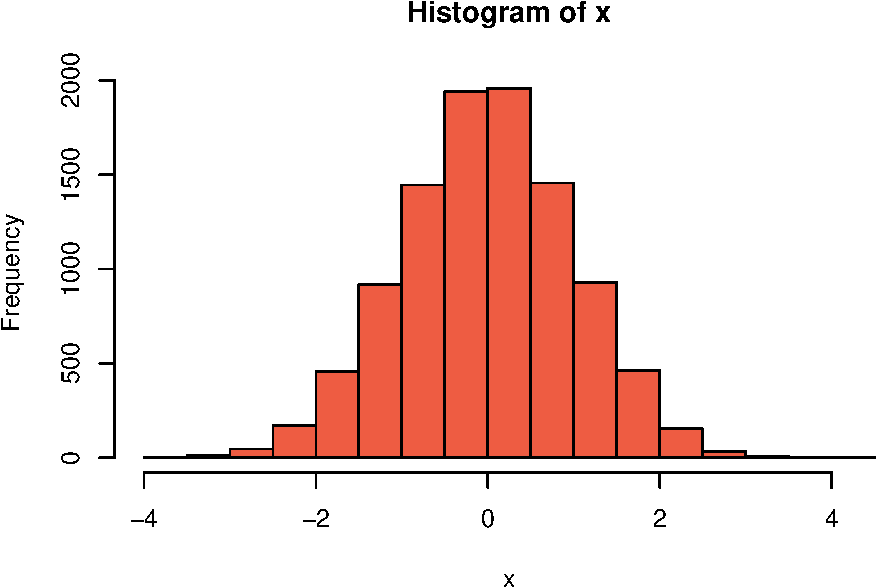
\includegraphics{bookdown-demo_files/figure-latex/unnamed-chunk-76-1.pdf}

\begin{Shaded}
\begin{Highlighting}[]
\FunctionTok{plot}\NormalTok{(x,}\AttributeTok{col=}\StringTok{"salmon"}\NormalTok{) }\CommentTok{\#Gráfica los datos en el orden de aparición en el vector }
\end{Highlighting}
\end{Shaded}

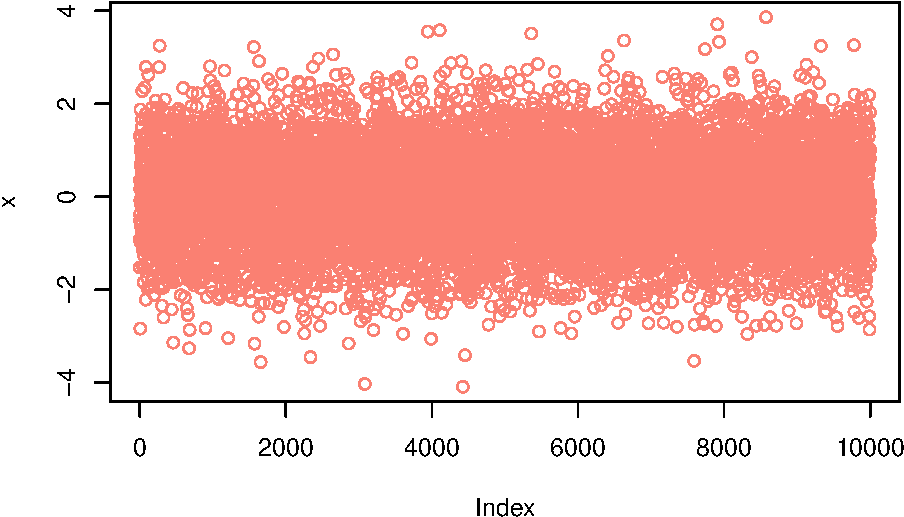
\includegraphics{bookdown-demo_files/figure-latex/unnamed-chunk-76-2.pdf}

\begin{Shaded}
\begin{Highlighting}[]
\FunctionTok{boxplot}\NormalTok{(x,}\AttributeTok{col=}\StringTok{"wheat"}\NormalTok{) }\CommentTok{\#Boxplot: muestra la mediana y quantiles}
\end{Highlighting}
\end{Shaded}

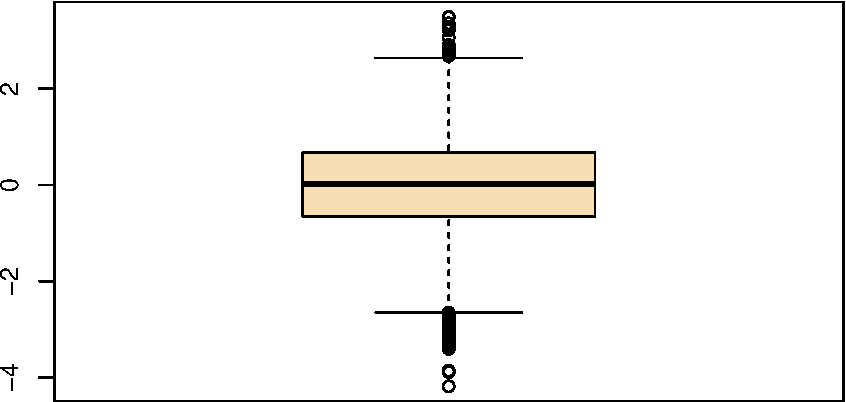
\includegraphics{bookdown-demo_files/figure-latex/unnamed-chunk-76-3.pdf}

\hypertarget{vectores-con-nombre}{%
\section{Vectores con nombre}\label{vectores-con-nombre}}

Una de las cracterísticas de R es que se puede asignar nombres a los vectores, para ello usamos la función \texttt{names()}

Ejemplo:

\begin{Shaded}
\begin{Highlighting}[]
\NormalTok{edades }\OtherTok{\textless{}{-}} \FunctionTok{c}\NormalTok{(}\DecValTok{35}\NormalTok{,}\DecValTok{35}\NormalTok{,}\DecValTok{70}\NormalTok{,}\DecValTok{17}\NormalTok{,}\DecValTok{14}\NormalTok{) }\CommentTok{\#Definimos un vector llamado "edades"}
\NormalTok{nombres }\OtherTok{\textless{}{-}} \FunctionTok{c}\NormalTok{(}\StringTok{"Jerry"}\NormalTok{,}\StringTok{"Beth"}\NormalTok{,}\StringTok{"Rick"}\NormalTok{, }\StringTok{"Summer"}\NormalTok{,}\StringTok{"Morty"}\NormalTok{) }\CommentTok{\#Definimos un vector llamado "edades", del mismo tamaño que "edades"}

\FunctionTok{names}\NormalTok{(edades) }\OtherTok{\textless{}{-}}\NormalTok{ nombres }\CommentTok{\#Se nombran los elementos del vector "edades"}
\NormalTok{edades}
\end{Highlighting}
\end{Shaded}

\begin{verbatim}
##  Jerry   Beth   Rick Summer  Morty 
##     35     35     70     17     14
\end{verbatim}

También se selecciona de la manera usual, por ejemplo, si quiero ver cuál es la edad de Rick, debo seleccionar el elemento 3:

\begin{Shaded}
\begin{Highlighting}[]
\NormalTok{edades[}\DecValTok{3}\NormalTok{]}
\end{Highlighting}
\end{Shaded}

\begin{verbatim}
## Rick 
##   70
\end{verbatim}

Esto es muy poco eficiente y propenso al error, sobre todo con vectores muy grandes. Por ello podemos usar los nombres de los vectores:

\begin{Shaded}
\begin{Highlighting}[]
\NormalTok{edades[}\StringTok{"Rick"}\NormalTok{]}
\end{Highlighting}
\end{Shaded}

\begin{verbatim}
## Rick 
##   70
\end{verbatim}

\textbf{Recuerda que los nombres S-I-E-M-P-R-E van entre comillas}

\begin{Shaded}
\begin{Highlighting}[]
\NormalTok{edades[}\FunctionTok{c}\NormalTok{(}\StringTok{"Rick"}\NormalTok{,}\StringTok{"Morty"}\NormalTok{)]}
\end{Highlighting}
\end{Shaded}

\begin{verbatim}
##  Rick Morty 
##    70    14
\end{verbatim}

\textbf{Ejercicios:}

\begin{enumerate}
\def\labelenumi{\arabic{enumi}.}
\tightlist
\item
  ¿Cuál es el promedio de las edades, sin contar el de Beth?
\item
  Quiten a Morty del vector, ordénenlo y guárdenlo como un nuevo objeto.
\item
  ¿Hay alguna edad que sea mayor de 75? ¿Menor de 12? ¿Entre 12 y 20?
\end{enumerate}

\hypertarget{tamauxf1os-de-genomas}{%
\subsection{Tamaños de genomas}\label{tamauxf1os-de-genomas}}

Ahora veamos un ejemplo más ``biológico''

\begin{Shaded}
\begin{Highlighting}[]
\NormalTok{genomeSizeM\_BP}\OtherTok{\textless{}{-}}\FunctionTok{c}\NormalTok{(}\FloatTok{3234.83}\NormalTok{,}\FloatTok{2716.97}\NormalTok{,}\FloatTok{143.73}\NormalTok{,}\FloatTok{0.014281}\NormalTok{,}\FloatTok{12.1}\NormalTok{)}
\end{Highlighting}
\end{Shaded}

\textbf{NOTA} Si se desea ver el tamaño en bp, simplemente multiplicamos por el valor del prefijo (Mega = 1 millón)

\begin{Shaded}
\begin{Highlighting}[]
\NormalTok{genomeSizeM\_BP}\SpecialCharTok{*}\FloatTok{1e6}
\end{Highlighting}
\end{Shaded}

\begin{verbatim}
## [1] 3234830000 2716970000  143730000      14281   12100000
\end{verbatim}

\begin{Shaded}
\begin{Highlighting}[]
\NormalTok{organismo}\OtherTok{\textless{}{-}}\FunctionTok{c}\NormalTok{(}\StringTok{"Human"}\NormalTok{,}\StringTok{"Mouse"}\NormalTok{,}\StringTok{"Fruit Fly"}\NormalTok{,}\StringTok{"Roundworm"}\NormalTok{,}\StringTok{"Yeast"}\NormalTok{)}
\end{Highlighting}
\end{Shaded}

\begin{Shaded}
\begin{Highlighting}[]
\FunctionTok{names}\NormalTok{(genomeSizeM\_BP)}\OtherTok{\textless{}{-}}\NormalTok{ organismo}
\end{Highlighting}
\end{Shaded}

\begin{Shaded}
\begin{Highlighting}[]
\NormalTok{genomeSizeM\_BP}
\end{Highlighting}
\end{Shaded}

\begin{verbatim}
##       Human       Mouse   Fruit Fly   Roundworm       Yeast 
## 3234.830000 2716.970000  143.730000    0.014281   12.100000
\end{verbatim}

¿Qué hay de diferente entre el primer vector al que le se asiganaron los tamaños de genomas \& esta última versión?

\textbf{RECUERDA}
Se pueden seleccionar elementos de un vector utilizando corchetes:

\begin{Shaded}
\begin{Highlighting}[]
\NormalTok{genomeSizeM\_BP[}\DecValTok{1}\NormalTok{]}
\end{Highlighting}
\end{Shaded}

\begin{verbatim}
##   Human 
## 3234.83
\end{verbatim}

Para obtener elementos consecutivos:

\begin{Shaded}
\begin{Highlighting}[]
\NormalTok{genomeSizeM\_BP[}\DecValTok{1}\SpecialCharTok{:}\DecValTok{4}\NormalTok{]}
\end{Highlighting}
\end{Shaded}

\begin{verbatim}
##       Human       Mouse   Fruit Fly   Roundworm 
## 3234.830000 2716.970000  143.730000    0.014281
\end{verbatim}

Para obtener elementos NO consecutivos:

\begin{Shaded}
\begin{Highlighting}[]
\NormalTok{genomeSizeM\_BP[}\FunctionTok{c}\NormalTok{(}\DecValTok{1}\NormalTok{,}\DecValTok{2}\NormalTok{,}\DecValTok{5}\NormalTok{)]}
\end{Highlighting}
\end{Shaded}

\begin{verbatim}
##   Human   Mouse   Yeast 
## 3234.83 2716.97   12.10
\end{verbatim}

Para descartar (no eliminar, ni quitar) ciertos elementos:

\begin{Shaded}
\begin{Highlighting}[]
\NormalTok{genomeSizeM\_BP[}\SpecialCharTok{{-}}\FunctionTok{c}\NormalTok{(}\DecValTok{1}\NormalTok{,}\DecValTok{3}\NormalTok{,}\DecValTok{5}\NormalTok{)]}
\end{Highlighting}
\end{Shaded}

\begin{verbatim}
##       Mouse   Roundworm 
## 2716.970000    0.014281
\end{verbatim}

Para referirnos a los elementos por el nombre asignado:

\begin{Shaded}
\begin{Highlighting}[]
\NormalTok{genomeSizeM\_BP[}\FunctionTok{c}\NormalTok{(}\StringTok{"Yeast"}\NormalTok{,}\StringTok{"Human"}\NormalTok{)]}
\end{Highlighting}
\end{Shaded}

\begin{verbatim}
##   Yeast   Human 
##   12.10 3234.83
\end{verbatim}

Además de algunas operaciones aritméticas se pueden calcular con la media, máximo, mediana, mínimo, suma y longitud de los vectores

\textbf{Ejercicio}

\begin{enumerate}
\def\labelenumi{\arabic{enumi}.}
\tightlist
\item
  Generar un vector de las edades de 10 de tus compañeros
\item
  Asignales nombre.
\item
  Encuentra el mínimo,máximo, media, mediana, la desviación estándar, la longitud del vector y selecciona sólo los elementos impares.
\item
  Elimina el máximo y el mínimo y con el vector resultante realiza un histograma.
\item
  Crea un vector de caracteres con diez nombres de especies y asocialo con su número de acceso de NCBI para su genoma en nucleótidos.
\end{enumerate}

\hypertarget{cuxf3mo-lidiar-con-las-nas}{%
\section{¿Cómo lidiar con las NAs ?}\label{cuxf3mo-lidiar-con-las-nas}}

Es (muy) freceunte que en bases de datos se tengan valores \texttt{NA}, es decir medidas que no pudieron realizarse, medidas perdidas, etc. Para ello se utiliza \texttt{NA}.
\texttt{R} trata de manera especial a las NAs

\begin{Shaded}
\begin{Highlighting}[]
\NormalTok{x }\OtherTok{\textless{}{-}} \FunctionTok{c}\NormalTok{(}\DecValTok{88}\NormalTok{,}\ConstantTok{NA}\NormalTok{,}\DecValTok{12}\NormalTok{,}\DecValTok{168}\NormalTok{,}\DecValTok{13}\NormalTok{)}
\end{Highlighting}
\end{Shaded}

Existe una fución para determinar si un elemento es o no una \texttt{NA}. La función es \texttt{is.na()}

\begin{Shaded}
\begin{Highlighting}[]
\NormalTok{x }\OtherTok{\textless{}{-}} \FunctionTok{c}\NormalTok{(}\DecValTok{88}\NormalTok{,}\ConstantTok{NA}\NormalTok{,}\DecValTok{12}\NormalTok{,}\DecValTok{168}\NormalTok{,}\DecValTok{13}\NormalTok{)}
\end{Highlighting}
\end{Shaded}

\begin{Shaded}
\begin{Highlighting}[]
\FunctionTok{is.na}\NormalTok{(x)}
\end{Highlighting}
\end{Shaded}

\begin{verbatim}
## [1] FALSE  TRUE FALSE FALSE FALSE
\end{verbatim}

Si queremos calcular ciertas funciones numéricas \texttt{R} no sabrá qué hacer

\begin{Shaded}
\begin{Highlighting}[]
\NormalTok{x }\OtherTok{\textless{}{-}} \FunctionTok{c}\NormalTok{(}\DecValTok{88}\NormalTok{,}\ConstantTok{NA}\NormalTok{,}\DecValTok{12}\NormalTok{,}\DecValTok{168}\NormalTok{,}\DecValTok{13}\NormalTok{)}
\FunctionTok{mean}\NormalTok{(x)}
\end{Highlighting}
\end{Shaded}

\begin{verbatim}
## [1] NA
\end{verbatim}

Sin emabrgo, podemos decirle a \texttt{R} que las omita, indicando como argumento de la función \texttt{mean()} \texttt{na.rm=TRUE} que significa \emph{na remove}

\begin{Shaded}
\begin{Highlighting}[]
\NormalTok{x }\OtherTok{\textless{}{-}} \FunctionTok{c}\NormalTok{(}\DecValTok{88}\NormalTok{,}\ConstantTok{NA}\NormalTok{,}\DecValTok{12}\NormalTok{,}\DecValTok{168}\NormalTok{,}\DecValTok{13}\NormalTok{)}
\FunctionTok{mean}\NormalTok{(x,}\AttributeTok{na.rm=}\ConstantTok{TRUE}\NormalTok{)}
\end{Highlighting}
\end{Shaded}

\begin{verbatim}
## [1] 70.25
\end{verbatim}

¿Qué otras funciones tienen esta opción \texttt{na.rm=TRUE} ?

\hypertarget{filtrado-de-elementos-de-un-vector}{%
\section{Filtrado de elementos de un vector}\label{filtrado-de-elementos-de-un-vector}}

Podemos generar vectores de que sean subconjuntos de vectores más grandes que cumplan cierta(s) condición(es)

\begin{Shaded}
\begin{Highlighting}[]
\NormalTok{un\_vector }\OtherTok{\textless{}{-}} \FunctionTok{c}\NormalTok{(}\DecValTok{1}\NormalTok{,}\DecValTok{2}\NormalTok{,}\DecValTok{3}\NormalTok{,}\DecValTok{5}\NormalTok{,}\DecValTok{7}\NormalTok{,}\DecValTok{11}\NormalTok{,}\DecValTok{13}\NormalTok{,}\DecValTok{17}\NormalTok{,}\DecValTok{19}\NormalTok{) }
\NormalTok{otro\_vector }\OtherTok{\textless{}{-}}\NormalTok{ un\_vector[un\_vector}\SpecialCharTok{*}\NormalTok{un\_vector }\SpecialCharTok{\textgreater{}} \DecValTok{10}\NormalTok{]   }\CommentTok{\#Se lee el vector desde dentro hacía afuera}
\NormalTok{otro\_vector}
\end{Highlighting}
\end{Shaded}

\begin{verbatim}
## [1]  5  7 11 13 17 19
\end{verbatim}

Veamos paso a paso qué es lo que hace este proceso

\begin{Shaded}
\begin{Highlighting}[]
\NormalTok{un\_vector}
\end{Highlighting}
\end{Shaded}

\begin{verbatim}
## [1]  1  2  3  5  7 11 13 17 19
\end{verbatim}

\begin{Shaded}
\begin{Highlighting}[]
\NormalTok{un\_vector}\SpecialCharTok{*}\NormalTok{un\_vector }\SpecialCharTok{\textgreater{}} \DecValTok{10}    \CommentTok{\# Mira, de adentro hacía afuera}
\end{Highlighting}
\end{Shaded}

\begin{verbatim}
## [1] FALSE FALSE FALSE  TRUE  TRUE  TRUE  TRUE  TRUE  TRUE
\end{verbatim}

\begin{Shaded}
\begin{Highlighting}[]
\NormalTok{indices}\OtherTok{\textless{}{-}}\NormalTok{un\_vector}\SpecialCharTok{*}\NormalTok{un\_vector }\SpecialCharTok{\textgreater{}} \DecValTok{10} 
\NormalTok{un\_vector[indices]}
\end{Highlighting}
\end{Shaded}

\begin{verbatim}
## [1]  5  7 11 13 17 19
\end{verbatim}

\begin{Shaded}
\begin{Highlighting}[]
\NormalTok{un\_vector[}\FunctionTok{c}\NormalTok{(}\ConstantTok{FALSE}\NormalTok{,}\ConstantTok{FALSE}\NormalTok{,}\ConstantTok{FALSE}\NormalTok{,}\ConstantTok{TRUE}\NormalTok{,}\ConstantTok{TRUE}\NormalTok{,}\ConstantTok{TRUE}\NormalTok{,}\ConstantTok{TRUE}\NormalTok{,}\ConstantTok{TRUE}\NormalTok{,}\ConstantTok{TRUE}\NormalTok{)]}
\end{Highlighting}
\end{Shaded}

\begin{verbatim}
## [1]  5  7 11 13 17 19
\end{verbatim}

La representación interna de los valores booleanos \texttt{FALSE} y \texttt{TRUE}son 0 y 1, respectivamente

\begin{Shaded}
\begin{Highlighting}[]
\NormalTok{un\_vector[}\FunctionTok{c}\NormalTok{(}\FunctionTok{rep}\NormalTok{(}\DecValTok{0}\NormalTok{,}\DecValTok{3}\NormalTok{),}\FunctionTok{rep}\NormalTok{(}\DecValTok{1}\NormalTok{,}\DecValTok{1}\NormalTok{))]}
\end{Highlighting}
\end{Shaded}

\begin{verbatim}
## [1] 1
\end{verbatim}

\hypertarget{filtrado-con-subset}{%
\subsection{\texorpdfstring{Filtrado con \texttt{subset()}}{Filtrado con subset()}}\label{filtrado-con-subset}}

Podemos usar la función \texttt{subset()}para hacer lo mismo que en el caso anterior \textbf{excepto que omite los NA}

\begin{Shaded}
\begin{Highlighting}[]
\NormalTok{un\_vector}\OtherTok{\textless{}{-}}\FunctionTok{c}\NormalTok{(}\DecValTok{1}\NormalTok{,}\DecValTok{2}\NormalTok{,}\DecValTok{3}\NormalTok{,}\DecValTok{5}\NormalTok{,}\DecValTok{7}\NormalTok{,}\DecValTok{11}\NormalTok{,}\DecValTok{13}\NormalTok{,}\DecValTok{17}\NormalTok{,}\DecValTok{19}\NormalTok{) }
\NormalTok{otro\_vector }\OtherTok{\textless{}{-}} \FunctionTok{subset}\NormalTok{(un\_vector,un\_vector}\SpecialCharTok{*}\NormalTok{un\_vector }\SpecialCharTok{\textgreater{}} \DecValTok{10}\NormalTok{)   }
\NormalTok{otro\_vector}
\end{Highlighting}
\end{Shaded}

\begin{verbatim}
## [1]  5  7 11 13 17 19
\end{verbatim}

Qué pasa si tenemos \texttt{NA}s. Si usamos el método anterior obtendríamos

\begin{Shaded}
\begin{Highlighting}[]
\NormalTok{un\_vector}\OtherTok{\textless{}{-}}\FunctionTok{c}\NormalTok{(}\DecValTok{1}\NormalTok{,}\DecValTok{2}\NormalTok{,}\DecValTok{3}\NormalTok{,}\DecValTok{5}\NormalTok{,}\DecValTok{7}\NormalTok{,}\DecValTok{11}\NormalTok{,}\ConstantTok{NA}\NormalTok{,}\DecValTok{13}\NormalTok{,}\DecValTok{17}\NormalTok{,}\ConstantTok{NA}\NormalTok{,}\DecValTok{19}\NormalTok{) }
\NormalTok{otro\_vector }\OtherTok{\textless{}{-}}\NormalTok{ un\_vector[un\_vector}\SpecialCharTok{*}\NormalTok{un\_vector }\SpecialCharTok{\textgreater{}} \DecValTok{10}\NormalTok{]   }\CommentTok{\# Leeme de adentro hacia afuera}
\NormalTok{otro\_vector  }\CommentTok{\# Aquí salen las NAs}
\end{Highlighting}
\end{Shaded}

\begin{verbatim}
## [1]  5  7 11 NA 13 17 NA 19
\end{verbatim}

En cambio con \texttt{subset()}

\begin{Shaded}
\begin{Highlighting}[]
\NormalTok{un\_vector}\OtherTok{\textless{}{-}}\FunctionTok{c}\NormalTok{(}\DecValTok{1}\NormalTok{,}\DecValTok{2}\NormalTok{,}\DecValTok{3}\NormalTok{,}\DecValTok{5}\NormalTok{,}\DecValTok{7}\NormalTok{,}\DecValTok{11}\NormalTok{,}\ConstantTok{NA}\NormalTok{, }\DecValTok{13}\NormalTok{,}\DecValTok{17}\NormalTok{,}\ConstantTok{NA}\NormalTok{, }\DecValTok{19}\NormalTok{) }
\NormalTok{otro\_vector }\OtherTok{\textless{}{-}} \FunctionTok{subset}\NormalTok{(un\_vector,un\_vector}\SpecialCharTok{*}\NormalTok{un\_vector }\SpecialCharTok{\textgreater{}} \DecValTok{10}\NormalTok{)   }
\NormalTok{otro\_vector  }\CommentTok{\# Aquí ya no aparecen las NAs}
\end{Highlighting}
\end{Shaded}

\begin{verbatim}
## [1]  5  7 11 13 17 19
\end{verbatim}

\hypertarget{la-funciuxf3n-de-selecciuxf3n-which}{%
\subsection{\texorpdfstring{La función de selección \texttt{which()}}{La función de selección which()}}\label{la-funciuxf3n-de-selecciuxf3n-which}}

La función \texttt{which()} nos regresa los índices, es decir, dice \textbf{quiénes} cumplen cierta condición

\begin{Shaded}
\begin{Highlighting}[]
\NormalTok{z }\OtherTok{\textless{}{-}} \FunctionTok{c}\NormalTok{(}\DecValTok{5}\NormalTok{,}\DecValTok{2}\NormalTok{,}\SpecialCharTok{{-}}\DecValTok{3}\NormalTok{,}\DecValTok{8}\NormalTok{)}
\FunctionTok{which}\NormalTok{(z}\SpecialCharTok{*}\NormalTok{z }\SpecialCharTok{\textgreater{}} \DecValTok{8}\NormalTok{)}
\end{Highlighting}
\end{Shaded}

\begin{verbatim}
## [1] 1 3 4
\end{verbatim}

Acá nos dicen quiénes

\begin{Shaded}
\begin{Highlighting}[]
\NormalTok{z[}\FunctionTok{which}\NormalTok{(z}\SpecialCharTok{*}\NormalTok{z }\SpecialCharTok{\textgreater{}} \DecValTok{8}\NormalTok{)]}
\end{Highlighting}
\end{Shaded}

\begin{verbatim}
## [1]  5 -3  8
\end{verbatim}

\hypertarget{cuxf3mo-podemos-ver-si-dos-vectores-son-iguales}{%
\section{¿Cómo podemos ver si dos vectores son iguales?}\label{cuxf3mo-podemos-ver-si-dos-vectores-son-iguales}}

Dos vectores son iguales si elemento a elemento son idénticos.
Por lo tanto deben de ser del mismo tamaño.
\textbf{RECUERDA} Para probar si dos elementos son iguales se utiliza el operador de comparación \texttt{==} son dos signos iguales juntos, sin espacio.
No confundir con el operador \texttt{=} que se puede usar como operador de asiganción (aunque no es recomendable su uso. De hecho está prohibido en este curso \textgreater:(

\begin{Shaded}
\begin{Highlighting}[]
\NormalTok{x }\OtherTok{\textless{}{-}} \FunctionTok{c}\NormalTok{(}\DecValTok{1}\NormalTok{,}\DecValTok{4}\NormalTok{,}\DecValTok{9}\NormalTok{,}\DecValTok{16}\NormalTok{,}\DecValTok{25}\NormalTok{)}
\NormalTok{y }\OtherTok{\textless{}{-}} \DecValTok{1}\SpecialCharTok{:}\DecValTok{5}
\NormalTok{y }\OtherTok{\textless{}{-}}\NormalTok{ y}\SpecialCharTok{*}\NormalTok{y}
\end{Highlighting}
\end{Shaded}

\begin{Shaded}
\begin{Highlighting}[]
\NormalTok{x}\SpecialCharTok{==}\NormalTok{y}
\end{Highlighting}
\end{Shaded}

\begin{verbatim}
## [1] TRUE TRUE TRUE TRUE TRUE
\end{verbatim}

¿Qué pasaría si me confundo y escribo el operador de igualdad en lugar del de comparación?

\begin{Shaded}
\begin{Highlighting}[]
\NormalTok{y }\OtherTok{\textless{}{-}} \DecValTok{5}\SpecialCharTok{:}\DecValTok{9}
\NormalTok{y}
\end{Highlighting}
\end{Shaded}

\begin{verbatim}
## [1] 5 6 7 8 9
\end{verbatim}

\begin{Shaded}
\begin{Highlighting}[]
\NormalTok{x }\OtherTok{=}\NormalTok{ y}
\end{Highlighting}
\end{Shaded}

\begin{Shaded}
\begin{Highlighting}[]
\NormalTok{x}
\end{Highlighting}
\end{Shaded}

\begin{verbatim}
## [1] 5 6 7 8 9
\end{verbatim}

\begin{Shaded}
\begin{Highlighting}[]
\NormalTok{y}
\end{Highlighting}
\end{Shaded}

\begin{verbatim}
## [1] 5 6 7 8 9
\end{verbatim}

Para vectores grandes puedo usar la función \texttt{all()} que ya vimos arriba

\begin{Shaded}
\begin{Highlighting}[]
\NormalTok{x }\OtherTok{\textless{}{-}} \FunctionTok{seq}\NormalTok{(}\DecValTok{1}\NormalTok{,}\DecValTok{10000}\NormalTok{,}\DecValTok{1}\NormalTok{)}
\NormalTok{y }\OtherTok{\textless{}{-}} \FunctionTok{seq}\NormalTok{(}\DecValTok{1}\NormalTok{,}\DecValTok{10000}\NormalTok{,}\DecValTok{1}\NormalTok{)}
\FunctionTok{all}\NormalTok{(x}\SpecialCharTok{==}\NormalTok{y)}
\end{Highlighting}
\end{Shaded}

\begin{verbatim}
## [1] TRUE
\end{verbatim}

¿Cómo podríamos corrobar que son iguales usando \texttt{any}?

También podríamos utilizar que \texttt{TRUE} es \texttt{1} y que \texttt{FALSE} es \texttt{0}

¿Por qué este código nos dice que sí son iguales?

\begin{Shaded}
\begin{Highlighting}[]
\FunctionTok{sum}\NormalTok{(x}\SpecialCharTok{==}\NormalTok{y)}
\end{Highlighting}
\end{Shaded}

\begin{verbatim}
## [1] 10000
\end{verbatim}

\hypertarget{factor}{%
\subsection{Factor}\label{factor}}

Los factores son un tipo de vector que puede tomar un número ``limitado'' de valores, que normalmente se utilizan como variables categóricas. Por ejemplo: macho/hembra. Es útil tenener este tipo de objeto porque varios modelos estadísticos que se pueden correr en \texttt{R} los utilizan. A los valores que pueden tomar los elementos del factor se les conoce como \emph{levels}.

\begin{Shaded}
\begin{Highlighting}[]
\NormalTok{x }\OtherTok{\textless{}{-}} \FunctionTok{c}\NormalTok{(}\DecValTok{1}\NormalTok{,}\DecValTok{2}\NormalTok{,}\DecValTok{2}\NormalTok{,}\DecValTok{3}\NormalTok{,}\DecValTok{1}\NormalTok{,}\DecValTok{2}\NormalTok{,}\DecValTok{3}\NormalTok{,}\DecValTok{3}\NormalTok{,}\DecValTok{1}\NormalTok{,}\DecValTok{2}\NormalTok{,}\DecValTok{3}\NormalTok{,}\DecValTok{3}\NormalTok{,}\DecValTok{1}\NormalTok{)}
\NormalTok{x}
\end{Highlighting}
\end{Shaded}

\begin{verbatim}
##  [1] 1 2 2 3 1 2 3 3 1 2 3 3 1
\end{verbatim}

\begin{Shaded}
\begin{Highlighting}[]
\FunctionTok{as.factor}\NormalTok{(x)}
\end{Highlighting}
\end{Shaded}

\begin{verbatim}
##  [1] 1 2 2 3 1 2 3 3 1 2 3 3 1
## Levels: 1 2 3
\end{verbatim}

\begin{Shaded}
\begin{Highlighting}[]
\NormalTok{x }\OtherTok{\textless{}{-}}\FunctionTok{as.factor}\NormalTok{(x)}
\NormalTok{x}
\end{Highlighting}
\end{Shaded}

\begin{verbatim}
##  [1] 1 2 2 3 1 2 3 3 1 2 3 3 1
## Levels: 1 2 3
\end{verbatim}

Los factores son una manera computacionalmente eficiente de almacenar caracteres, pues cada valor único (\emph{level}) se guarda solo una vez y a los datos se les asigna un valor entero.

\begin{Shaded}
\begin{Highlighting}[]
\NormalTok{meses }\OtherTok{=} \FunctionTok{c}\NormalTok{(}\StringTok{"March"}\NormalTok{,}\StringTok{"April"}\NormalTok{,}\StringTok{"January"}\NormalTok{,}\StringTok{"November"}\NormalTok{,}\StringTok{"January"}\NormalTok{,}
       \StringTok{"September"}\NormalTok{,}\StringTok{"October"}\NormalTok{,}\StringTok{"September"}\NormalTok{,}\StringTok{"November"}\NormalTok{,}\StringTok{"August"}\NormalTok{,}
        \StringTok{"January"}\NormalTok{,}\StringTok{"November"}\NormalTok{,}\StringTok{"November"}\NormalTok{,}\StringTok{"February"}\NormalTok{,}\StringTok{"May"}\NormalTok{,}\StringTok{"August"}\NormalTok{,}
        \StringTok{"July"}\NormalTok{,}\StringTok{"December"}\NormalTok{,}\StringTok{"August"}\NormalTok{,}\StringTok{"August"}\NormalTok{,}\StringTok{"September"}\NormalTok{,}\StringTok{"November"}\NormalTok{,}
         \StringTok{"February"}\NormalTok{,}\StringTok{"April"}\NormalTok{)}
\NormalTok{meses}
\end{Highlighting}
\end{Shaded}

\begin{verbatim}
##  [1] "March"     "April"     "January"   "November"  "January"   "September"
##  [7] "October"   "September" "November"  "August"    "January"   "November" 
## [13] "November"  "February"  "May"       "August"    "July"      "December" 
## [19] "August"    "August"    "September" "November"  "February"  "April"
\end{verbatim}

\begin{Shaded}
\begin{Highlighting}[]
\NormalTok{meses }\OtherTok{\textless{}{-}} \FunctionTok{as.factor}\NormalTok{(meses)}
\NormalTok{meses}
\end{Highlighting}
\end{Shaded}

\begin{verbatim}
##  [1] March     April     January   November  January   September October  
##  [8] September November  August    January   November  November  February 
## [15] May       August    July      December  August    August    September
## [22] November  February  April    
## 11 Levels: April August December February January July March May ... September
\end{verbatim}

El que existan los \emph{levels} permite realizar ciertas operaciones y manipular el contenido del factor.

\begin{Shaded}
\begin{Highlighting}[]
\FunctionTok{table}\NormalTok{(meses)}
\end{Highlighting}
\end{Shaded}

\begin{verbatim}
## meses
##     April    August  December  February   January      July     March 
##         2         4         1         2         3         1         1 
##       May  November   October September 
##         1         5         1         3
\end{verbatim}

\begin{Shaded}
\begin{Highlighting}[]
\FunctionTok{levels}\NormalTok{(meses)}
\end{Highlighting}
\end{Shaded}

\begin{verbatim}
##  [1] "April"     "August"    "December"  "February"  "January"   "July"     
##  [7] "March"     "May"       "November"  "October"   "September"
\end{verbatim}

\begin{Shaded}
\begin{Highlighting}[]
\FunctionTok{levels}\NormalTok{(meses)[}\DecValTok{1}\NormalTok{]}
\end{Highlighting}
\end{Shaded}

\begin{verbatim}
## [1] "April"
\end{verbatim}

\begin{Shaded}
\begin{Highlighting}[]
\FunctionTok{levels}\NormalTok{(meses)[}\DecValTok{1}\NormalTok{]}\OtherTok{\textless{}{-}}\StringTok{"Abril"}
\FunctionTok{levels}\NormalTok{(meses)}
\end{Highlighting}
\end{Shaded}

\begin{verbatim}
##  [1] "Abril"     "August"    "December"  "February"  "January"   "July"     
##  [7] "March"     "May"       "November"  "October"   "September"
\end{verbatim}

\begin{Shaded}
\begin{Highlighting}[]
\NormalTok{meses}
\end{Highlighting}
\end{Shaded}

\begin{verbatim}
##  [1] March     Abril     January   November  January   September October  
##  [8] September November  August    January   November  November  February 
## [15] May       August    July      December  August    August    September
## [22] November  February  Abril    
## 11 Levels: Abril August December February January July March May ... September
\end{verbatim}

\hypertarget{ejercicio-temperaturas-de-incubaciuxf3n}{%
\subsection{Ejercicio: Temperaturas de Incubación}\label{ejercicio-temperaturas-de-incubaciuxf3n}}

Supongamos que estamos realizando un experimento de cultivo bacteriano y registramos las temperaturas de incubación para diferentes muestras. Queremos calcular la temperatura media y la desviación estándar.

\begin{Shaded}
\begin{Highlighting}[]
\CommentTok{\# Temperaturas de incubación (en grados Celsius)}
\NormalTok{temperaturas }\OtherTok{\textless{}{-}} \FunctionTok{c}\NormalTok{(}\DecValTok{37}\NormalTok{, }\DecValTok{37}\NormalTok{, }\DecValTok{25}\NormalTok{, }\DecValTok{30}\NormalTok{, }\DecValTok{30}\NormalTok{, }\DecValTok{37}\NormalTok{, }\DecValTok{25}\NormalTok{, }\DecValTok{25}\NormalTok{)}

\CommentTok{\# Cálculo de la temperatura media}
\NormalTok{temp\_media }\OtherTok{\textless{}{-}} \FunctionTok{mean}\NormalTok{(temperaturas)}
\FunctionTok{cat}\NormalTok{(}\StringTok{"Temperatura media:"}\NormalTok{, temp\_media, }\StringTok{"°C}\SpecialCharTok{\textbackslash{}n}\StringTok{"}\NormalTok{)}
\end{Highlighting}
\end{Shaded}

\begin{verbatim}
## Temperatura media: 30.75 °C
\end{verbatim}

\begin{Shaded}
\begin{Highlighting}[]
\CommentTok{\# Cálculo de la desviación estándar}
\NormalTok{temp\_desviacion }\OtherTok{\textless{}{-}} \FunctionTok{sd}\NormalTok{(temperaturas)}
\FunctionTok{cat}\NormalTok{(}\StringTok{"Desviación estándar:"}\NormalTok{, temp\_desviacion, }\StringTok{"°C}\SpecialCharTok{\textbackslash{}n}\StringTok{"}\NormalTok{)}
\end{Highlighting}
\end{Shaded}

\begin{verbatim}
## Desviación estándar: 5.574175 °C
\end{verbatim}

Supongamos que tenemos un conjunto de temperaturas de incubación de diferentes muestras bacterianas, y queremos identificar las muestras que están dentro de un rango de temperatura óptimo para el crecimiento bacteriano (entre 25°C y 37°C).

\begin{Shaded}
\begin{Highlighting}[]
\CommentTok{\# Vectores con nombre: Muestras y Temperaturas}
\NormalTok{muestras }\OtherTok{\textless{}{-}} \FunctionTok{c}\NormalTok{(}\StringTok{"Muestra1"}\NormalTok{, }\StringTok{"Muestra2"}\NormalTok{, }\StringTok{"Muestra3"}\NormalTok{, }\StringTok{"Muestra4"}\NormalTok{)}
\NormalTok{temperaturas }\OtherTok{\textless{}{-}} \FunctionTok{c}\NormalTok{(}\AttributeTok{Muestra1 =} \DecValTok{37}\NormalTok{, }\AttributeTok{Muestra2 =} \DecValTok{25}\NormalTok{, }\AttributeTok{Muestra3 =} \DecValTok{30}\NormalTok{, }\AttributeTok{Muestra4 =} \DecValTok{40}\NormalTok{)}

\CommentTok{\# Filtrado de temperaturas dentro del rango óptimo}
\NormalTok{temperaturas\_optimas }\OtherTok{\textless{}{-}}\NormalTok{ temperaturas[temperaturas }\SpecialCharTok{\textgreater{}=} \DecValTok{25} \SpecialCharTok{\&}\NormalTok{ temperaturas }\SpecialCharTok{\textless{}=} \DecValTok{37}\NormalTok{]}

\CommentTok{\# Muestras dentro del rango óptimo}
\NormalTok{muestras\_optimas }\OtherTok{\textless{}{-}} \FunctionTok{names}\NormalTok{(temperaturas\_optimas)}

\FunctionTok{cat}\NormalTok{(}\StringTok{"Muestras con temperatura óptima:"}\NormalTok{, muestras\_optimas, }\StringTok{"}\SpecialCharTok{\textbackslash{}n}\StringTok{"}\NormalTok{)}
\end{Highlighting}
\end{Shaded}

\begin{verbatim}
## Muestras con temperatura óptima: Muestra1 Muestra2 Muestra3
\end{verbatim}

\textbf{Ejercicio}
1. Lee la ayuda de \texttt{as.factor} para determinar cómo crear un factor ``ordenado''
2. Crea un vector con los meses en los que todas las alumnas del grupo cumplen años.
3. Aprovecha los levels para generar un objeto que guarde el número de estudiantes que cumplen años cada mes.

\textbf{Ejercicios}

\begin{enumerate}
\def\labelenumi{\arabic{enumi}.}
\tightlist
\item
  Genera un vector con el nombre de 10 virus
\item
  Asocia esos nombres con su número de acceso en NCBI
\item
  Genera otro vector que contega los tamaños en pb y los nombres
\item
  Determina cuáles son mayores de 300 bp
\item
  Asocia un subconjunto de vectores que sean mayores (menores a 300 bp) y mayores (mayores a 300 bp)
\item
  Haz un histograma con los tamaños de todos
\item
  Dibuja un boxplot con los tamaños de todos.Pon en el eje los nombres de todos.
\end{enumerate}

\textbf{Ejercicios adicionales }

\begin{enumerate}
\def\labelenumi{\arabic{enumi}.}
\tightlist
\item
  Crea un vector llamado ``v1'' con los números 2, 4, 6, 8 y 10.
\item
  Crea un vector llamado ``v2'' con los números 1, 3, 5, 7 y 9.
\item
  Suma los vectores ``v1'' y ``v2'' elemento por elemento.
\item
  Multiplica el vector ``v1'' por el escalar 3.
\item
  Calcula la media del vector ``v2''.
\item
  Encuentra el valor mínimo del vector ``v1''.
\item
  Crea un vector llamado ``v3'' con los números 2, 4, 6, 8 y 10.
\item
  Compara los vectores ``v1'' y ``v3'' y determina si son iguales.
\item
  Crea un vector ``v4'' con los primeros 10 números impares.
\item
  Encuentra los elementos comunes entre los vectores ``v2'' y ``v4''
\item
  Crea un vector llamado ``v1'' con números aleatorios enteros entre 1 y 50.
\item
  Ordena el vector ``v1'' de forma descendente.
\item
  Encuentra la mediana del vector ``v1''.
\item
  Crea un vector llamado ``v2'' con números aleatorios enteros entre 10 y 20, de longitud 5.
  15 .Calcula el producto punto entre ``v1'' y ``v2''.
  16 .Crea un vector llamado ``v3'' con números aleatorios entre 0 y 1, de longitud 10.
\item
  Normaliza el vector ``v3''.
\end{enumerate}

\hypertarget{matrices}{%
\chapter{Matrices}\label{matrices}}

Una matriz es un arreglo rectangular de datos del mismo tipo. \textbf{Solo del mismo tipo}. Está compuesta tanto de columnas como de renglones.

\hypertarget{creaciuxf3n-de-matrices}{%
\section{Creación de matrices}\label{creaciuxf3n-de-matrices}}

Para crear una matriz podemos usar la función \texttt{matrix()}. Dicha función requiere de, al menos, un vector e indicar al menos una dimensión.

Ejemplo:

\begin{Shaded}
\begin{Highlighting}[]
\NormalTok{y }\OtherTok{\textless{}{-}} \FunctionTok{matrix}\NormalTok{(}\FunctionTok{c}\NormalTok{(}\DecValTok{1}\NormalTok{,}\DecValTok{5}\NormalTok{,}\DecValTok{8}\NormalTok{,}\SpecialCharTok{{-}}\DecValTok{4}\NormalTok{), }\AttributeTok{nrow=}\DecValTok{2}\NormalTok{, }\AttributeTok{ncol=}\DecValTok{2}\NormalTok{) }\CommentTok{\#nrow: indica el número de renglones \& ncol: indica el número de columnas. }
\NormalTok{y}
\end{Highlighting}
\end{Shaded}

\begin{verbatim}
##      [,1] [,2]
## [1,]    1    8
## [2,]    5   -4
\end{verbatim}

Por default, la matriz va agregando los datos por columnas.

\begin{Shaded}
\begin{Highlighting}[]
\NormalTok{z }\OtherTok{\textless{}{-}} \FunctionTok{matrix}\NormalTok{(}\FunctionTok{c}\NormalTok{(}\ConstantTok{TRUE}\NormalTok{, }\ConstantTok{FALSE}\NormalTok{,}\FunctionTok{rep}\NormalTok{(}\FunctionTok{c}\NormalTok{(}\ConstantTok{TRUE}\NormalTok{, }\ConstantTok{FALSE}\NormalTok{),}\DecValTok{3}\NormalTok{)),}\AttributeTok{nrow=}\DecValTok{4}\NormalTok{)}
\NormalTok{z}
\end{Highlighting}
\end{Shaded}

\begin{verbatim}
##       [,1]  [,2]
## [1,]  TRUE  TRUE
## [2,] FALSE FALSE
## [3,]  TRUE  TRUE
## [4,] FALSE FALSE
\end{verbatim}

¿Por qué sólo es necesario indicar una dimensión (renglones)?

También se puede indicar que se cambien el orden de llenado de la matriz, es decir, en lugar de que lo haga por columnas, lo haga por renglones.

\begin{Shaded}
\begin{Highlighting}[]
\NormalTok{m }\OtherTok{\textless{}{-}} \FunctionTok{matrix}\NormalTok{(}\FunctionTok{c}\NormalTok{(}\DecValTok{1}\NormalTok{,}\DecValTok{2}\NormalTok{,}\DecValTok{3}\NormalTok{,}\DecValTok{4}\NormalTok{,}\DecValTok{5}\NormalTok{,}\DecValTok{6}\NormalTok{),}\AttributeTok{nrow=}\DecValTok{2}\NormalTok{,}\AttributeTok{byrow=}\ConstantTok{TRUE}\NormalTok{)}
\NormalTok{m}
\end{Highlighting}
\end{Shaded}

\begin{verbatim}
##      [,1] [,2] [,3]
## [1,]    1    2    3
## [2,]    4    5    6
\end{verbatim}

\hypertarget{dimensiones-de-un-matriz}{%
\section{Dimensiones de un matriz}\label{dimensiones-de-un-matriz}}

La dimensión de una matriz es el número de renglones y de columnas respectivamente. Se puede obtener usando la función \texttt{dim()} de \emph{dimensión}.
\textbf{NOTA}
\texttt{dim()} no se puede emplear en elementos unidemsionales (Ej: vectores)

\begin{Shaded}
\begin{Highlighting}[]
\FunctionTok{dim}\NormalTok{(y)}
\end{Highlighting}
\end{Shaded}

\begin{verbatim}
## [1] 2 2
\end{verbatim}

\begin{Shaded}
\begin{Highlighting}[]
\FunctionTok{dim}\NormalTok{(z)}
\end{Highlighting}
\end{Shaded}

\begin{verbatim}
## [1] 4 2
\end{verbatim}

Así una matriz se distingue de un vector ya que tiene, además de renglones, columnas.

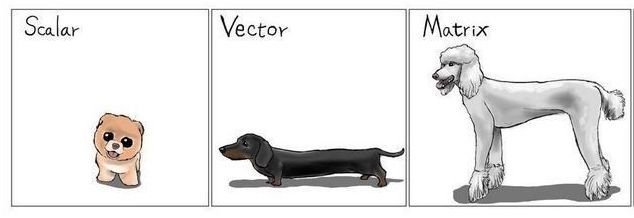
\includegraphics{Escalar_Vector_Matriz.jpeg}
\#\# Elementos de una matriz

Para acceder a elementos de un objeto con \emph{indices} (componentes que tienen una posición asignada), debemos usar \emph{corchetes} \texttt{{[}{]}}. En el caso de la matriz se debe indicar la posición de ambas dimensiones \texttt{{[}renglón,columna{]}}.

Ejemplo: En este caso se desea seleccionar el elemento del primer renglón, segunda columna.

\begin{Shaded}
\begin{Highlighting}[]
\NormalTok{y[}\DecValTok{1}\NormalTok{,}\DecValTok{2}\NormalTok{]}
\end{Highlighting}
\end{Shaded}

\begin{verbatim}
## [1] 8
\end{verbatim}

Ejemplo: En este caso se quiere seleccionar todos los elementos del primer renglón.

\begin{Shaded}
\begin{Highlighting}[]
\NormalTok{y[}\DecValTok{1}\NormalTok{,]}
\end{Highlighting}
\end{Shaded}

\begin{verbatim}
## [1] 1 8
\end{verbatim}

Ejemplo: En este caso se quiere seleccionar todos los elementos de la segunda columna.

\begin{Shaded}
\begin{Highlighting}[]
\NormalTok{y[,}\DecValTok{2}\NormalTok{]}
\end{Highlighting}
\end{Shaded}

\begin{verbatim}
## [1]  8 -4
\end{verbatim}

\hypertarget{creaciuxf3n-de-matriz-vacia}{%
\section{Creación de matriz ``vacia''}\label{creaciuxf3n-de-matriz-vacia}}

Una forma \textbf{mucho menos eficiente} de definir una matriz es declarando una matriz sin elementos (matriz vacía) y después llenándolos de forma explícita asignando un valor distinto a cada posición.

\begin{Shaded}
\begin{Highlighting}[]
\NormalTok{ y }\OtherTok{\textless{}{-}} \FunctionTok{matrix}\NormalTok{(}\AttributeTok{nrow=}\DecValTok{2}\NormalTok{,}\AttributeTok{ncol=}\DecValTok{2}\NormalTok{)}
\NormalTok{y[}\DecValTok{1}\NormalTok{,}\DecValTok{1}\NormalTok{] }\OtherTok{\textless{}{-}} \StringTok{"Esta"}
\NormalTok{y[}\DecValTok{2}\NormalTok{,}\DecValTok{1}\NormalTok{] }\OtherTok{\textless{}{-}} \StringTok{"es"}
\NormalTok{y[}\DecValTok{1}\NormalTok{,}\DecValTok{2}\NormalTok{] }\OtherTok{\textless{}{-}} \StringTok{"una"}
\NormalTok{y[}\DecValTok{2}\NormalTok{,}\DecValTok{2}\NormalTok{] }\OtherTok{\textless{}{-}} \StringTok{"matriz"}
\NormalTok{y}
\end{Highlighting}
\end{Shaded}

\begin{verbatim}
##      [,1]   [,2]    
## [1,] "Esta" "una"   
## [2,] "es"   "matriz"
\end{verbatim}

\hypertarget{operaciones-rbind-y-cbind-en-r-para-matrices}{%
\chapter{Operaciones rbind y cbind en R para Matrices}\label{operaciones-rbind-y-cbind-en-r-para-matrices}}

En R, las funciones \texttt{rbind()} y \texttt{cbind()} se utilizan para unir matrices por filas y columnas, respectivamente. Además, la función \texttt{t()} se utiliza para transponer una matriz.

\hypertarget{uso-de-rbind-para-unir-matrices-por-filas}{%
\section{\texorpdfstring{Uso de \texttt{rbind()} para unir matrices por filas}{Uso de rbind() para unir matrices por filas}}\label{uso-de-rbind-para-unir-matrices-por-filas}}

La función \texttt{rbind()} se utiliza para unir matrices por filas. Por ejemplo, considera las siguientes dos matrices:

\begin{Shaded}
\begin{Highlighting}[]
\CommentTok{\# Matrices de ejemplo}
\NormalTok{matriz1 }\OtherTok{\textless{}{-}} \FunctionTok{matrix}\NormalTok{(}\DecValTok{1}\SpecialCharTok{:}\DecValTok{6}\NormalTok{, }\AttributeTok{nrow =} \DecValTok{2}\NormalTok{)}
\NormalTok{matriz2 }\OtherTok{\textless{}{-}} \FunctionTok{matrix}\NormalTok{(}\DecValTok{7}\SpecialCharTok{:}\DecValTok{12}\NormalTok{, }\AttributeTok{nrow =} \DecValTok{2}\NormalTok{)}

\CommentTok{\# Unir matrices por filas}
\NormalTok{matriz\_unida }\OtherTok{\textless{}{-}} \FunctionTok{rbind}\NormalTok{(matriz1, matriz2)}
\NormalTok{matriz\_unida}
\end{Highlighting}
\end{Shaded}

\begin{verbatim}
##      [,1] [,2] [,3]
## [1,]    1    3    5
## [2,]    2    4    6
## [3,]    7    9   11
## [4,]    8   10   12
\end{verbatim}

\hypertarget{uso-de-cbind-para-unir-matrices-por-columnas}{%
\section{Uso de cbind() para unir matrices por columnas}\label{uso-de-cbind-para-unir-matrices-por-columnas}}

La función cbind() se utiliza para unir matrices por columnas. A continuación, se muestra un ejemplo de cómo unir dos matrices por columnas:

\begin{Shaded}
\begin{Highlighting}[]
\CommentTok{\# Unir matrices por columnas}
\NormalTok{matriz\_unida\_columnas }\OtherTok{\textless{}{-}} \FunctionTok{cbind}\NormalTok{(matriz1, matriz2)}
\NormalTok{matriz\_unida\_columnas}
\end{Highlighting}
\end{Shaded}

\begin{verbatim}
##      [,1] [,2] [,3] [,4] [,5] [,6]
## [1,]    1    3    5    7    9   11
## [2,]    2    4    6    8   10   12
\end{verbatim}

\textbf{Ejercicio}

¿Cómo se llenaría una matriz vacia a partir de vectores?
¿El vector tendría que tener la misma longitud que la columna o el renglón de la matriz?
¿Qué pasaría si la longitud del vector es diferente a la columna o renglón de la matriz?
¿Cómo podrías emplear \texttt{cbind()} \& \texttt{rbind()}?{}`

\hypertarget{operaciones-con-matrices}{%
\section{Operaciones con matrices}\label{operaciones-con-matrices}}

\hypertarget{multiplicaciuxf3n-de-un-escalar-con-una-matriz}{%
\subsection{Multiplicación de un escalar con una matriz}\label{multiplicaciuxf3n-de-un-escalar-con-una-matriz}}

\begin{Shaded}
\begin{Highlighting}[]
\DecValTok{3}\SpecialCharTok{*}\NormalTok{m}
\end{Highlighting}
\end{Shaded}

\begin{verbatim}
##      [,1] [,2] [,3]
## [1,]    3    6    9
## [2,]   12   15   18
\end{verbatim}

\hypertarget{suma-de-dos-matrices}{%
\subsection{Suma de dos matrices}\label{suma-de-dos-matrices}}

\begin{Shaded}
\begin{Highlighting}[]
\NormalTok{m }\SpecialCharTok{+}\NormalTok{ m}
\end{Highlighting}
\end{Shaded}

\begin{verbatim}
##      [,1] [,2] [,3]
## [1,]    2    4    6
## [2,]    8   10   12
\end{verbatim}

\begin{Shaded}
\begin{Highlighting}[]
\NormalTok{n}\OtherTok{\textless{}{-}}\FunctionTok{matrix}\NormalTok{(}\FunctionTok{c}\NormalTok{(}\DecValTok{2}\NormalTok{,}\DecValTok{3}\NormalTok{,}\DecValTok{4}\NormalTok{,}\DecValTok{5}\NormalTok{,}\DecValTok{6}\NormalTok{,}\DecValTok{7}\NormalTok{),}\AttributeTok{ncol=}\DecValTok{3}\NormalTok{)}
\NormalTok{m}\SpecialCharTok{+}\NormalTok{n}
\end{Highlighting}
\end{Shaded}

\begin{verbatim}
##      [,1] [,2] [,3]
## [1,]    3    6    9
## [2,]    7   10   13
\end{verbatim}

Para sumar matrices deben tener las mismas dimensiones

\begin{Shaded}
\begin{Highlighting}[]
\FunctionTok{dim}\NormalTok{(n)}
\end{Highlighting}
\end{Shaded}

\begin{verbatim}
## [1] 2 3
\end{verbatim}

\begin{Shaded}
\begin{Highlighting}[]
\FunctionTok{dim}\NormalTok{(m)}
\end{Highlighting}
\end{Shaded}

\begin{verbatim}
## [1] 2 3
\end{verbatim}

\begin{Shaded}
\begin{Highlighting}[]
\NormalTok{(}\FunctionTok{dim}\NormalTok{(n)}\SpecialCharTok{{-}}\FunctionTok{dim}\NormalTok{(m))}\SpecialCharTok{==}\DecValTok{0}
\end{Highlighting}
\end{Shaded}

\begin{verbatim}
## [1] TRUE TRUE
\end{verbatim}

\hypertarget{multiplicaciuxf3n-de-matrices}{%
\subsection{Multiplicación de matrices}\label{multiplicaciuxf3n-de-matrices}}

Se utiliza el operador \texttt{\%*\%}. Sí. Son tres caracteres. E incluyen dos \texttt{\%}.
No hay espacios y es un sólo operador .

\begin{Shaded}
\begin{Highlighting}[]
\NormalTok{n}\OtherTok{\textless{}{-}}\FunctionTok{matrix}\NormalTok{(}\FunctionTok{c}\NormalTok{(}\DecValTok{2}\NormalTok{,}\DecValTok{3}\NormalTok{,}\DecValTok{4}\NormalTok{,}\DecValTok{5}\NormalTok{,}\DecValTok{6}\NormalTok{,}\DecValTok{7}\NormalTok{),}\AttributeTok{ncol=}\DecValTok{2}\NormalTok{)}
\NormalTok{n}
\end{Highlighting}
\end{Shaded}

\begin{verbatim}
##      [,1] [,2]
## [1,]    2    5
## [2,]    3    6
## [3,]    4    7
\end{verbatim}

\begin{Shaded}
\begin{Highlighting}[]
\NormalTok{m }\SpecialCharTok{\%*\%}\NormalTok{ n }
\end{Highlighting}
\end{Shaded}

\begin{verbatim}
##      [,1] [,2]
## [1,]   20   38
## [2,]   47   92
\end{verbatim}

¿Recuerdas cuál es el criterio para calcular el producto de matrices?
¿Recuerdas cómo se multiplican dos matrices?

\hypertarget{uso-de-la-funciuxf3n-t-para-transponer-una-matriz}{%
\section{\texorpdfstring{Uso de la función \texttt{t()} para transponer una matriz}{Uso de la función t() para transponer una matriz}}\label{uso-de-la-funciuxf3n-t-para-transponer-una-matriz}}

La función \texttt{t()} se utiliza para transponer una matriz, es decir, intercambiar filas por columnas y viceversa. Veamos un ejemplo:

\begin{Shaded}
\begin{Highlighting}[]
\CommentTok{\# Transponer una matriz}
\NormalTok{matriz\_transpuesta }\OtherTok{\textless{}{-}} \FunctionTok{t}\NormalTok{(matriz\_unida\_columnas)}
\NormalTok{matriz\_transpuesta}
\end{Highlighting}
\end{Shaded}

\begin{verbatim}
##      [,1] [,2]
## [1,]    1    2
## [2,]    3    4
## [3,]    5    6
## [4,]    7    8
## [5,]    9   10
## [6,]   11   12
\end{verbatim}

\hypertarget{seleccionar-elementos-de-matrices}{%
\section{Seleccionar elementos de matrices}\label{seleccionar-elementos-de-matrices}}

Para seleccionar elementos de matrices se hace de forma análoga a vectores, es decir, se utiliza el operador \texttt{{[}{]}}. Sólo que esta vez hay que indicar tanto los renglones como la columna en ese orden

\begin{Shaded}
\begin{Highlighting}[]
\NormalTok{m[}\DecValTok{2}\NormalTok{,}\DecValTok{3}\NormalTok{]  }\CommentTok{\# Este es el segundo renglón tercera columna de m}
\end{Highlighting}
\end{Shaded}

\begin{verbatim}
## [1] 6
\end{verbatim}

\begin{Shaded}
\begin{Highlighting}[]
\NormalTok{n[}\DecValTok{3}\NormalTok{,}\DecValTok{2}\NormalTok{]  }\CommentTok{\# Este es el elemento que está en el renglón 3 y columna 2 de la matriz n }
\end{Highlighting}
\end{Shaded}

\begin{verbatim}
## [1] 7
\end{verbatim}

\hypertarget{seleccionar-todoa-una-rengluxf3ncolumna}{%
\subsection{Seleccionar todo(a) un(a) renglón(columna)}\label{seleccionar-todoa-una-rengluxf3ncolumna}}

Para seleccionar todos los elementos de un renglón dado se utiliza la siguiente sintáxis

\begin{Shaded}
\begin{Highlighting}[]
\NormalTok{m[}\DecValTok{2}\NormalTok{,]  }\CommentTok{\# Todos los elementos que están en el segundo renglón}
\end{Highlighting}
\end{Shaded}

\begin{verbatim}
## [1] 4 5 6
\end{verbatim}

Para una columna

\begin{Shaded}
\begin{Highlighting}[]
\NormalTok{m[,}\DecValTok{3}\NormalTok{] }\CommentTok{\# Toda la tercera columna}
\end{Highlighting}
\end{Shaded}

\begin{verbatim}
## [1] 3 6
\end{verbatim}

\hypertarget{selecccionar-elementos-de-una-matriz}{%
\subsection{Selecccionar elementos de una matriz}\label{selecccionar-elementos-de-una-matriz}}

¿Qué hace lo siguiente?

\begin{Shaded}
\begin{Highlighting}[]
\NormalTok{m[}\DecValTok{1}\SpecialCharTok{:}\DecValTok{2}\NormalTok{,}\DecValTok{1}\NormalTok{]}
\end{Highlighting}
\end{Shaded}

\begin{verbatim}
## [1] 1 4
\end{verbatim}

\begin{Shaded}
\begin{Highlighting}[]
\NormalTok{m[}\DecValTok{1}\SpecialCharTok{:}\DecValTok{2}\NormalTok{,}\DecValTok{2}\SpecialCharTok{:}\DecValTok{3}\NormalTok{]}
\end{Highlighting}
\end{Shaded}

\begin{verbatim}
##      [,1] [,2]
## [1,]    2    3
## [2,]    5    6
\end{verbatim}

\begin{Shaded}
\begin{Highlighting}[]
\NormalTok{m[}\SpecialCharTok{{-}}\DecValTok{1}\NormalTok{,]}
\end{Highlighting}
\end{Shaded}

\begin{verbatim}
## [1] 4 5 6
\end{verbatim}

\begin{Shaded}
\begin{Highlighting}[]
\NormalTok{m[}\SpecialCharTok{{-}}\DecValTok{1}\NormalTok{,}\SpecialCharTok{{-}}\FunctionTok{c}\NormalTok{(}\DecValTok{1}\NormalTok{,}\DecValTok{3}\NormalTok{)]}
\end{Highlighting}
\end{Shaded}

\begin{verbatim}
## [1] 5
\end{verbatim}

\hypertarget{nombres-a-renglones-y-columnas}{%
\section{Nombres a renglones y columnas}\label{nombres-a-renglones-y-columnas}}

Al igual que con vectores le podemos poner nombres tanto a renglones como a columnas para ello utilizamos \texttt{rownames()} y \texttt{colnames()}

\begin{Shaded}
\begin{Highlighting}[]
\NormalTok{m   }\CommentTok{\# No tengo nombres :(}
\end{Highlighting}
\end{Shaded}

\begin{verbatim}
##      [,1] [,2] [,3]
## [1,]    1    2    3
## [2,]    4    5    6
\end{verbatim}

\begin{Shaded}
\begin{Highlighting}[]
\FunctionTok{colnames}\NormalTok{(m)}\OtherTok{\textless{}{-}}\NormalTok{LETTERS[}\DecValTok{1}\SpecialCharTok{:}\DecValTok{3}\NormalTok{]}
\FunctionTok{rownames}\NormalTok{(m)}\OtherTok{\textless{}{-}}\NormalTok{letters[}\DecValTok{5}\SpecialCharTok{:}\DecValTok{6}\NormalTok{]}
\end{Highlighting}
\end{Shaded}

\begin{Shaded}
\begin{Highlighting}[]
\NormalTok{m   }\CommentTok{\# Ahora sí. Feos, pero nombres :) :)}
\end{Highlighting}
\end{Shaded}

\begin{verbatim}
##   A B C
## e 1 2 3
## f 4 5 6
\end{verbatim}

\begin{Shaded}
\begin{Highlighting}[]
\NormalTok{m[}\StringTok{"e"}\NormalTok{,}\StringTok{"C"}\NormalTok{]}
\end{Highlighting}
\end{Shaded}

\begin{verbatim}
## [1] 3
\end{verbatim}

\begin{Shaded}
\begin{Highlighting}[]
\NormalTok{m[}\StringTok{"e"}\NormalTok{,}\StringTok{"C"}\NormalTok{]}\SpecialCharTok{==}\NormalTok{m[}\DecValTok{1}\NormalTok{,}\DecValTok{3}\NormalTok{]}
\end{Highlighting}
\end{Shaded}

\begin{verbatim}
## [1] TRUE
\end{verbatim}

\hypertarget{ejercicios}{%
\subsection{Ejercicios}\label{ejercicios}}

\begin{enumerate}
\def\labelenumi{\arabic{enumi}.}
\item
  Genera dos matrices aleatorias de tamaño 3x3 y luego suma ambas matrices.
\item
  Crea dos matrices aleatorias, una de tamaño 2x3 y otra de tamaño 3x4. Luego, calcula su producto matricial.
\item
  Crea una matriz aleatoria de tamaño 4x3 y encuentra su matriz transpuesta.
\item
  Genera una matriz cuadrada aleatoria de tamaño 4x4 y calcula su determinante.
\item
  Crea una matriz cuadrada aleatoria de tamaño 3x3 y encuentra su inversa.
\item
  Genera una matriz aleatoria de tamaño 5x5 y extrae la tercera fila y la segunda columna.
\item
  Crea una matriz diagonal aleatoria de tamaño 4x4 y encuentra sus elementos diagonales.
\item
  Define una matriz de coeficientes A y un vector de términos constantes b. Luego, resuelve el sistema de ecuaciones lineales Ax = b.
\item
  Genera una matriz aleatoria de tamaño 3x3 y multiplica cada uno de sus elementos por un escalar, por ejemplo, 2.
\item
  Crea una matriz simétrica aleatoria de tamaño 4x4 y verifica si es simétrica.
\end{enumerate}

\hypertarget{data-frames}{%
\chapter{Data Frames}\label{data-frames}}

Un Dataframe en R es una estructura de datos rectangular que se compone de filas y columnas, donde cada columna puede tener un tipo de datos diferente. Los Dataframes son una de las estructuras de datos más utilizadas en R, ya que son la forma estándar de almacenar datos tabulares.

\hypertarget{crear-un-dataframe-en-r}{%
\section{Crear un Dataframe en R}\label{crear-un-dataframe-en-r}}

Podemos crear un DataFrame en R utilizando la función \texttt{data.frame()}. Aquí hay un ejemplo de cómo crear un DataFrame simple con datos de estudiantes:

\begin{Shaded}
\begin{Highlighting}[]
\CommentTok{\# Crear un DataFrame de estudiantes}
\NormalTok{estudiantes }\OtherTok{\textless{}{-}} \FunctionTok{data.frame}\NormalTok{(}
  \AttributeTok{nombre =} \FunctionTok{c}\NormalTok{(}\StringTok{"Juan"}\NormalTok{, }\StringTok{"María"}\NormalTok{, }\StringTok{"Pedro"}\NormalTok{, }\StringTok{"Laura"}\NormalTok{),}
  \AttributeTok{edad =} \FunctionTok{c}\NormalTok{(}\DecValTok{20}\NormalTok{, }\DecValTok{22}\NormalTok{, }\DecValTok{21}\NormalTok{, }\DecValTok{23}\NormalTok{),}
  \AttributeTok{puntaje =} \FunctionTok{c}\NormalTok{(}\DecValTok{85}\NormalTok{, }\DecValTok{90}\NormalTok{, }\DecValTok{88}\NormalTok{, }\DecValTok{92}\NormalTok{)}
\NormalTok{)}

\CommentTok{\# Ver el DataFrame}
\FunctionTok{print}\NormalTok{(estudiantes)}
\end{Highlighting}
\end{Shaded}

\begin{verbatim}
##   nombre edad puntaje
## 1   Juan   20      85
## 2  María   22      90
## 3  Pedro   21      88
## 4  Laura   23      92
\end{verbatim}

Para crear un Dataframe en R, puedes utilizar la función \texttt{data.frame()}.
Por ejemplo, para crear un Dataframe con información del genoma de algunos microorganismos, podrías escribir lo siguiente:

\begin{Shaded}
\begin{Highlighting}[]
\NormalTok{dna\_data }\OtherTok{\textless{}{-}} \FunctionTok{data.frame}\NormalTok{(}
  \AttributeTok{secuencia =} \FunctionTok{c}\NormalTok{(}\StringTok{"ATCGATCG"}\NormalTok{, }\StringTok{"GCTAGCTA"}\NormalTok{, }\StringTok{"TTAAGGCT"}\NormalTok{),}
\NormalTok{  tamaño }\OtherTok{=} \FunctionTok{c}\NormalTok{(}\DecValTok{8}\NormalTok{, }\DecValTok{8}\NormalTok{, }\DecValTok{8}\NormalTok{),}
  \AttributeTok{contenido\_GC =} \FunctionTok{c}\NormalTok{(}\FloatTok{0.5}\NormalTok{, }\FloatTok{0.4}\NormalTok{, }\FloatTok{0.3}\NormalTok{)}
\NormalTok{)}

\FunctionTok{print}\NormalTok{(dna\_data)}
\end{Highlighting}
\end{Shaded}

\begin{verbatim}
##   secuencia tamaño contenido_GC
## 1  ATCGATCG      8          0.5
## 2  GCTAGCTA      8          0.4
## 3  TTAAGGCT      8          0.3
\end{verbatim}

\textbf{NOTA} También puedes emplear \texttt{View()} para visualizar el DataFrame.

\begin{Shaded}
\begin{Highlighting}[]
\FunctionTok{View}\NormalTok{(dna\_data)}
\end{Highlighting}
\end{Shaded}

En este ejemplo, el dataframe tiene tres columnas: ``secuencia'', ``tamaño'' y ``contenido\_GC''. La columna ``secuencia'' contiene cadenas de caracteres (strings) que representan las bases del ADN, mientras que las otras dos columnas contienen valores numéricos.

\hypertarget{acceder-a-los-datos-de-un-dataframe}{%
\section{Acceder a los datos de un dataframe}\label{acceder-a-los-datos-de-un-dataframe}}

Para seleccionar elementos o acceder a algún dato de un dataframe, se hace de forma análoga a las matrices, es decir, se utiliza el operador de subíndice \texttt{{[}{]}}.

Por ejemplo, para acceder a la segunda fila de la columna ``secuencia'' en el Dataframe ``dna\_data'', se puede escribir lo siguiente:

\begin{Shaded}
\begin{Highlighting}[]
\NormalTok{dna\_data[}\DecValTok{2}\NormalTok{, }\StringTok{"secuencia"}\NormalTok{]}
\end{Highlighting}
\end{Shaded}

\begin{verbatim}
## [1] "GCTAGCTA"
\end{verbatim}

Esto devolvería la cadena de caracteres ``GCTAGCTA''.

También puedes acceder a varias filas o columnas a la vez.
Por ejemplo, para acceder a las primeras dos filas de las columnas ``tamaño'' y ``contenido\_GC'' en el Dataframe ``dna\_data'', podrías escribir lo siguiente:

\begin{Shaded}
\begin{Highlighting}[]
\NormalTok{dna\_data[}\DecValTok{1}\SpecialCharTok{:}\DecValTok{2}\NormalTok{, }\FunctionTok{c}\NormalTok{(}\StringTok{"tamaño"}\NormalTok{, }\StringTok{"contenido\_GC"}\NormalTok{)]}
\end{Highlighting}
\end{Shaded}

\begin{verbatim}
##   tamaño contenido_GC
## 1      8          0.5
## 2      8          0.4
\end{verbatim}

Esto devolvería un Dataframe con dos filas y dos columnas.

\hypertarget{agregar-y-eliminar-filas-y-columnas-en-un-dataframe-en-r}{%
\section{Agregar y eliminar filas y columnas en un Dataframe en R}\label{agregar-y-eliminar-filas-y-columnas-en-un-dataframe-en-r}}

Para agregar una nueva columna a un Dataframe en R, puedes utilizar el operador de asignación \texttt{\textless{}-}.
Por ejemplo, para agregar una columna que represente la Temperatura de Melting (o Fusión) en el Dataframe ``dna\_data'', podrías escribir lo siguiente:

\begin{Shaded}
\begin{Highlighting}[]
\NormalTok{dna\_data}\SpecialCharTok{$}\NormalTok{temperatura\_melting }\OtherTok{\textless{}{-}} \FunctionTok{c}\NormalTok{(}\DecValTok{24}\NormalTok{, }\DecValTok{24}\NormalTok{, }\DecValTok{20}\NormalTok{)}
\end{Highlighting}
\end{Shaded}

Esto crearía una nueva columna llamada ``temperatura\_melting'' en el Dataframe ``dna\_data'' y la inicializaría con los valores proporcionados.

Para eliminar una columna de un Dataframe en R, puedes utilizar el operador de subíndice\texttt{{[}{]}} con un valor nulo para la columna que deseas eliminar. Por ejemplo, para eliminar la columna ``temperatura\_melting'' del Dataframe ``dna\_data'', podrías escribir lo siguiente:

\begin{Shaded}
\begin{Highlighting}[]
\NormalTok{dna\_data}\SpecialCharTok{$}\NormalTok{temperatura\_melting }\OtherTok{\textless{}{-}} \ConstantTok{NULL}
\end{Highlighting}
\end{Shaded}

Para agregar una nueva fila a un Dataframe en R, puedes utilizar la función \texttt{rbind()}. ¿También se puede aplicar \texttt{cbind()} en Dataframe?

\textbf{Ejercicio}
Empleando la siguiente fórmula para calcular la Temperatura de Fusión: \texttt{Tm=4(G+C)+2(A+T)}, diseña una secuencia que cumpla con una Tm de 55°. Agrega sus características (secuencia, tamaño, cantidad GC \& Tm) en una nueva fila. También será necesario agregar la columna Tm para indicar la Temperatura de Fusión de cada secuencia. Usa el Dataframe \texttt{dna\_data} como base.

\hypertarget{importar-un-archivo-csv-en-r}{%
\chapter{Importar un archivo csv en R}\label{importar-un-archivo-csv-en-r}}

Un archivo csv (Comma Separated Values) es un archivo de texto que contiene datos en formato tabular, donde cada fila representa un registro y cada columna representa una variable. Para importar un archivo CSV en R, puedes utilizar la función \texttt{read.csv()}. Por ejemplo, si tienes un archivo llamado ``ventas.csv'' en tu directorio de trabajo actual, puedes importarlo de la siguiente manera:

\begin{Shaded}
\begin{Highlighting}[]
\CommentTok{\#ventas \textless{}{-} read.csv("ventas.csv")}
\end{Highlighting}
\end{Shaded}

Esto creará un Dataframe llamado ``ventas'' en R, que contendrá los datos del archivo CSV.

Si el archivo CSV utiliza un separador de campos diferente a la coma, puedes utilizar la función read.csv2() en su lugar. Por ejemplo, si el archivo CSV utiliza un punto y coma como separador de campos, puedes importarlo de la siguiente manera:

\begin{Shaded}
\begin{Highlighting}[]
\CommentTok{\#ventas \textless{}{-} read.csv2("ventas.csv")}
\end{Highlighting}
\end{Shaded}

\hypertarget{importar-un-archivo-tsv-en-r}{%
\section{Importar un archivo TSV en R}\label{importar-un-archivo-tsv-en-r}}

Un archivo TSV (Tab Separated Values) es similar a un archivo CSV, pero utiliza \textbf{tabulaciones} en lugar de comas para separar los campos. Para importar un archivo TSV en R, puedes utilizar la función read.delim(). Por ejemplo, si tienes un archivo llamado ``ventas.tsv'' en tu directorio de trabajo actual, puedes importarlo de la siguiente manera:

\begin{Shaded}
\begin{Highlighting}[]
\CommentTok{\#ventas \textless{}{-} read.delim("ventas.tsv")}
\end{Highlighting}
\end{Shaded}

Esto creará un Dataframe llamado ``ventas'' en R, que contendrá los datos del archivo TSV.

Si el archivo TSV utiliza un separador de campos diferente a la tabulación, puedes utilizar la función \texttt{read.delim2()} en su lugar.

\hypertarget{importar-un-archivo-excel-en-r}{%
\section{Importar un archivo Excel en R}\label{importar-un-archivo-excel-en-r}}

Un archivo de Excel es un formato de archivo popular para almacenar datos en formato tabular. Para importar un archivo de Excel en R, puedes utilizar la función readxl::read\_excel() del paquete ``readxl''. Por ejemplo, si tienes un archivo llamado ``ventas.xlsx'' en tu directorio de trabajo actual, puedes importarlo de la siguiente manera:

\begin{Shaded}
\begin{Highlighting}[]
\FunctionTok{library}\NormalTok{(readxl)}
\CommentTok{\#ventas \textless{}{-} read\_excel("ventas.xlsx")}
\end{Highlighting}
\end{Shaded}

\hypertarget{Estructuras_de_seleccion}{%
\chapter{Estructuras de selección}\label{Estructuras_de_seleccion}}

\begin{enumerate}
\def\labelenumi{\arabic{enumi}.}
\tightlist
\item
  \texttt{if}
\item
  \texttt{if} \ldots{} \texttt{else}
\item
  \texttt{ifelse}
\item
  \texttt{if\ ...\ else\ if\ ...else\ if\ ...else}
\end{enumerate}

\hypertarget{if-si-condicional}{%
\section{If (si condicional)}\label{if-si-condicional}}

La instrucción \texttt{if} nos permite probar una condición y esa condición debe arrojar un valor booleano, es decir, un valor de verdad (\texttt{TRUE} o \texttt{FALSE}) Si la condición es verdadera se ejecuta lo que está dentro de los corchetes, de lo contrario, ejecuta lo que sigue después del corchete de cierre.

\textbf{Definición}: Lo que se encuentra dentra del corchete se llama cuerpo ( \emph{body} ) de la declaración \texttt{if}

\begin{figure}
\hypertarget{id}{%
\centering
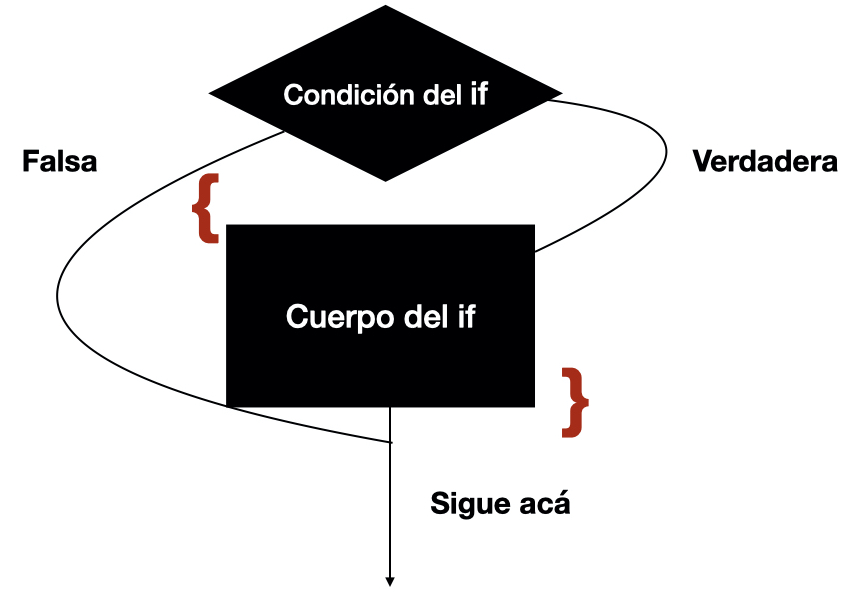
\includegraphics[width=1\textwidth,height=1\textheight]{If_R.001.jpeg}
\caption{Diagrama de flujo del If}\label{id}
}
\end{figure}

La sintaxis de una condición \texttt{if} consiste en lo siguiente:

\texttt{if\ (condicion)\{}

\texttt{si\ la\ condicion\ es\ verdadera}

\texttt{Ejecuta\ TODO\ lo\ que\ está\ en\ los\ corchetes}

\texttt{\}}

\hypertarget{sintaxis}{%
\subsection{Sintaxis}\label{sintaxis}}

\begin{Shaded}
\begin{Highlighting}[]
\ControlFlowTok{if}\NormalTok{(}\SpecialCharTok{\textless{}}\NormalTok{condition}\SpecialCharTok{\textgreater{}}\NormalTok{) \{}
        \DocumentationTok{\#\# Hace algo}
\NormalTok{\} }
\DocumentationTok{\#\# Continúa con el resto del código}
\end{Highlighting}
\end{Shaded}

\hypertarget{errores-comunes-en-el-if}{%
\subsection{\texorpdfstring{Errores comunes en el \texttt{if}}{Errores comunes en el if}}\label{errores-comunes-en-el-if}}

\begin{enumerate}
\def\labelenumi{\arabic{enumi}.}
\tightlist
\item
  No incializar la variable de la condición.
\item
  La condición no arroja un valor de verdad.
\item
  No poner todo lo que quieres que haga \textbf{dentro} de los corchetes.
\item
  Este no es un error, es más bien una advertencia, si la condición arroja un sólo valor de verdad sólo toma en cuenta el primero de ellos.
\end{enumerate}

\#\#\#Ejemplos de uso del \texttt{if}

\begin{Shaded}
\begin{Highlighting}[]
\NormalTok{mayor\_de\_edad}\OtherTok{\textless{}{-}}\DecValTok{18}

\NormalTok{edad}\OtherTok{\textless{}{-}}\DecValTok{20}

\ControlFlowTok{if}\NormalTok{(edad }\SpecialCharTok{\textgreater{}=}\NormalTok{mayor\_de\_edad)\{}
  \FunctionTok{print}\NormalTok{(}\StringTok{"Eres mayor de edad"}\NormalTok{)}
\NormalTok{\}}
\end{Highlighting}
\end{Shaded}

\begin{verbatim}
## [1] "Eres mayor de edad"
\end{verbatim}

\begin{Shaded}
\begin{Highlighting}[]
\NormalTok{x}\OtherTok{\textless{}{-}}\DecValTok{5}\SpecialCharTok{+}\DecValTok{4}
\FunctionTok{print}\NormalTok{(x)}
\end{Highlighting}
\end{Shaded}

\begin{verbatim}
## [1] 9
\end{verbatim}

\begin{Shaded}
\begin{Highlighting}[]
\NormalTok{minimo}\OtherTok{\textless{}{-}}\DecValTok{20000}
\NormalTok{dinero}\OtherTok{\textless{}{-}}\DecValTok{15000}

\ControlFlowTok{if}\NormalTok{(dinero}\SpecialCharTok{\textgreater{}=}\NormalTok{minimo)\{}
  \FunctionTok{print}\NormalTok{(}\StringTok{"¿Cómo está Cancún?"}\NormalTok{)}
  \FunctionTok{print}\NormalTok{(}\StringTok{"La vida es buena"}\NormalTok{)}
\NormalTok{  sobrante}\OtherTok{\textless{}{-}}\NormalTok{dinero}\SpecialCharTok{{-}}\NormalTok{minimo}
  \FunctionTok{print}\NormalTok{(}\FunctionTok{paste}\NormalTok{(}\StringTok{"Me queda $"}\NormalTok{, sobrante))}
\NormalTok{\}}
\FunctionTok{print}\NormalTok{(}\StringTok{"Acá sigue"}\NormalTok{)}
\end{Highlighting}
\end{Shaded}

\begin{verbatim}
## [1] "Acá sigue"
\end{verbatim}

\hypertarget{ejercicios-1}{%
\subsubsection{Ejercicios}\label{ejercicios-1}}

\begin{enumerate}
\def\labelenumi{\arabic{enumi}.}
\tightlist
\item
  Elabora un programa que compare tu estatura con tu ídolx y determine si eres más altx.
\item
  Toma dos archivos fasta de virus distintos. Leelos con Biostrings y compara sus tamaños ( en bp) y determina si el primero es más grande que el segundo.
\item
  A partir del archivo de anotación del genoma de un organismo determina toma dos proteínas al azar y compara sus tamaños. Toma todos los genes de la cadena positiva y todos los de la negativa compara sus tamaños promedio y determina cuál de estos es más grande.
\end{enumerate}

\begin{center}\rule{0.5\linewidth}{0.5pt}\end{center}

\hypertarget{combinaciuxf3n-de-operadores-booleanos}{%
\section{Combinación de operadores booleanos}\label{combinaciuxf3n-de-operadores-booleanos}}

Los operadores lógicos o booleanos se pueden combinar para formar enunciados complejos por ejemplo:

\begin{enumerate}
\def\labelenumi{\arabic{enumi}.}
\tightlist
\item
  Tengo vacaciones (del trabajo y/o la escuela)
\item
  Tengo dinero
\end{enumerate}

Si las dos condiciones son ciertas entonces puedo hacer algo

También podría ser que basta con que una de ellas sea cierta para que haga algo.

\hypertarget{and}{%
\subsection{And (\&)}\label{and}}

El operador booleano \texttt{\&} representa el y lógico. Estos operadores binarios nos sirven para unir al menos dos enunciados que tienen valor de verdadero o falso (Tengo dinero (V/F), Tengo vacaciones (V/F))

Con estas dos operaciones puedo unirlas utilizando el operador \texttt{y} lógico (AND (\texttt{\&}) representado en R con el símbolo del ampersand (\texttt{\&})

Tengo dinero AND Tengo vaciones

Para saber el valor booleano (V/F) del enunciado anterior debemos concocer los valores de verdad de los enunciados por separado

Por ejemplo, podemos representar al primer enunciado por \texttt{p} y al segundo enunciado por \texttt{q}

\texttt{p:\ Tengo\ dinero}

\texttt{q:\ Tengo\ vacaciones}

Para saber cuál es el valor de verdad del enunciado compuesto debemos ver cuáles son todas las combinaciones de valores de verdad de los enunciados que la componen: p verdadero y q verdadero, p falso y q verdadero, p falso y q verdadero, p falso y q falso. Eso se resumen en las tablas de verdad de los operadores

\begin{longtable}[]{@{}ccc@{}}
\caption{Tabla de verdad del AND}\tabularnewline
\toprule\noalign{}
p & q & p \& q \\
\midrule\noalign{}
\endfirsthead
\toprule\noalign{}
p & q & p \& q \\
\midrule\noalign{}
\endhead
\bottomrule\noalign{}
\endlastfoot
V & V & V \\
V & F & F \\
F & V & F \\
F & F & F \\
\end{longtable}

Es decir, el \texttt{\&} solo es \textbf{verdadero} cuando ambas condciones son \textbf{verdaderas}.

Esto representa lo que se observa en la realidad: es decir, solo hago algo si tengo y tengo vacaciones. Si una de ellas no se cumple (es decir, es falsa) entonces no se lleva a cabo la acción.

\hypertarget{or}{%
\subsection{OR (\textbar)}\label{or}}

El operador booleano \texttt{\textbar{}} representa el \texttt{o} lógico. Estos operadores binarios nos sirven para unir al menos dos enunciados que tienen valor de verdadero o falso (Tengo dinero (V/F), Tengo vacaciones (V/F))

Con estas dos operaciones puedo unirlas utilizando el operador \texttt{y} lógico (OR (\texttt{\textbar{}}) representado en R con el símbolo de \emph{la barrita} (\texttt{\textbar{}})

Tengo dinero OR Tengo vaciones

Para saber el valor booleano (V/F) del enunciado anterior debemos concocer los valores de verdad de los enunciados por separado

Por ejmplo podemos representar al primer enunciado por \texttt{p} y al segundo enunciado por \texttt{q}

\texttt{p:\ Tengo\ dinero}

\texttt{q:\ Tengo\ vacaciones}

Para saber cuál es el valor de verdad del enunciado compuesto debemos ver cuáles son todas las combinaciones de valores de verdad de los enunciados que la componen: p verdadero y q verdadero, p falso y q verdadero, p falso y q verdadero, p falso y q falso. Eso se resumen en las tablas de verdad de los operadores

\begin{longtable}[]{@{}ccc@{}}
\caption{Tabla de verdad del operador OR}\tabularnewline
\toprule\noalign{}
p & q & p \textbar{} q \\
\midrule\noalign{}
\endfirsthead
\toprule\noalign{}
p & q & p \textbar{} q \\
\midrule\noalign{}
\endhead
\bottomrule\noalign{}
\endlastfoot
V & V & V \\
V & F & V \\
F & V & V \\
F & F & F \\
\end{longtable}

Es decir haría algo, por ejemplo, irme a la playa cuando \textbf{al menos} una condición se cumpla. Por ejemplo que tenga dinero aunque no tenga vacaciones, que tenga vacaciones aunque no tenga dinero y, obviamente, también cuando las dos se cumplen.

Es decir, el \texttt{\textbar{}} solo es \textbf{falso} cuando ambas condiciones son \textbf{falsas}.

\hypertarget{ejemplos-de-combinaciones}{%
\subsection{Ejemplos de combinaciones}\label{ejemplos-de-combinaciones}}

Por eejmplo es útil para intervalos

\[
18 \leq edad \leq 29 
\]

Esta condición la podemos expresar mediante la combinación de dos: la edad debe ser mayor igual a 18 y (\textbf{AND}, \texttt{\&}) la edad debe ser menor o igual que 29

\begin{Shaded}
\begin{Highlighting}[]
\ControlFlowTok{if}\NormalTok{ (edad }\SpecialCharTok{\textgreater{}=} \DecValTok{18} \SpecialCharTok{\&}\NormalTok{ edad }\SpecialCharTok{\textless{}=}\DecValTok{29}\NormalTok{)\{}
  \FunctionTok{print}\NormalTok{(}\StringTok{"Te toca vacunarte"}\NormalTok{)}
\NormalTok{\}}
\end{Highlighting}
\end{Shaded}

\begin{verbatim}
## [1] "Te toca vacunarte"
\end{verbatim}

\textbf{Pregunta}: ¿qué pasaría si se pone un \textbf{OR} como unión entre las dos condiciones

\begin{Shaded}
\begin{Highlighting}[]
\ControlFlowTok{if}\NormalTok{ (edad }\SpecialCharTok{\textgreater{}=} \DecValTok{18} \SpecialCharTok{|}\NormalTok{ edad }\SpecialCharTok{\textless{}=}\DecValTok{29}\NormalTok{)\{}
  \FunctionTok{print}\NormalTok{(}\StringTok{"Te toca vacunarte"}\NormalTok{)}
\NormalTok{\}}
\end{Highlighting}
\end{Shaded}

\begin{verbatim}
## [1] "Te toca vacunarte"
\end{verbatim}

o así (¿es lo mismo?)

\begin{Shaded}
\begin{Highlighting}[]
\ControlFlowTok{if}\NormalTok{ (edad }\SpecialCharTok{\textless{}=} \DecValTok{29} \SpecialCharTok{|}\NormalTok{ edad }\SpecialCharTok{\textgreater{}=} \DecValTok{18}\NormalTok{)\{}
  \FunctionTok{print}\NormalTok{(}\StringTok{"Te toca vacunarte"}\NormalTok{)}
\NormalTok{\}}
\end{Highlighting}
\end{Shaded}

\begin{verbatim}
## [1] "Te toca vacunarte"
\end{verbatim}

\hypertarget{ejercicio}{%
\section{Ejercicio}\label{ejercicio}}

\begin{enumerate}
\def\labelenumi{\arabic{enumi}.}
\item
  ¿Cómo harías una condición que considere que te gusta el mole y el pozole?
\item
  ¿Cómo harías una condición que considere que te gusta el mole o el pozole?
\end{enumerate}

\hypertarget{if-else-si-de-otro-modo}{%
\section{If \ldots{} else (si \ldots{} de otro modo)}\label{if-else-si-de-otro-modo}}

Si además quieres que se ejecute algo cuando la condición es \textbf{falsa} entonces debes usar la declaración \texttt{if\ …\ else}

\begin{Shaded}
\begin{Highlighting}[]
\ControlFlowTok{if}\NormalTok{ (condición) \{ }\CommentTok{\# Si la condición es cierta}
\NormalTok{hace esto}
\NormalTok{y esto}
\NormalTok{y esto}
\NormalTok{\} }\ControlFlowTok{else}\NormalTok{ \{ }\CommentTok{\# De otro modo, es decir si es falsa hace lo que \#está en el corchete}
\NormalTok{entonces hace esto otro}
\NormalTok{y esto otro}
\NormalTok{y esto}
\NormalTok{\}}
\end{Highlighting}
\end{Shaded}

\begin{figure}
\hypertarget{id}{%
\centering
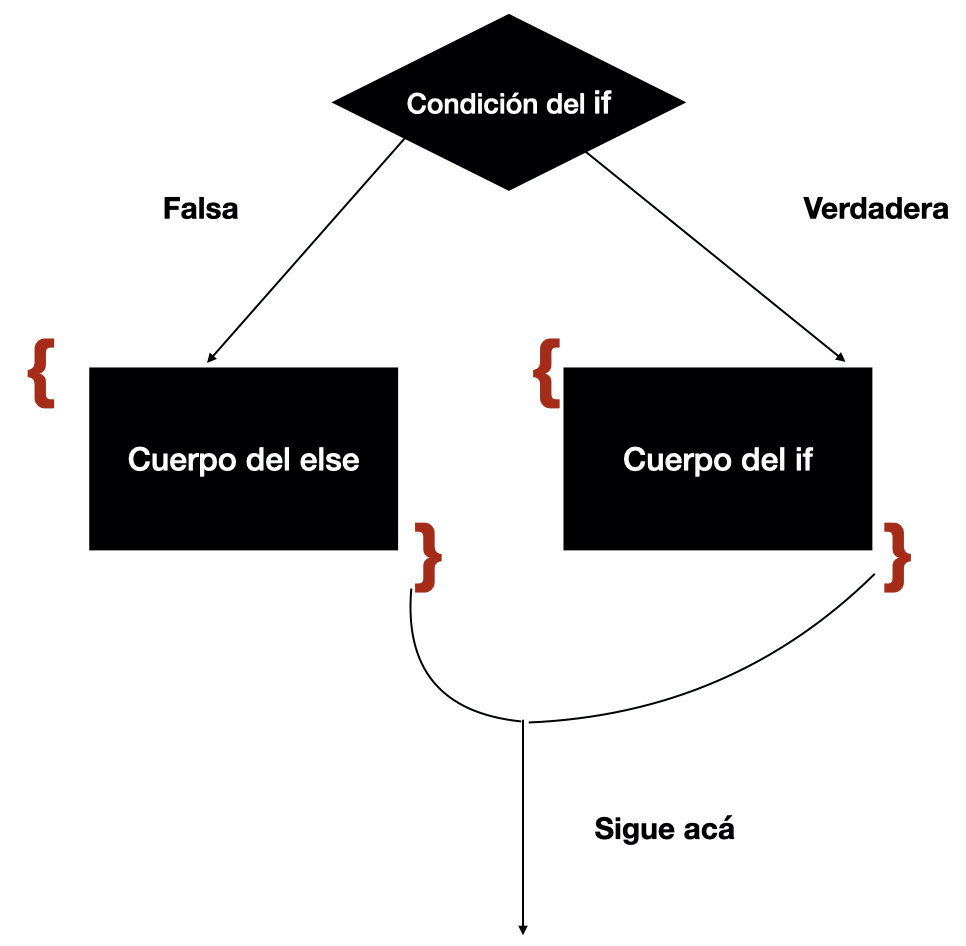
\includegraphics[width=1\textwidth,height=1\textheight]{If_else.001.jpeg}
\caption{Diagrama\_if\_else}\label{id}
}
\end{figure}

\begin{Shaded}
\begin{Highlighting}[]
\NormalTok{minimo}\OtherTok{\textless{}{-}}\DecValTok{20000}
\NormalTok{vacaciones}\OtherTok{\textless{}{-}}\StringTok{"SI"}
\NormalTok{dinero}\OtherTok{\textless{}{-}}\DecValTok{21000}
\ControlFlowTok{if}\NormalTok{(dinero}\SpecialCharTok{\textgreater{}=}\NormalTok{minimo }\SpecialCharTok{\&}\NormalTok{ vacaciones}\SpecialCharTok{==}\StringTok{"SI"}\NormalTok{)\{}
  \FunctionTok{print}\NormalTok{(}\StringTok{"Me voy a la playa, looser"}\NormalTok{)}
\NormalTok{\}}\ControlFlowTok{else}\NormalTok{\{}
  \FunctionTok{print}\NormalTok{(}\StringTok{"Me quedo en mi casa"}\NormalTok{)}
\NormalTok{\}}
\end{Highlighting}
\end{Shaded}

\begin{verbatim}
## [1] "Me voy a la playa, looser"
\end{verbatim}

\hypertarget{ifelse}{%
\section{ifelse}\label{ifelse}}

Si la condición es muy simple ,tanto para cuando es verdadero como cuando es falso se puede implementar la función \texttt{ifelse} en una línea. Es equivalente a la condición compuesta pero ahorramos código.

\begin{Shaded}
\begin{Highlighting}[]
\NormalTok{edad}\OtherTok{\textless{}{-}}\DecValTok{21}
\FunctionTok{ifelse}\NormalTok{(edad}\SpecialCharTok{\textgreater{}=}\DecValTok{18}\NormalTok{, }\StringTok{"Ya eres grande"}\NormalTok{,}\StringTok{"Todavia no puedes beber (legalmente)"}\NormalTok{)}
\end{Highlighting}
\end{Shaded}

\begin{verbatim}
## [1] "Ya eres grande"
\end{verbatim}

\begin{Shaded}
\begin{Highlighting}[]
\NormalTok{edad}\OtherTok{\textless{}{-}}\DecValTok{12}
\FunctionTok{ifelse}\NormalTok{(edad}\SpecialCharTok{\textgreater{}=}\DecValTok{18}\NormalTok{, }\StringTok{"Ya eres grande"}\NormalTok{,}\StringTok{"Todavia no puedes beber (legalmente)"}\NormalTok{)}
\end{Highlighting}
\end{Shaded}

\begin{verbatim}
## [1] "Todavia no puedes beber (legalmente)"
\end{verbatim}

\hypertarget{if-else-if-else-si-si-no-si-si-no-si-si-no}{%
\section{If \ldots{} else if \ldots{} else ( si, si no si , si no si, si no)}\label{if-else-if-else-si-si-no-si-si-no-si-si-no}}

Si tienes más opciones, es decir no alternativas, puedes usar la sentencia \texttt{if\ …\ else\ if\ …else\ if\ …else}

\begin{description}
\item[Importante]
Esta estructura se ejecuta solo en la primera que sea verdadera o si no hay una verdadera ejecuta lo que esta en el \texttt{else}
\end{description}

\begin{Shaded}
\begin{Highlighting}[]
\ControlFlowTok{if}\NormalTok{ ( condicion }\DecValTok{1}\NormalTok{) \{}
\NormalTok{Hace cosas}
\NormalTok{\} }\ControlFlowTok{else} \ControlFlowTok{if}\NormalTok{ ( condcion }\DecValTok{2}\NormalTok{) \{}
\NormalTok{Hace otras cosas}
\NormalTok{\} }\ControlFlowTok{else} \ControlFlowTok{if}\NormalTok{ ( condicion }\DecValTok{3}\NormalTok{) \{}
\NormalTok{Hace estas otras cosas}
\NormalTok{\} }\ControlFlowTok{else}\NormalTok{ \{}
\NormalTok{No le queda de otra y hace esto}
\NormalTok{\}}
\end{Highlighting}
\end{Shaded}

\begin{figure}
\hypertarget{id}{%
\centering
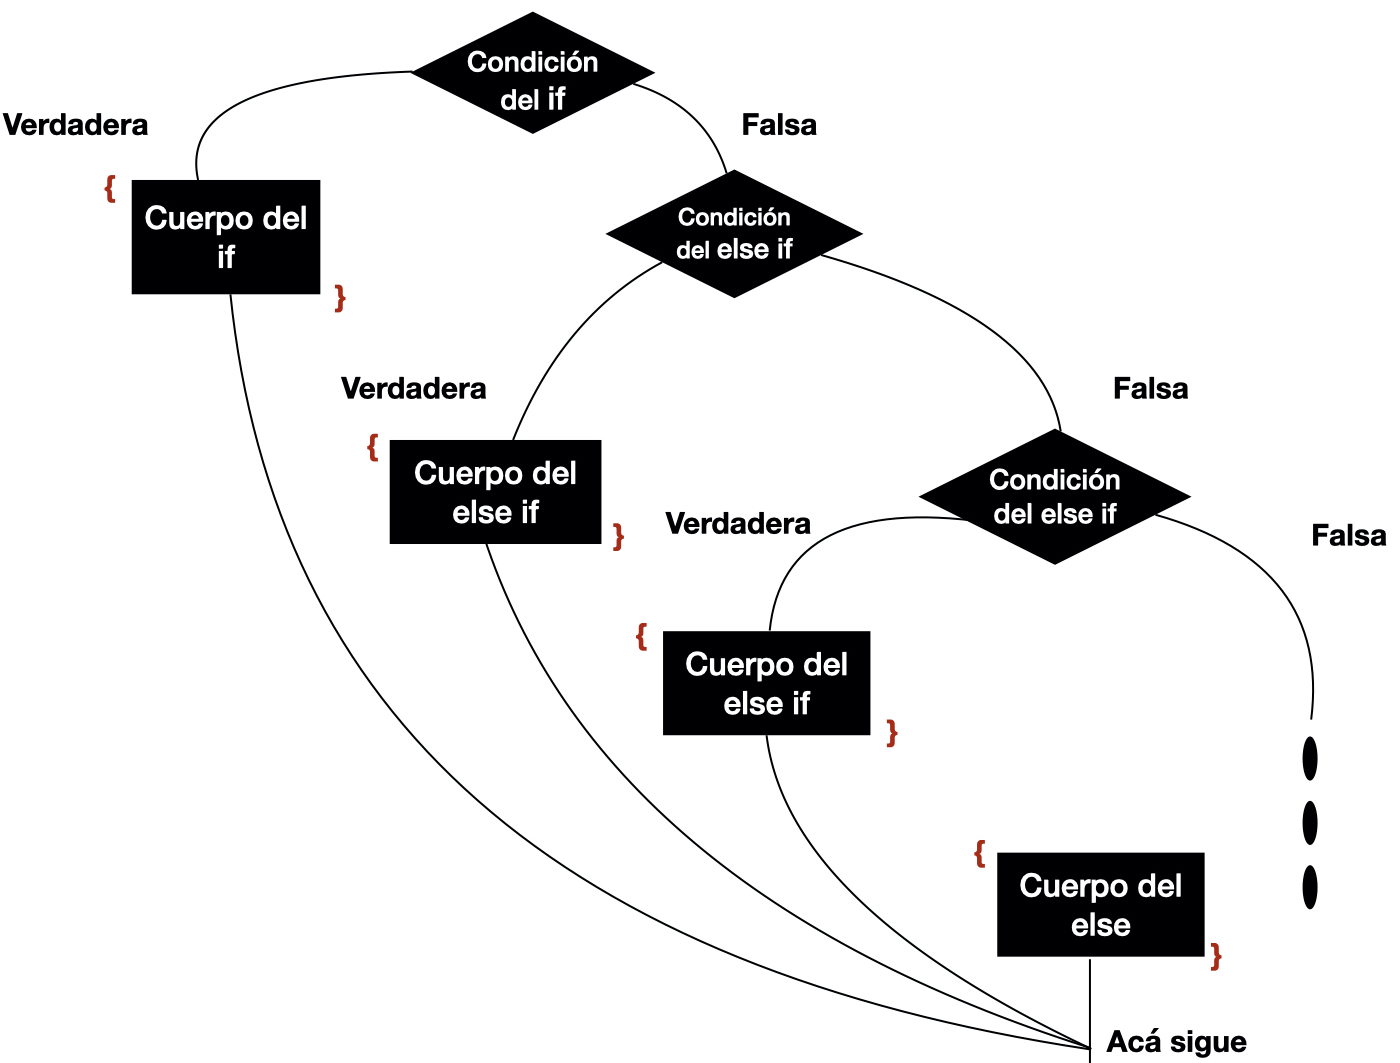
\includegraphics[width=1\textwidth,height=1.5\textheight]{If_else_else_if.001.jpeg}
\caption{Diagrama de flujo del if\ldots{} else if\ldots{} else if\ldots else}\label{id}
}
\end{figure}

\begin{Shaded}
\begin{Highlighting}[]
\NormalTok{numero}\OtherTok{\textless{}{-}}\DecValTok{3}
\ControlFlowTok{if}\NormalTok{(numero }\SpecialCharTok{\textgreater{}} \DecValTok{0}\NormalTok{)\{}
  \FunctionTok{print}\NormalTok{(}\StringTok{"Tu número es positivo"}\NormalTok{)}
\NormalTok{\}}\ControlFlowTok{else} \ControlFlowTok{if}\NormalTok{ (numero }\SpecialCharTok{\textless{}}\DecValTok{0}\NormalTok{)\{}
  \FunctionTok{print}\NormalTok{(}\StringTok{"Tu número es negativo"}\NormalTok{)}
\NormalTok{\}}\ControlFlowTok{else}\NormalTok{\{}
  \FunctionTok{print}\NormalTok{(}\StringTok{"Tu número es cero"}\NormalTok{)}
\NormalTok{\}}
\end{Highlighting}
\end{Shaded}

\begin{verbatim}
## [1] "Tu número es positivo"
\end{verbatim}

\begin{Shaded}
\begin{Highlighting}[]
\NormalTok{numero}\OtherTok{\textless{}{-}} \SpecialCharTok{{-}}\DecValTok{27}
\ControlFlowTok{if}\NormalTok{(numero }\SpecialCharTok{\textgreater{}} \DecValTok{0}\NormalTok{)\{}
  \FunctionTok{print}\NormalTok{(}\StringTok{"Tu número es positivo"}\NormalTok{)}
\NormalTok{\}}\ControlFlowTok{else} \ControlFlowTok{if}\NormalTok{ (numero }\SpecialCharTok{\textless{}}\DecValTok{0}\NormalTok{)\{}
  \FunctionTok{print}\NormalTok{(}\StringTok{"Tu número es negativo"}\NormalTok{)}
\NormalTok{\}}\ControlFlowTok{else}\NormalTok{\{}
  \FunctionTok{print}\NormalTok{(}\StringTok{"Tu número es cero"}\NormalTok{)}
\NormalTok{\}}
\end{Highlighting}
\end{Shaded}

\begin{verbatim}
## [1] "Tu número es negativo"
\end{verbatim}

\begin{Shaded}
\begin{Highlighting}[]
\NormalTok{numero}\OtherTok{\textless{}{-}} \DecValTok{0}
\ControlFlowTok{if}\NormalTok{(numero }\SpecialCharTok{\textgreater{}} \DecValTok{0}\NormalTok{)\{}
  \FunctionTok{print}\NormalTok{(}\StringTok{"Tu número es positivo"}\NormalTok{)}
\NormalTok{\}}\ControlFlowTok{else} \ControlFlowTok{if}\NormalTok{ (numero }\SpecialCharTok{\textless{}}\DecValTok{0}\NormalTok{)\{}
  \FunctionTok{print}\NormalTok{(}\StringTok{"Tu número es negativo"}\NormalTok{)}
\NormalTok{\}}\ControlFlowTok{else}\NormalTok{\{}
  \FunctionTok{print}\NormalTok{(}\StringTok{"Tu número es cero"}\NormalTok{)}
\NormalTok{\}}
\end{Highlighting}
\end{Shaded}

\begin{verbatim}
## [1] "Tu número es cero"
\end{verbatim}

\textbf{Pregunta}: ¿por qué no es necesario poner un if en el último else?

\hypertarget{ejercicios-2}{%
\section{Ejercicios}\label{ejercicios-2}}

\begin{enumerate}
\def\labelenumi{\arabic{enumi}.}
\item
  Elabora un programa que con tu fecha de cumpleaños te diga en qué estación del año naciste.
\item
  Elabora un porgrama que a partir de las calficaciones de tus examenes parciales y 8 quincenales arroje si exentaras o no este curso usando los criterios definidos en el programa del curso. Asume que en las tareas y demás actividades tienes 10.
\end{enumerate}

\begin{center}\rule{0.5\linewidth}{0.5pt}\end{center}

\begin{center}\rule{0.5\linewidth}{0.5pt}\end{center}

\hypertarget{functions}{%
\chapter{Funciones en R}\label{functions}}

Las funciones definidas por el usuario en R son bloques de código que realizan una tarea específica y se pueden llamar desde cualquier lugar del programa. Las funciones en R se definen usando la palabra clave function seguida del nombre de la función, paréntesis y llaves.

Las funciones toman argumentos de entrada y producen un resultado como salida. Las funciones definidas por el usuario son una herramienta poderosa en R que permiten reutilizar código y automatizar tareas. Una vez que domines la sintaxis básica de la función en R, puedes comenzar a crear funciones más avanzadas y complejas para adaptarse a tus necesidades.

\hypertarget{sintaxis-buxe1sica-de-una-funciuxf3n-en-r}{%
\section{Sintaxis básica de una función en R}\label{sintaxis-buxe1sica-de-una-funciuxf3n-en-r}}

La sintaxis básica para definir una función en R es la siguiente:

\begin{Shaded}
\begin{Highlighting}[]
\NormalTok{nombre\_de\_la\_funcion }\OtherTok{\textless{}{-}} \ControlFlowTok{function}\NormalTok{(arg1, arg2, ...) \{}
  \CommentTok{\# Cuerpo de la función}
\NormalTok{  resultado }\OtherTok{\textless{}{-}}\NormalTok{ ...}
  \FunctionTok{return}\NormalTok{(resultado)}
\NormalTok{\}}
\end{Highlighting}
\end{Shaded}

Donde:

\begin{itemize}
\tightlist
\item
  \texttt{nombre\_de\_la\_funcion}: el nombre que le das a tu función. -\texttt{function}: la palabra \emph{function}
\item
  \texttt{arg1}, \texttt{arg2}, \ldots: los argumentos de entrada que toma la función (opcional).
\item
  \texttt{resultado}: el resultado que devuelve la función (opcional).
\end{itemize}

El cuerpo de la función es donde se escribe el código que realiza la tarea específica. El resultado de la función se devuelve con la función \texttt{return()}.

\hypertarget{ejemplo-de-funciuxf3n-definida-por-el-usuario-en-r}{%
\section{Ejemplo de función definida por el usuario en R}\label{ejemplo-de-funciuxf3n-definida-por-el-usuario-en-r}}

Aquí hay un ejemplo de una función definida por el usuario que toma dos argumentos x e y y devuelve la suma de ambos:

\begin{Shaded}
\begin{Highlighting}[]
\NormalTok{mi\_suma }\OtherTok{\textless{}{-}} \ControlFlowTok{function}\NormalTok{(x, y) \{}
\NormalTok{  resultado }\OtherTok{\textless{}{-}}\NormalTok{ x }\SpecialCharTok{+}\NormalTok{ y}
  \FunctionTok{return}\NormalTok{(resultado)}
\NormalTok{\}}
\end{Highlighting}
\end{Shaded}

Para usar esta función, simplemente llámala con los argumentos que deseas pasar:

\begin{Shaded}
\begin{Highlighting}[]
\FunctionTok{mi\_suma}\NormalTok{(}\DecValTok{3}\NormalTok{, }\DecValTok{5}\NormalTok{)}
\end{Highlighting}
\end{Shaded}

\begin{verbatim}
## [1] 8
\end{verbatim}

\hypertarget{ejemplo-de-funciuxf3n-con-argumentos-por-defecto-en-r}{%
\section{Ejemplo de función con argumentos por defecto en R}\label{ejemplo-de-funciuxf3n-con-argumentos-por-defecto-en-r}}

Las funciones en R también pueden tener argumentos por defecto que se utilizan si no se proporciona ningún valor para ellos. Aquí hay un ejemplo de una función que tiene dos argumentos, \texttt{x} e \texttt{y}, y \texttt{y} tiene un valor por defecto de 2:

\begin{Shaded}
\begin{Highlighting}[]
\NormalTok{mi\_funcion }\OtherTok{\textless{}{-}} \ControlFlowTok{function}\NormalTok{(x, }\AttributeTok{y =} \DecValTok{2}\NormalTok{) \{}
\NormalTok{  resultado }\OtherTok{\textless{}{-}}\NormalTok{ x }\SpecialCharTok{*}\NormalTok{ y}
  \FunctionTok{return}\NormalTok{(resultado)}
\NormalTok{\}}
\end{Highlighting}
\end{Shaded}

En este caso, si no se proporciona un valor para \texttt{y}, se utilizará el valor por defecto de \texttt{2}:

\begin{Shaded}
\begin{Highlighting}[]
\FunctionTok{mi\_funcion}\NormalTok{(}\DecValTok{3}\NormalTok{)}
\end{Highlighting}
\end{Shaded}

\begin{verbatim}
## [1] 6
\end{verbatim}

También puede proporcionar un valor diferente para y, si es necesario:

\begin{Shaded}
\begin{Highlighting}[]
\FunctionTok{mi\_funcion}\NormalTok{(}\DecValTok{3}\NormalTok{, }\DecValTok{5}\NormalTok{)}
\end{Highlighting}
\end{Shaded}

\begin{verbatim}
## [1] 15
\end{verbatim}

\hypertarget{definir-una-funciuxf3n-con-un-paruxe1metro-opcional}{%
\section{Definir una función con un parámetro opcional}\label{definir-una-funciuxf3n-con-un-paruxe1metro-opcional}}

\begin{Shaded}
\begin{Highlighting}[]
\NormalTok{saludar }\OtherTok{\textless{}{-}} \ControlFlowTok{function}\NormalTok{(nombre, }\AttributeTok{saludo =} \StringTok{"Hola"}\NormalTok{) \{}
\NormalTok{  mensaje }\OtherTok{\textless{}{-}} \FunctionTok{paste}\NormalTok{(saludo, nombre)}
  \FunctionTok{return}\NormalTok{(mensaje)}
\NormalTok{\}}
\end{Highlighting}
\end{Shaded}

\hypertarget{llamar-a-la-funciuxf3n-saludar-sin-proporcionar-el-paruxe1metro-opcional}{%
\subsection{Llamar a la función saludar sin proporcionar el parámetro opcional}\label{llamar-a-la-funciuxf3n-saludar-sin-proporcionar-el-paruxe1metro-opcional}}

\begin{Shaded}
\begin{Highlighting}[]
\NormalTok{mensaje1 }\OtherTok{\textless{}{-}} \FunctionTok{saludar}\NormalTok{(}\StringTok{"Juan"}\NormalTok{)}
\FunctionTok{print}\NormalTok{(mensaje1)}
\end{Highlighting}
\end{Shaded}

\begin{verbatim}
## [1] "Hola Juan"
\end{verbatim}

\hypertarget{llamar-a-la-funciuxf3n-saludar-proporcionando-el-paruxe1metro-opcional}{%
\subsection{Llamar a la función saludar proporcionando el parámetro opcional}\label{llamar-a-la-funciuxf3n-saludar-proporcionando-el-paruxe1metro-opcional}}

\begin{Shaded}
\begin{Highlighting}[]
\NormalTok{mensaje2 }\OtherTok{\textless{}{-}} \FunctionTok{saludar}\NormalTok{(}\StringTok{"María"}\NormalTok{, }\StringTok{"Buenos días"}\NormalTok{)}
\FunctionTok{print}\NormalTok{(mensaje2)}
\end{Highlighting}
\end{Shaded}

\begin{verbatim}
## [1] "Buenos días María"
\end{verbatim}

\hypertarget{definir-una-funciuxf3n-para-calcular-el-uxe1rea-de-un-cuxedrculo}{%
\section{Definir una función para calcular el área de un círculo}\label{definir-una-funciuxf3n-para-calcular-el-uxe1rea-de-un-cuxedrculo}}

\begin{Shaded}
\begin{Highlighting}[]
\NormalTok{area\_circulo }\OtherTok{\textless{}{-}} \ControlFlowTok{function}\NormalTok{(radio) \{}
\NormalTok{  area }\OtherTok{\textless{}{-}}\NormalTok{ pi }\SpecialCharTok{*}\NormalTok{ radio}\SpecialCharTok{\^{}}\DecValTok{2}
  \FunctionTok{return}\NormalTok{(area)}
\NormalTok{\}}
\CommentTok{\# Ejemplo de uso}

\NormalTok{radio }\OtherTok{\textless{}{-}} \DecValTok{3}
\NormalTok{area }\OtherTok{\textless{}{-}} \FunctionTok{area\_circulo}\NormalTok{(radio)}
\FunctionTok{print}\NormalTok{(}\FunctionTok{paste}\NormalTok{(}\StringTok{"El área del círculo con radio"}\NormalTok{, radio, }\StringTok{"es:"}\NormalTok{, area))}
\end{Highlighting}
\end{Shaded}

\begin{verbatim}
## [1] "El área del círculo con radio 3 es: 28.2743338823081"
\end{verbatim}

\hypertarget{definir-una-funciuxf3n-para-calcular-el-factorial-de-un-nuxfamero}{%
\section{Definir una función para calcular el factorial de un número}\label{definir-una-funciuxf3n-para-calcular-el-factorial-de-un-nuxfamero}}

\begin{Shaded}
\begin{Highlighting}[]
\NormalTok{factorial }\OtherTok{\textless{}{-}} \ControlFlowTok{function}\NormalTok{(n) \{}
  \ControlFlowTok{if}\NormalTok{ (n }\SpecialCharTok{==} \DecValTok{0}\NormalTok{) \{}
    \FunctionTok{return}\NormalTok{(}\DecValTok{1}\NormalTok{)}
\NormalTok{  \} }\ControlFlowTok{else}\NormalTok{ \{}
    \FunctionTok{return}\NormalTok{(n }\SpecialCharTok{*} \FunctionTok{factorial}\NormalTok{(n }\SpecialCharTok{{-}} \DecValTok{1}\NormalTok{))}
\NormalTok{  \}}
\NormalTok{\}}

\CommentTok{\# Ejemplo de uso}
\NormalTok{numero }\OtherTok{\textless{}{-}} \DecValTok{5}
\NormalTok{resultado }\OtherTok{\textless{}{-}} \FunctionTok{factorial}\NormalTok{(numero)}
\FunctionTok{print}\NormalTok{(}\FunctionTok{paste}\NormalTok{(}\StringTok{"El factorial de"}\NormalTok{, numero, }\StringTok{"es:"}\NormalTok{, resultado))}
\end{Highlighting}
\end{Shaded}

\begin{verbatim}
## [1] "El factorial de 5 es: 120"
\end{verbatim}

\hypertarget{definir-una-funciuxf3n-para-verificar-si-un-nuxfamero-es-primo}{%
\section{Definir una función para verificar si un número es primo}\label{definir-una-funciuxf3n-para-verificar-si-un-nuxfamero-es-primo}}

\begin{Shaded}
\begin{Highlighting}[]
\NormalTok{es\_primo }\OtherTok{\textless{}{-}} \ControlFlowTok{function}\NormalTok{(n) \{}
  \ControlFlowTok{if}\NormalTok{ (n }\SpecialCharTok{\textless{}=} \DecValTok{1}\NormalTok{) \{}
    \FunctionTok{return}\NormalTok{(}\ConstantTok{FALSE}\NormalTok{)}
\NormalTok{  \} }\ControlFlowTok{else} \ControlFlowTok{if}\NormalTok{ (n }\SpecialCharTok{\textless{}=} \DecValTok{3}\NormalTok{) \{}
    \FunctionTok{return}\NormalTok{(}\ConstantTok{TRUE}\NormalTok{)}
\NormalTok{  \} }\ControlFlowTok{else} \ControlFlowTok{if}\NormalTok{ (n }\SpecialCharTok{\%\%} \DecValTok{2} \SpecialCharTok{==} \DecValTok{0} \SpecialCharTok{|}\NormalTok{ n }\SpecialCharTok{\%\%} \DecValTok{3} \SpecialCharTok{==} \DecValTok{0}\NormalTok{) \{}
    \FunctionTok{return}\NormalTok{(}\ConstantTok{FALSE}\NormalTok{)}
\NormalTok{  \}}
\NormalTok{  i }\OtherTok{\textless{}{-}} \DecValTok{5}
  \ControlFlowTok{while}\NormalTok{ (i }\SpecialCharTok{*}\NormalTok{ i }\SpecialCharTok{\textless{}=}\NormalTok{ n) \{}
    \ControlFlowTok{if}\NormalTok{ (n }\SpecialCharTok{\%\%}\NormalTok{ i }\SpecialCharTok{==} \DecValTok{0} \SpecialCharTok{|}\NormalTok{ n }\SpecialCharTok{\%\%}\NormalTok{ (i }\SpecialCharTok{+} \DecValTok{2}\NormalTok{) }\SpecialCharTok{==} \DecValTok{0}\NormalTok{) \{}
      \FunctionTok{return}\NormalTok{(}\ConstantTok{FALSE}\NormalTok{)}
\NormalTok{    \}}
\NormalTok{    i }\OtherTok{\textless{}{-}}\NormalTok{ i }\SpecialCharTok{+} \DecValTok{6}
\NormalTok{  \}}
  \FunctionTok{return}\NormalTok{(}\ConstantTok{TRUE}\NormalTok{)}
\NormalTok{\}}

\CommentTok{\# Ejemplo de uso}
\NormalTok{numero }\OtherTok{\textless{}{-}} \DecValTok{11}
\ControlFlowTok{if}\NormalTok{ (}\FunctionTok{es\_primo}\NormalTok{(numero)) \{}
  \FunctionTok{print}\NormalTok{(}\FunctionTok{paste}\NormalTok{(numero, }\StringTok{"es un número primo."}\NormalTok{))}
\NormalTok{\} }\ControlFlowTok{else}\NormalTok{ \{}
  \FunctionTok{print}\NormalTok{(}\FunctionTok{paste}\NormalTok{(numero, }\StringTok{"no es un número primo."}\NormalTok{))}
\NormalTok{\}}
\end{Highlighting}
\end{Shaded}

\begin{verbatim}
## [1] "11 es un número primo."
\end{verbatim}

\textbf{Ejercicios}

\begin{enumerate}
\def\labelenumi{\arabic{enumi}.}
\item
  Escribe una función que tome un vector numérico como argumento de entrada y devuelva la media aritmética de los valores.
\item
  Escribe una función que tome dos vectores numéricos como argumentos de entrada y devuelva su producto punto (también conocido como producto escalar).
\item
  Escribe una función que tome un vector numérico como argumento de entrada y devuelva el valor mínimo y máximo en una lista.
\item
  Escribe una función que tome una matriz cuadrada como argumento de entrada y devuelva su determinante.
\item
  Escribe una función que tome una matriz de \(2 \times 2\) como argumento de entrada y devuelva su transpuesta.
\item
  Escribe una función que tome una lista como argumento de entrada y devuelva la longitud de cada elemento en una lista.
\item
  Escribe una función que tome una cadena de texto como argumento de entrada y devuelva una lista con todas las palabras en la cadena.
\item
  Escribe una función que tome un vector numérico como argumento de entrada y devuelva un vector con los valores ordenados de menor a mayor.
\item
  Escribe una función que tome un vector de caracteres como argumento de entrada y devuelva un vector con los mismos elementos en orden inverso.
\item
  Escribe una función que tome una matriz como argumento de entrada y devuelva la diagonal principal en un vector.
\end{enumerate}

\hypertarget{rprojects}{%
\chapter{RProjects}\label{rprojects}}

Los proyectos en R (R Projects) son una manera eficiente de organizar y gestionar todo el trabajo relacionado con tus análisis en R. Facilitan la colaboración, el control de versiones y la reproducibilidad de tu investigación o análisis de datos.

\hypertarget{introducciuxf3n-a-r-projects-en-rstudio}{%
\section{Introducción a R Projects en RStudio}\label{introducciuxf3n-a-r-projects-en-rstudio}}

RStudio permite crear proyectos, que son básicamente carpetas que contienen todos los archivos relacionados con un análisis específico. Al trabajar dentro de un proyecto, RStudio automáticamente establece el directorio del proyecto como el directorio de trabajo, simplificando la gestión de archivos y el flujo de trabajo.

\textbf{Crear un nuevo proyecto:}

\begin{enumerate}
\def\labelenumi{\arabic{enumi}.}
\tightlist
\item
  En RStudio, ve a \texttt{File\ \textgreater{}\ New\ Project}.
\item
  Elige crear un proyecto en un nuevo directorio o en un directorio existente.
\item
  Asigna un nombre al proyecto y selecciona la ubicación para el directorio del proyecto.
\item
  Haz clic en \texttt{Create\ Project}.
\end{enumerate}

\hypertarget{gestiuxf3n-de-proyectos-organizaciuxf3n-y-buenas-pruxe1cticas}{%
\section{Gestión de proyectos: organización y buenas prácticas}\label{gestiuxf3n-de-proyectos-organizaciuxf3n-y-buenas-pruxe1cticas}}

Una buena gestión de proyectos en R implica una estructura de carpetas organizada, nomenclatura consistente de archivos y un entendimiento claro del flujo de trabajo del proyecto.

\textbf{Estructura de carpetas recomendada:}

\begin{itemize}
\tightlist
\item
  \texttt{/01\_RawData}: Guarda tus bases de datos originales (preferentemente en formato de solo lectura como .csv o .xlsx)..
\item
  \texttt{/02\_Scripts}: Guardar tus scripts con extensiones .R o .Rmd
\item
  \texttt{/03\_ProceesedData}: Almacena archivos de salida procesados, como datos limpios o tablas resumen
\item
  \texttt{/04\_output}: .Guarda las figuras generadas por tus scripts.
\end{itemize}

\textbf{Buenas prácticas:}

\begin{itemize}
\tightlist
\item
  Mantén un script de R (por ejemplo, \texttt{main.R}) que sirva como punto de entrada para entender y ejecutar el proyecto.
\item
  Documenta tus scripts detalladamente para que otros (o tú en el futuro) puedan entender el propósito y funcionamiento de tu código.
\item
  Utiliza nombres de archivos y variables claros y descriptivos.
\end{itemize}

\hypertarget{colaboraciuxf3n-y-control-de-versiones-con-git-y-github}{%
\section{Colaboración y control de versiones con Git y GitHub}\label{colaboraciuxf3n-y-control-de-versiones-con-git-y-github}}

El control de versiones es crucial para la colaboración en proyectos de programación. Git, integrado con GitHub, permite a múltiples personas trabajar en el mismo proyecto sin conflictos.

\textbf{Configurar Git en RStudio:}

\begin{enumerate}
\def\labelenumi{\arabic{enumi}.}
\tightlist
\item
  Instala Git en tu computadora y configúralo con tus credenciales de GitHub.
\item
  En RStudio, ve a \texttt{Tools\ \textgreater{}\ Global\ Options\ \textgreater{}\ Git/SVN} para configurar tu cuenta de Git.
\item
  Crea un nuevo repositorio en GitHub y clónalo en tu computadora a través de la URL del repositorio.
\end{enumerate}

\textbf{Uso básico de Git con RStudio:}

\begin{itemize}
\tightlist
\item
  \textbf{Commit}: Guarda los cambios realizados en tus archivos al repositorio local. Describe brevemente los cambios realizados.
\item
  \textbf{Push}: Envía tus commits locales a GitHub para actualizar el repositorio remoto.
\item
  \textbf{Pull}: Actualiza tu repositorio local con los cambios realizados por otros colaboradores en el repositorio remoto.
\end{itemize}

\textbf{Colaborar en proyectos:}

\begin{itemize}
\tightlist
\item
  Utiliza \emph{branches} para trabajar en nuevas características o experimentos sin afectar la rama principal (\emph{main} o \emph{master}).
\item
  Abre \emph{pull requests} para discutir cambios antes de integrarlos a la rama principal.
\item
  Realiza revisiones de código y utiliza \emph{issues} para rastrear tareas y discutir problemas.
\end{itemize}

\hypertarget{visualizaciuxf3n-de-datos-con-ggplot2}{%
\chapter{Visualización de datos con ggplot2}\label{visualizaciuxf3n-de-datos-con-ggplot2}}

\hypertarget{introducciuxf3n}{%
\section{Introducción}\label{introducciuxf3n}}

La visualización de datos es una herramienta poderosa en el análisis de datos, permitiendo comunicar información compleja de manera intuitiva y efectiva. \texttt{ggplot2} es un paquete en R que facilita la creación de gráficos de calidad de publicación de manera sencilla. Este documento proporciona una introducción a \texttt{ggplot2} y ejercicios para practicar.

\hypertarget{configuraciuxf3n-inicial}{%
\section{Configuración inicial}\label{configuraciuxf3n-inicial}}

Primero, asegúrate de tener instalado \texttt{ggplot2}.

\begin{Shaded}
\begin{Highlighting}[]
\FunctionTok{library}\NormalTok{(ggplot2)}
\end{Highlighting}
\end{Shaded}

\hypertarget{creaciuxf3n-de-un-gruxe1fico-buxe1sico}{%
\section{Creación de un gráfico básico}\label{creaciuxf3n-de-un-gruxe1fico-buxe1sico}}

Vamos a comenzar con un gráfico de dispersión simple utilizando el conjunto de datos mtcars.

\begin{Shaded}
\begin{Highlighting}[]
\FunctionTok{ggplot}\NormalTok{(}\AttributeTok{data =}\NormalTok{ mtcars, }\FunctionTok{aes}\NormalTok{(}\AttributeTok{x =}\NormalTok{ wt, }\AttributeTok{y =}\NormalTok{ mpg)) }\SpecialCharTok{+} 
  \FunctionTok{geom\_point}\NormalTok{() }\SpecialCharTok{+}
  \FunctionTok{labs}\NormalTok{(}\AttributeTok{title =} \StringTok{"Consumo de Gasolina vs. Peso"}\NormalTok{,}
       \AttributeTok{x =} \StringTok{"Peso (1000 lbs)"}\NormalTok{,}
       \AttributeTok{y =} \StringTok{"Millas por Galón (mpg)"}\NormalTok{)}
\end{Highlighting}
\end{Shaded}

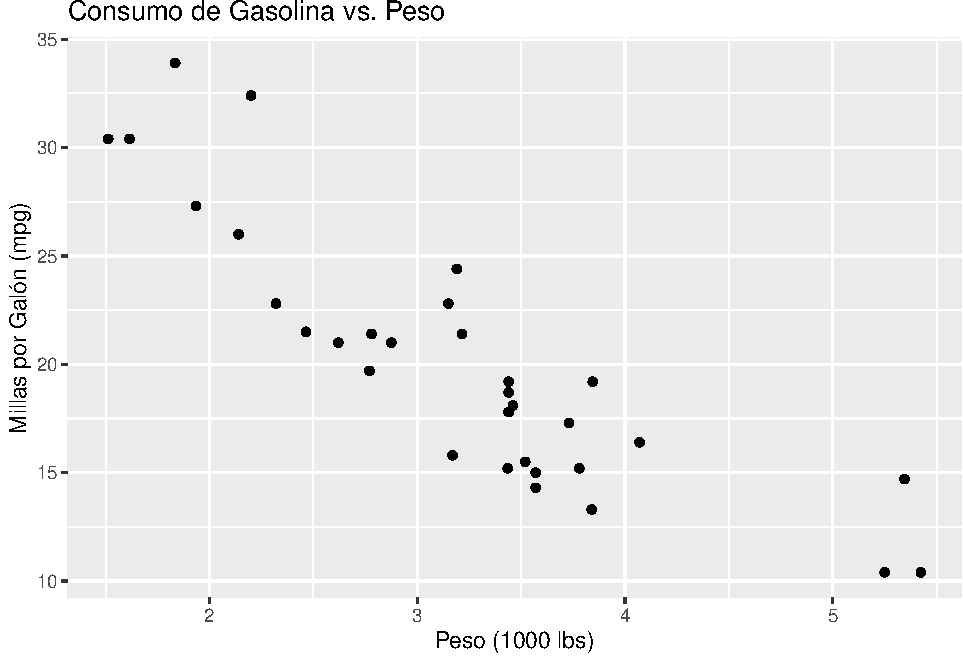
\includegraphics{bookdown-demo_files/figure-latex/unnamed-chunk-170-1.pdf}

\hypertarget{personalizaciuxf3n-de-gruxe1ficos}{%
\section{Personalización de gráficos}\label{personalizaciuxf3n-de-gruxe1ficos}}

Ahora, personalizaremos el gráfico cambiando colores y añadiendo una línea de tendencia.

\begin{Shaded}
\begin{Highlighting}[]
\FunctionTok{ggplot}\NormalTok{(}\AttributeTok{data =}\NormalTok{ mtcars, }\FunctionTok{aes}\NormalTok{(}\AttributeTok{x =}\NormalTok{ wt, }\AttributeTok{y =}\NormalTok{ mpg, }\AttributeTok{color =} \FunctionTok{factor}\NormalTok{(gear))) }\SpecialCharTok{+} 
  \FunctionTok{geom\_point}\NormalTok{() }\SpecialCharTok{+}
  \FunctionTok{geom\_smooth}\NormalTok{(}\AttributeTok{method =} \StringTok{"lm"}\NormalTok{, }\AttributeTok{se =} \ConstantTok{FALSE}\NormalTok{) }\SpecialCharTok{+}
  \FunctionTok{labs}\NormalTok{(}\AttributeTok{title =} \StringTok{"Consumo de Gasolina vs. Peso por Tipo de Cambio"}\NormalTok{,}
       \AttributeTok{x =} \StringTok{"Peso (1000 lbs)"}\NormalTok{,}
       \AttributeTok{y =} \StringTok{"Millas por Galón (mpg)"}\NormalTok{,}
       \AttributeTok{color =} \StringTok{"Tipo de Cambio"}\NormalTok{) }\SpecialCharTok{+}
  \FunctionTok{theme\_minimal}\NormalTok{()}
\end{Highlighting}
\end{Shaded}

\begin{verbatim}
## `geom_smooth()` using formula = 'y ~ x'
\end{verbatim}

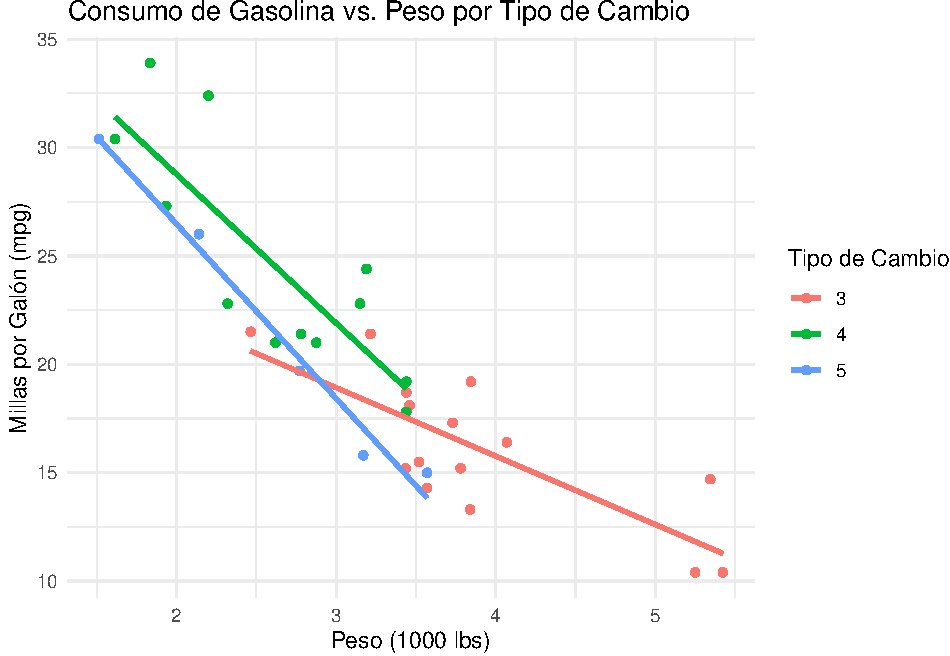
\includegraphics{bookdown-demo_files/figure-latex/unnamed-chunk-171-1.pdf}
\#\#\# Ejercicios sugeridos

\begin{enumerate}
\def\labelenumi{\arabic{enumi}.}
\tightlist
\item
  Explora otro conjunto de datos: Utiliza el conjunto de datos iris para crear un gráfico de dispersión que muestre la relación entre Sepal.Length y Sepal.Width. Colorea los puntos según la especie.
\item
  Personaliza tu gráfico: Añade títulos personalizados a los ejes y al gráfico. Experimenta con diferentes temas, como theme\_bw() o theme\_light().
\item
  Exploración de geométricas: Utiliza geom\_histogram() para crear un histograma del Sepal.Length en el conjunto de datos iris. Ajusta los parámetros binwidth y fill.
\item
  Facetas para múltiples gráficos: Utiliza facet\_wrap(\textasciitilde{} species) para crear gráficos separados para cada especie en el conjunto de datos iris, mostrando la relación entre Sepal.Length y Sepal.Width.
\end{enumerate}

\hypertarget{soluciones-a-los-ejercicios-sugeridos}{%
\section{Soluciones a los ejercicios sugeridos}\label{soluciones-a-los-ejercicios-sugeridos}}

\begin{Shaded}
\begin{Highlighting}[]
\FunctionTok{ggplot}\NormalTok{(}\AttributeTok{data =}\NormalTok{ iris, }\FunctionTok{aes}\NormalTok{(}\AttributeTok{x =}\NormalTok{ Sepal.Length, }\AttributeTok{y =}\NormalTok{ Sepal.Width, }\AttributeTok{color =}\NormalTok{ Species)) }\SpecialCharTok{+} 
  \FunctionTok{geom\_point}\NormalTok{() }\SpecialCharTok{+}
  \FunctionTok{labs}\NormalTok{(}\AttributeTok{title =} \StringTok{"Relación entre el Largo y el Ancho del Sépalo por Especie"}\NormalTok{,}
       \AttributeTok{x =} \StringTok{"Largo del Sépalo"}\NormalTok{,}
       \AttributeTok{y =} \StringTok{"Ancho del Sépalo"}\NormalTok{)}
\end{Highlighting}
\end{Shaded}

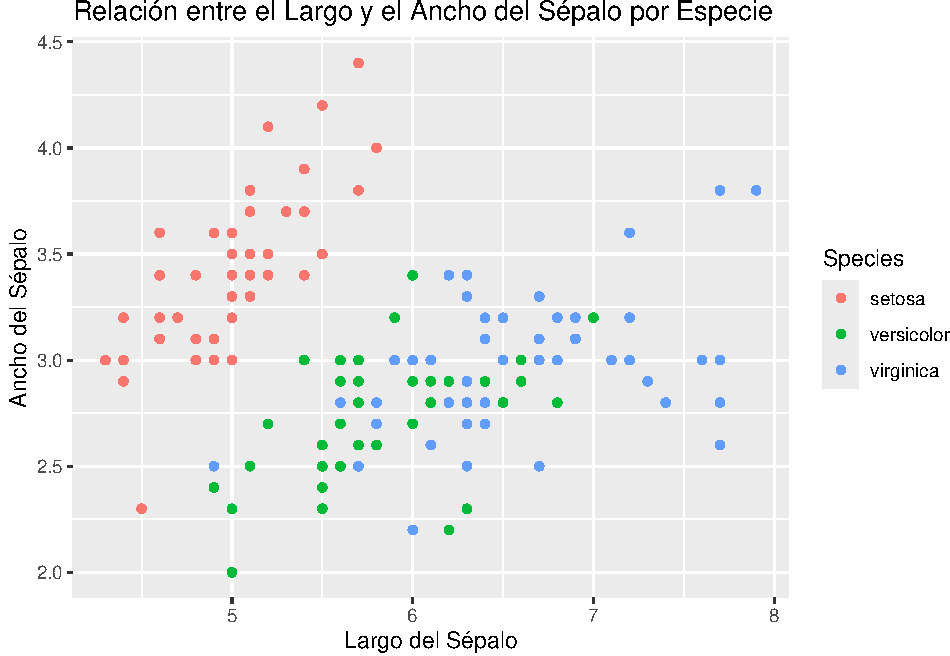
\includegraphics{bookdown-demo_files/figure-latex/unnamed-chunk-172-1.pdf}

\begin{Shaded}
\begin{Highlighting}[]
\FunctionTok{ggplot}\NormalTok{(}\AttributeTok{data =}\NormalTok{ iris, }\FunctionTok{aes}\NormalTok{(}\AttributeTok{x =}\NormalTok{ Sepal.Length, }\AttributeTok{y =}\NormalTok{ Sepal.Width, }\AttributeTok{color =}\NormalTok{ Species)) }\SpecialCharTok{+} 
  \FunctionTok{geom\_point}\NormalTok{() }\SpecialCharTok{+}
  \FunctionTok{labs}\NormalTok{(}\AttributeTok{title =} \StringTok{"Relación entre el Largo y el Ancho del Sépalo por Especie"}\NormalTok{,}
       \AttributeTok{x =} \StringTok{"Largo del Sépalo"}\NormalTok{,}
       \AttributeTok{y =} \StringTok{"Ancho del Sépalo"}\NormalTok{) }\SpecialCharTok{+}
  \FunctionTok{theme\_light}\NormalTok{() }\SpecialCharTok{+}
  \FunctionTok{theme}\NormalTok{(}\AttributeTok{legend.title =} \FunctionTok{element\_blank}\NormalTok{())}
\end{Highlighting}
\end{Shaded}

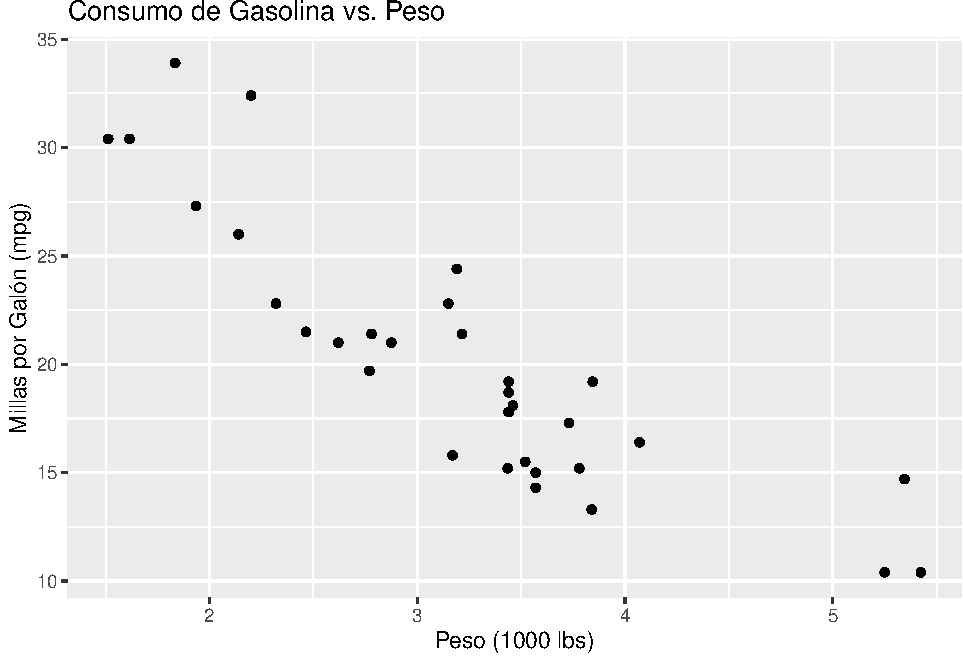
\includegraphics{bookdown-demo_files/figure-latex/unnamed-chunk-173-1.pdf}

\begin{Shaded}
\begin{Highlighting}[]
\FunctionTok{ggplot}\NormalTok{(}\AttributeTok{data =}\NormalTok{ iris, }\FunctionTok{aes}\NormalTok{(}\AttributeTok{x =}\NormalTok{ Sepal.Length)) }\SpecialCharTok{+} 
  \FunctionTok{geom\_histogram}\NormalTok{(}\AttributeTok{binwidth =} \FloatTok{0.5}\NormalTok{, }\AttributeTok{fill =} \StringTok{"blue"}\NormalTok{) }\SpecialCharTok{+}
  \FunctionTok{labs}\NormalTok{(}\AttributeTok{title =} \StringTok{"Distribución del Largo del Sépalo"}\NormalTok{,}
       \AttributeTok{x =} \StringTok{"Largo del Sépalo"}\NormalTok{,}
       \AttributeTok{y =} \StringTok{"Frecuencia"}\NormalTok{)}
\end{Highlighting}
\end{Shaded}

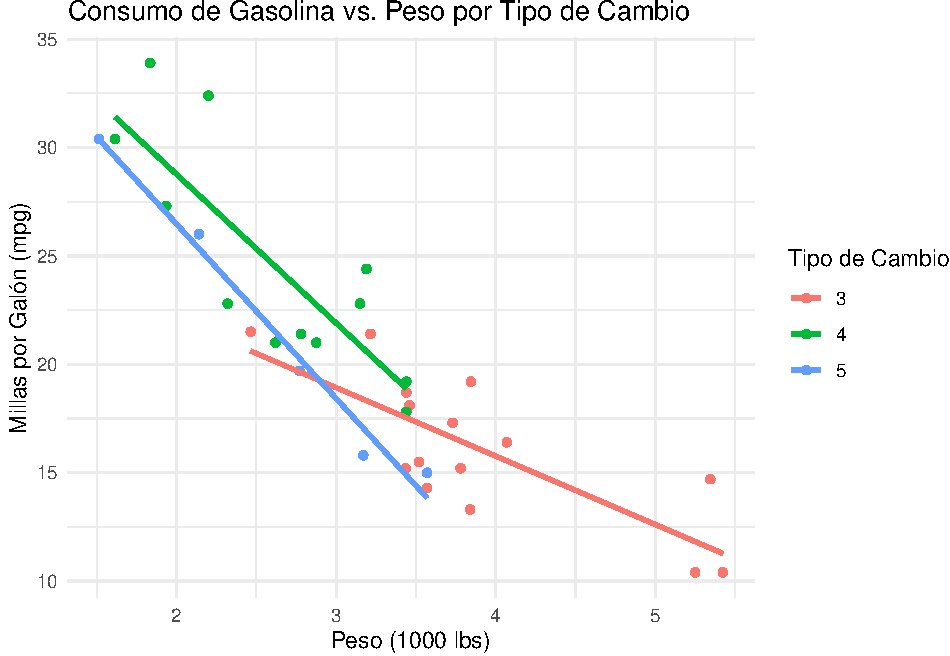
\includegraphics{bookdown-demo_files/figure-latex/unnamed-chunk-174-1.pdf}

\begin{Shaded}
\begin{Highlighting}[]
\FunctionTok{ggplot}\NormalTok{(}\AttributeTok{data =}\NormalTok{ iris, }\FunctionTok{aes}\NormalTok{(}\AttributeTok{x =}\NormalTok{ Sepal.Length, }\AttributeTok{y =}\NormalTok{ Sepal.Width)) }\SpecialCharTok{+} 
  \FunctionTok{geom\_point}\NormalTok{() }\SpecialCharTok{+}
  \FunctionTok{facet\_wrap}\NormalTok{(}\SpecialCharTok{\textasciitilde{}}\NormalTok{ Species) }\SpecialCharTok{+}
  \FunctionTok{labs}\NormalTok{(}\AttributeTok{title =} \StringTok{"Relación entre el Largo y el Ancho del Sépalo por Especie"}\NormalTok{,}
       \AttributeTok{x =} \StringTok{"Largo del Sépalo"}\NormalTok{,}
       \AttributeTok{y =} \StringTok{"Ancho del Sépalo"}\NormalTok{)}
\end{Highlighting}
\end{Shaded}

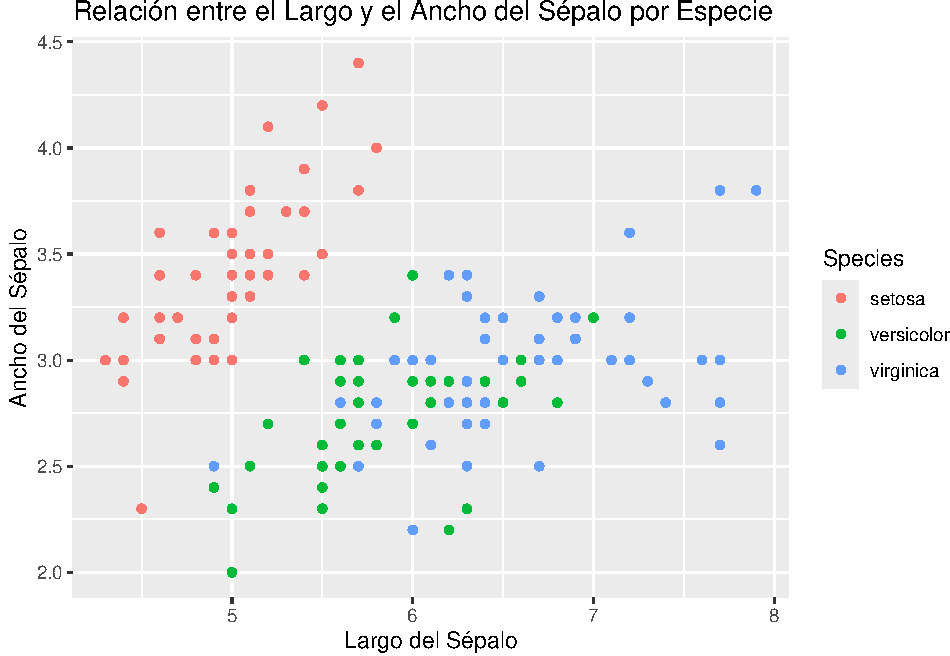
\includegraphics{bookdown-demo_files/figure-latex/unnamed-chunk-175-1.pdf}

\hypertarget{ejercicios-resueltos}{%
\section{Ejercicios resueltos}\label{ejercicios-resueltos}}

En esta sección usaremos la librería \texttt{palmerpenguins}

\begin{Shaded}
\begin{Highlighting}[]
\FunctionTok{library}\NormalTok{(palmerpenguins)}
\FunctionTok{library}\NormalTok{(ggplot2)}
\end{Highlighting}
\end{Shaded}

\hypertarget{ejercicio-1-gruxe1fico-de-dispersiuxf3n-buxe1sico}{%
\subsection{Ejercicio 1: Gráfico de dispersión básico}\label{ejercicio-1-gruxe1fico-de-dispersiuxf3n-buxe1sico}}

Crea un gráfico de dispersión para visualizar la relación entre la longitud del culmen y la profundidad del culmen de los pingüinos.

\begin{Shaded}
\begin{Highlighting}[]
\FunctionTok{ggplot}\NormalTok{(penguins, }\FunctionTok{aes}\NormalTok{(}\AttributeTok{x =}\NormalTok{ bill\_length\_mm, }\AttributeTok{y =}\NormalTok{ bill\_depth\_mm)) }\SpecialCharTok{+}
  \FunctionTok{geom\_point}\NormalTok{()}
\end{Highlighting}
\end{Shaded}

\begin{verbatim}
## Warning: Removed 2 rows containing missing values or values outside the scale range
## (`geom_point()`).
\end{verbatim}

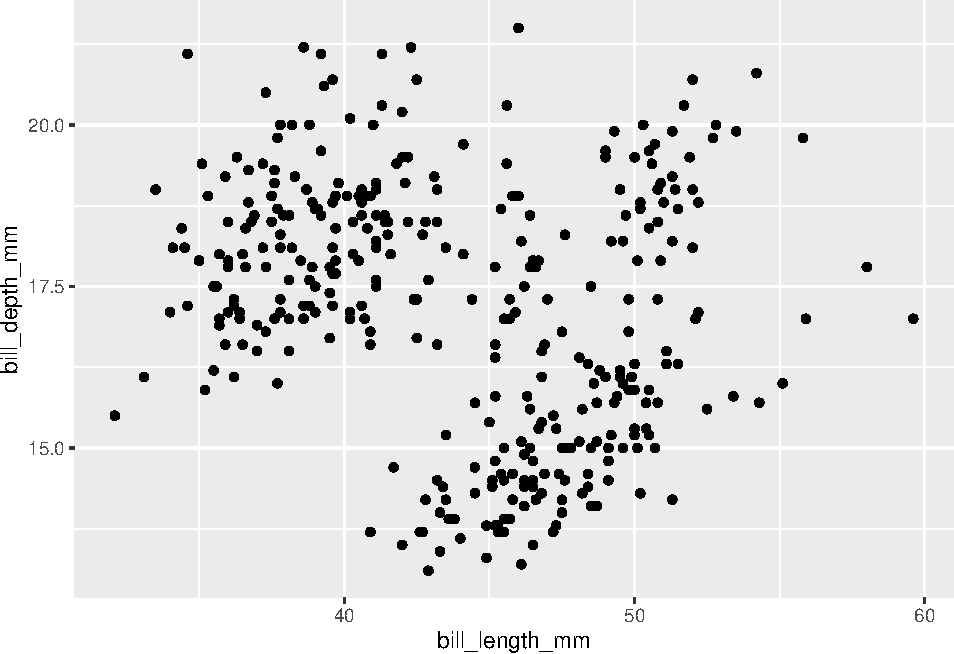
\includegraphics{bookdown-demo_files/figure-latex/unnamed-chunk-177-1.pdf}

\hypertarget{ejercicio-2-diferenciaciuxf3n-por-especie}{%
\subsection{Ejercicio 2: Diferenciación por especie}\label{ejercicio-2-diferenciaciuxf3n-por-especie}}

Modifica el gráfico de dispersión anterior para diferenciar los puntos por especie de pingüino.

\begin{Shaded}
\begin{Highlighting}[]
\FunctionTok{ggplot}\NormalTok{(penguins, }\FunctionTok{aes}\NormalTok{(}\AttributeTok{x =}\NormalTok{ bill\_length\_mm, }\AttributeTok{y =}\NormalTok{ bill\_depth\_mm, }\AttributeTok{color =}\NormalTok{ species)) }\SpecialCharTok{+}
  \FunctionTok{geom\_point}\NormalTok{()}
\end{Highlighting}
\end{Shaded}

\begin{verbatim}
## Warning: Removed 2 rows containing missing values or values outside the scale range
## (`geom_point()`).
\end{verbatim}

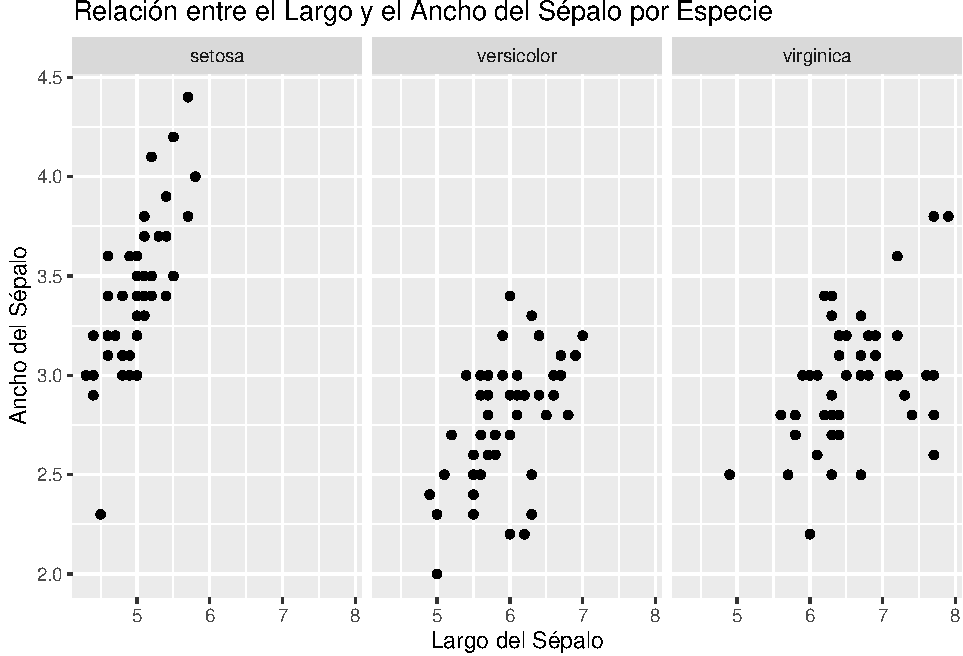
\includegraphics{bookdown-demo_files/figure-latex/unnamed-chunk-178-1.pdf}

\hypertarget{ejercicio-3-histograma-de-masa-corporal}{%
\subsection{Ejercicio 3: Histograma de masa corporal}\label{ejercicio-3-histograma-de-masa-corporal}}

Crea un histograma para explorar la distribución de la masa corporal de los pingüinos.

\begin{Shaded}
\begin{Highlighting}[]
\FunctionTok{ggplot}\NormalTok{(penguins, }\FunctionTok{aes}\NormalTok{(}\AttributeTok{x =}\NormalTok{ body\_mass\_g)) }\SpecialCharTok{+}
  \FunctionTok{geom\_histogram}\NormalTok{(}\AttributeTok{bins =} \DecValTok{30}\NormalTok{)}
\end{Highlighting}
\end{Shaded}

\begin{verbatim}
## Warning: Removed 2 rows containing non-finite outside the scale range
## (`stat_bin()`).
\end{verbatim}

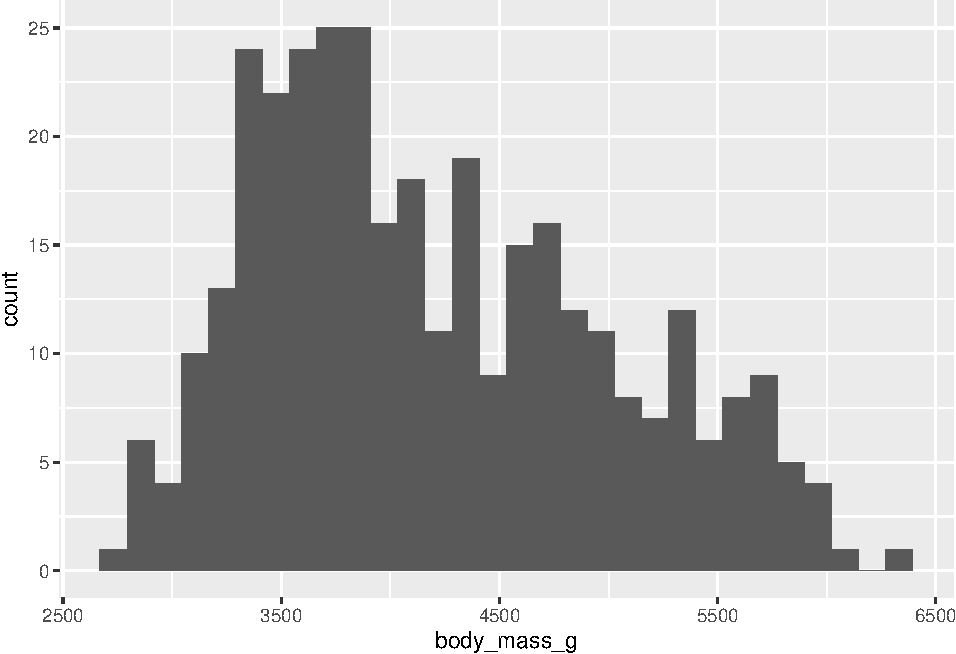
\includegraphics{bookdown-demo_files/figure-latex/unnamed-chunk-179-1.pdf}

\hypertarget{ejercicio-4-barras-de-error-por-especie}{%
\subsection{Ejercicio 4: Barras de error por especie}\label{ejercicio-4-barras-de-error-por-especie}}

Genera un gráfico de barras que muestre la masa corporal media de los pingüinos por especie, incluyendo barras de error.

\begin{Shaded}
\begin{Highlighting}[]
\FunctionTok{ggplot}\NormalTok{(penguins, }\FunctionTok{aes}\NormalTok{(}\AttributeTok{x =}\NormalTok{ species, }\AttributeTok{y =}\NormalTok{ body\_mass\_g)) }\SpecialCharTok{+}
  \FunctionTok{geom\_bar}\NormalTok{(}\AttributeTok{stat =} \StringTok{"summary"}\NormalTok{, }\AttributeTok{fun =} \StringTok{"mean"}\NormalTok{) }\SpecialCharTok{+}
  \FunctionTok{geom\_errorbar}\NormalTok{(}\AttributeTok{stat =} \StringTok{"summary"}\NormalTok{, }\AttributeTok{fun.data =}\NormalTok{ mean\_se, }\AttributeTok{width =} \FloatTok{0.2}\NormalTok{)}
\end{Highlighting}
\end{Shaded}

\begin{verbatim}
## Warning: Removed 2 rows containing non-finite outside the scale range
## (`stat_summary()`).
## Removed 2 rows containing non-finite outside the scale range
## (`stat_summary()`).
\end{verbatim}

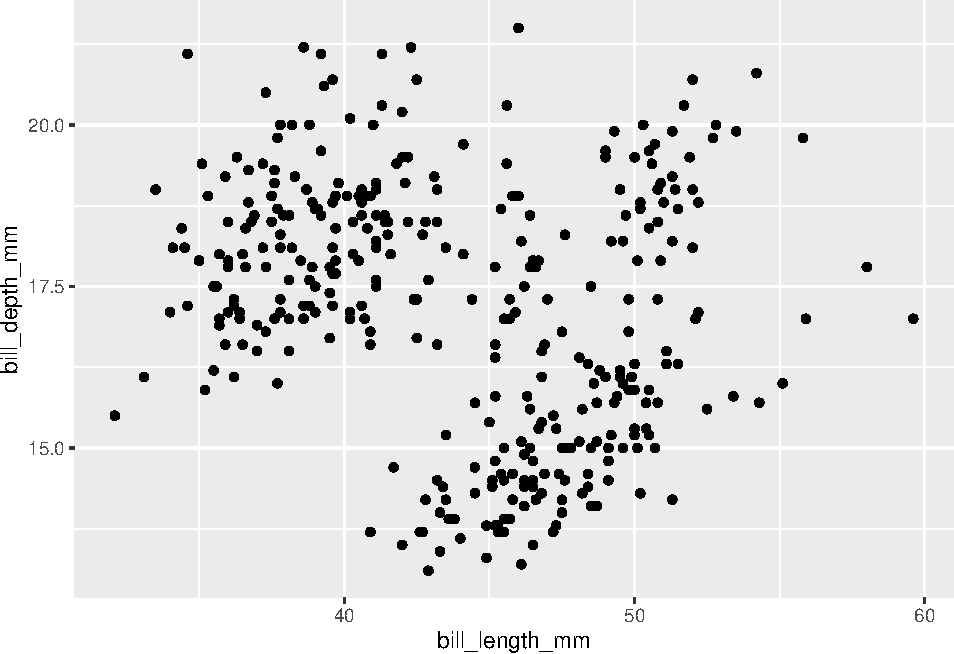
\includegraphics{bookdown-demo_files/figure-latex/unnamed-chunk-180-1.pdf}

\#\#\#Ejercicio 5: Boxplot de profundidad del culmen
Crea un boxplot para comparar la profundidad del culmen entre las diferentes especies de pingüinos.

\begin{Shaded}
\begin{Highlighting}[]
\FunctionTok{ggplot}\NormalTok{(penguins, }\FunctionTok{aes}\NormalTok{(}\AttributeTok{x =}\NormalTok{ species, }\AttributeTok{y =}\NormalTok{ bill\_depth\_mm)) }\SpecialCharTok{+}
  \FunctionTok{geom\_boxplot}\NormalTok{()}
\end{Highlighting}
\end{Shaded}

\begin{verbatim}
## Warning: Removed 2 rows containing non-finite outside the scale range
## (`stat_boxplot()`).
\end{verbatim}

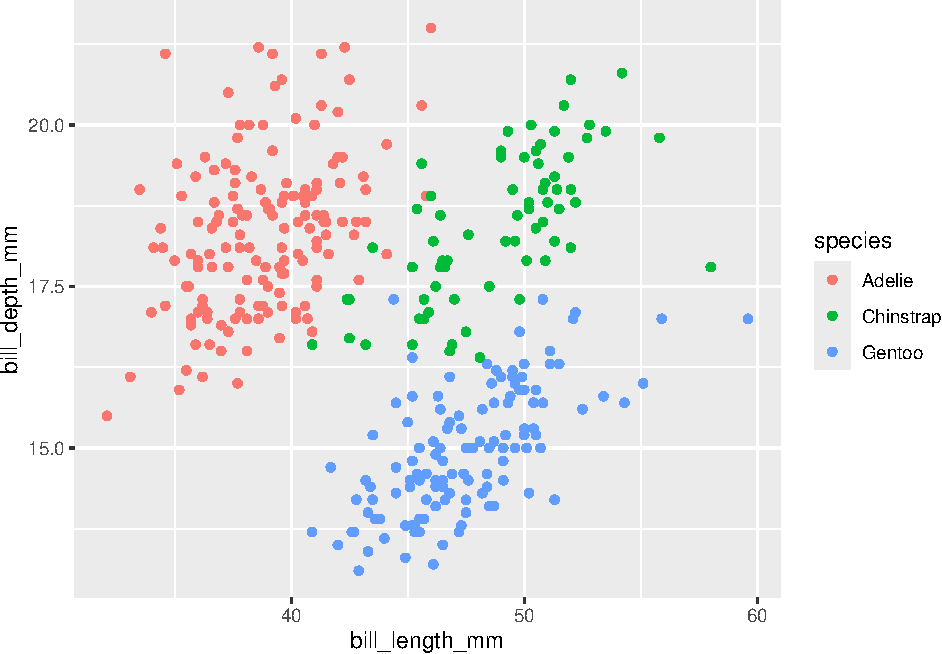
\includegraphics{bookdown-demo_files/figure-latex/unnamed-chunk-181-1.pdf}

\hypertarget{ejercicio-6-facetado-por-islas}{%
\subsection{Ejercicio 6: Facetado por islas}\label{ejercicio-6-facetado-por-islas}}

Repite el gráfico de dispersión de longitud vs.~profundidad del culmen, pero esta vez facetado por la isla de origen.

\begin{Shaded}
\begin{Highlighting}[]
\FunctionTok{ggplot}\NormalTok{(penguins, }\FunctionTok{aes}\NormalTok{(}\AttributeTok{x =}\NormalTok{ bill\_length\_mm, }\AttributeTok{y =}\NormalTok{ bill\_depth\_mm)) }\SpecialCharTok{+}
  \FunctionTok{geom\_point}\NormalTok{() }\SpecialCharTok{+}
  \FunctionTok{facet\_wrap}\NormalTok{(}\SpecialCharTok{\textasciitilde{}}\NormalTok{island)}
\end{Highlighting}
\end{Shaded}

\begin{verbatim}
## Warning: Removed 2 rows containing missing values or values outside the scale range
## (`geom_point()`).
\end{verbatim}

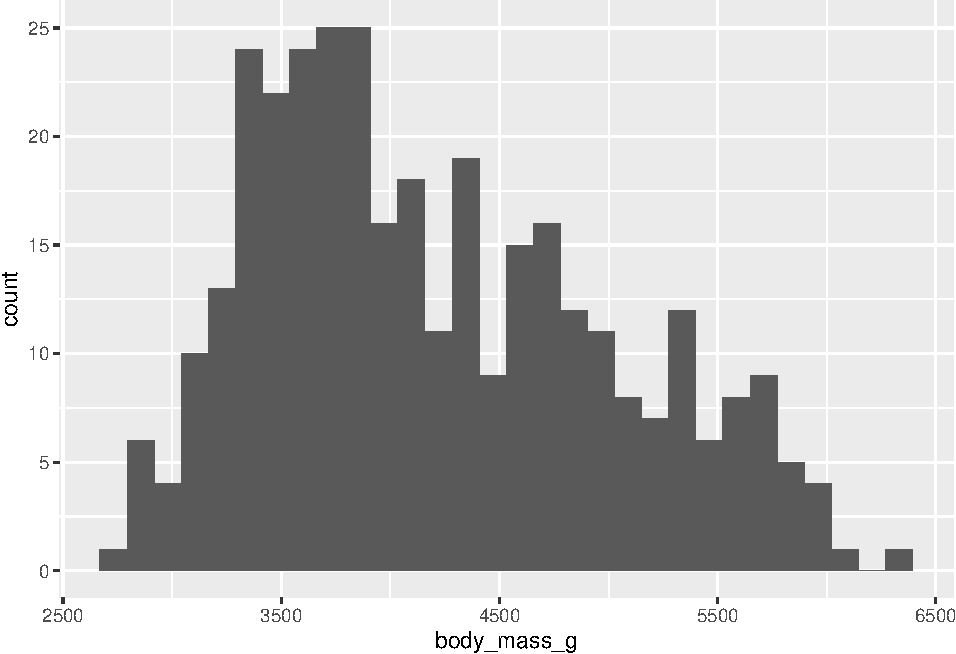
\includegraphics{bookdown-demo_files/figure-latex/unnamed-chunk-182-1.pdf}

\hypertarget{ejercicio-7-densidad-de-masa-corporal}{%
\subsection{Ejercicio 7: Densidad de masa corporal}\label{ejercicio-7-densidad-de-masa-corporal}}

Muestra la densidad de la distribución de la masa corporal de los pingüinos utilizando un gráfico de densidad.

\begin{Shaded}
\begin{Highlighting}[]
\FunctionTok{ggplot}\NormalTok{(penguins, }\FunctionTok{aes}\NormalTok{(}\AttributeTok{x =}\NormalTok{ body\_mass\_g, }\AttributeTok{fill =}\NormalTok{ species)) }\SpecialCharTok{+}
  \FunctionTok{geom\_density}\NormalTok{(}\AttributeTok{alpha =} \FloatTok{0.7}\NormalTok{)}
\end{Highlighting}
\end{Shaded}

\begin{verbatim}
## Warning: Removed 2 rows containing non-finite outside the scale range
## (`stat_density()`).
\end{verbatim}

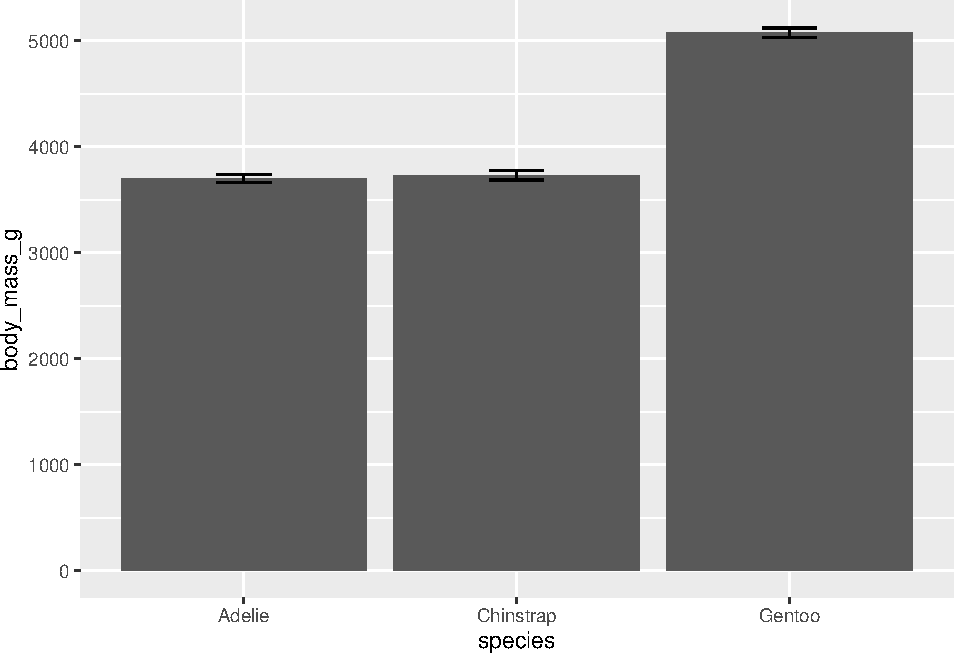
\includegraphics{bookdown-demo_files/figure-latex/unnamed-chunk-183-1.pdf}

\hypertarget{ejercicio-8-gruxe1fico-de-violuxedn-de-la-longitud-del-culmen}{%
\subsection{Ejercicio 8: Gráfico de violín de la longitud del culmen}\label{ejercicio-8-gruxe1fico-de-violuxedn-de-la-longitud-del-culmen}}

Genera un gráfico de violín para visualizar la distribución de la longitud del culmen por especie.

\begin{Shaded}
\begin{Highlighting}[]
\FunctionTok{ggplot}\NormalTok{(penguins, }\FunctionTok{aes}\NormalTok{(}\AttributeTok{x =}\NormalTok{ species, }\AttributeTok{y =}\NormalTok{ bill\_length\_mm)) }\SpecialCharTok{+}
  \FunctionTok{geom\_violin}\NormalTok{()}
\end{Highlighting}
\end{Shaded}

\begin{verbatim}
## Warning: Removed 2 rows containing non-finite outside the scale range
## (`stat_ydensity()`).
\end{verbatim}

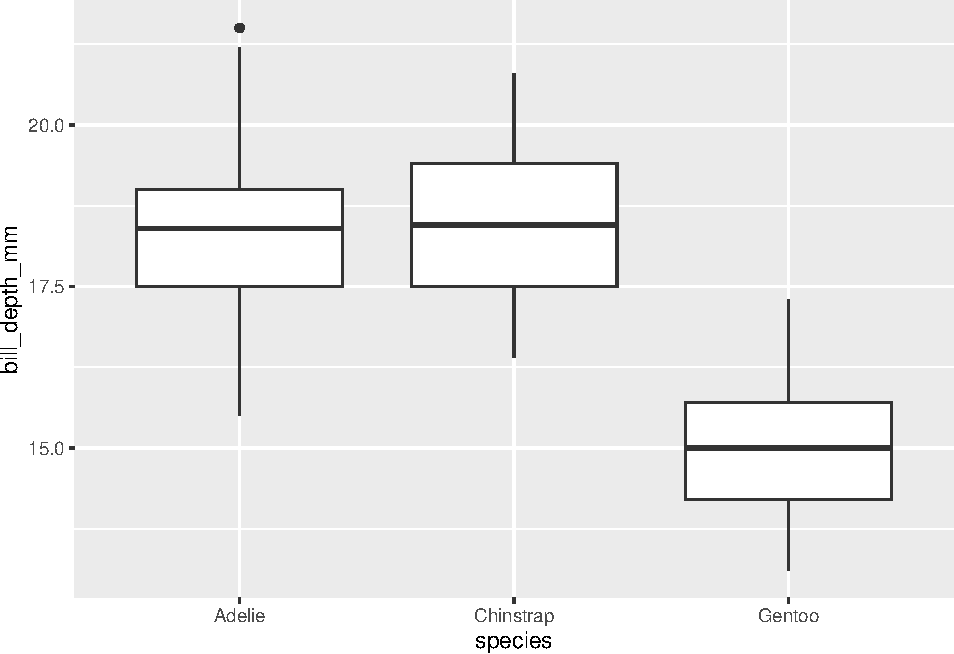
\includegraphics{bookdown-demo_files/figure-latex/unnamed-chunk-184-1.pdf}

\hypertarget{ejercicio-9-puntos-superpuestos-en-boxplot}{%
\subsection{Ejercicio 9: Puntos superpuestos en boxplot}\label{ejercicio-9-puntos-superpuestos-en-boxplot}}

Crea un boxplot de la profundidad del culmen por especie y superpón los puntos de datos individuales.

\begin{Shaded}
\begin{Highlighting}[]
\FunctionTok{ggplot}\NormalTok{(penguins, }\FunctionTok{aes}\NormalTok{(}\AttributeTok{x =}\NormalTok{ species, }\AttributeTok{y =}\NormalTok{ bill\_depth\_mm)) }\SpecialCharTok{+}
  \FunctionTok{geom\_boxplot}\NormalTok{(}\AttributeTok{alpha =} \FloatTok{0.5}\NormalTok{) }\SpecialCharTok{+}
  \FunctionTok{geom\_jitter}\NormalTok{(}\AttributeTok{width =} \FloatTok{0.2}\NormalTok{)}
\end{Highlighting}
\end{Shaded}

\begin{verbatim}
## Warning: Removed 2 rows containing non-finite outside the scale range
## (`stat_boxplot()`).
\end{verbatim}

\begin{verbatim}
## Warning: Removed 2 rows containing missing values or values outside the scale range
## (`geom_point()`).
\end{verbatim}

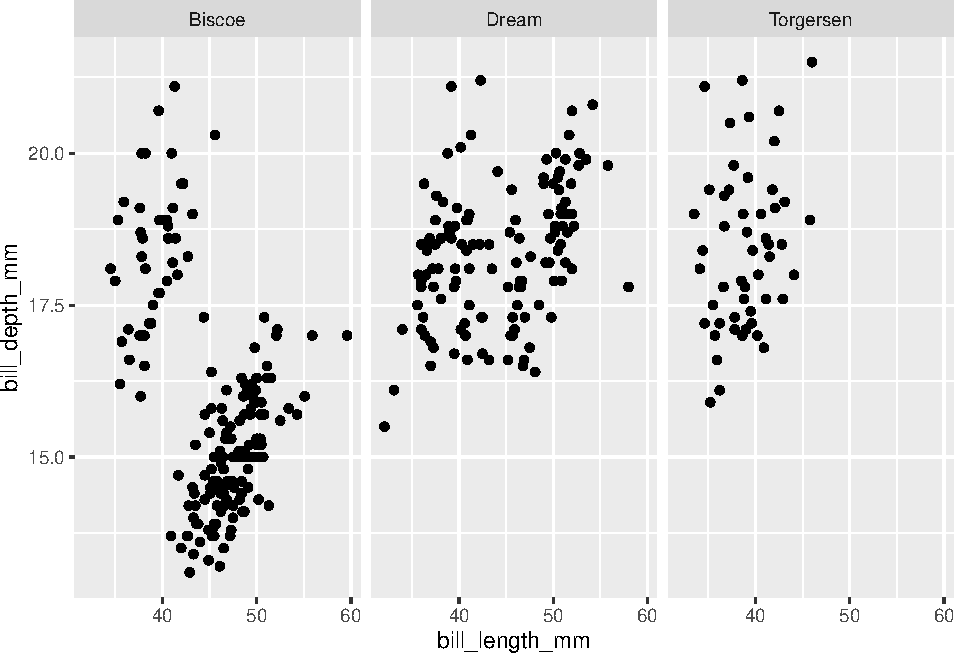
\includegraphics{bookdown-demo_files/figure-latex/unnamed-chunk-185-1.pdf}

\hypertarget{ejercicio-10-gruxe1fico-de-luxedneas-de-masa-corporal-promedio-a-lo-largo-del-tiempo}{%
\subsection{Ejercicio 10: Gráfico de líneas de masa corporal promedio a lo largo del tiempo}\label{ejercicio-10-gruxe1fico-de-luxedneas-de-masa-corporal-promedio-a-lo-largo-del-tiempo}}

Asumiendo que los datos estén ordenados temporalmente, muestra cómo cambia la masa corporal promedio a lo largo del tiempo.

\begin{Shaded}
\begin{Highlighting}[]
\CommentTok{\# Asumiendo que \textquotesingle{}year\textquotesingle{} representa el tiempo en tus datos}
\FunctionTok{ggplot}\NormalTok{(penguins, }\FunctionTok{aes}\NormalTok{(}\AttributeTok{x =}\NormalTok{ year, }\AttributeTok{y =}\NormalTok{ body\_mass\_g, }\AttributeTok{group =} \DecValTok{1}\NormalTok{)) }\SpecialCharTok{+}
  \FunctionTok{geom\_line}\NormalTok{(}\AttributeTok{stat =} \StringTok{"summary"}\NormalTok{, }\AttributeTok{fun =} \StringTok{"mean"}\NormalTok{)}
\end{Highlighting}
\end{Shaded}

\begin{verbatim}
## Warning: Removed 2 rows containing non-finite outside the scale range
## (`stat_summary()`).
\end{verbatim}

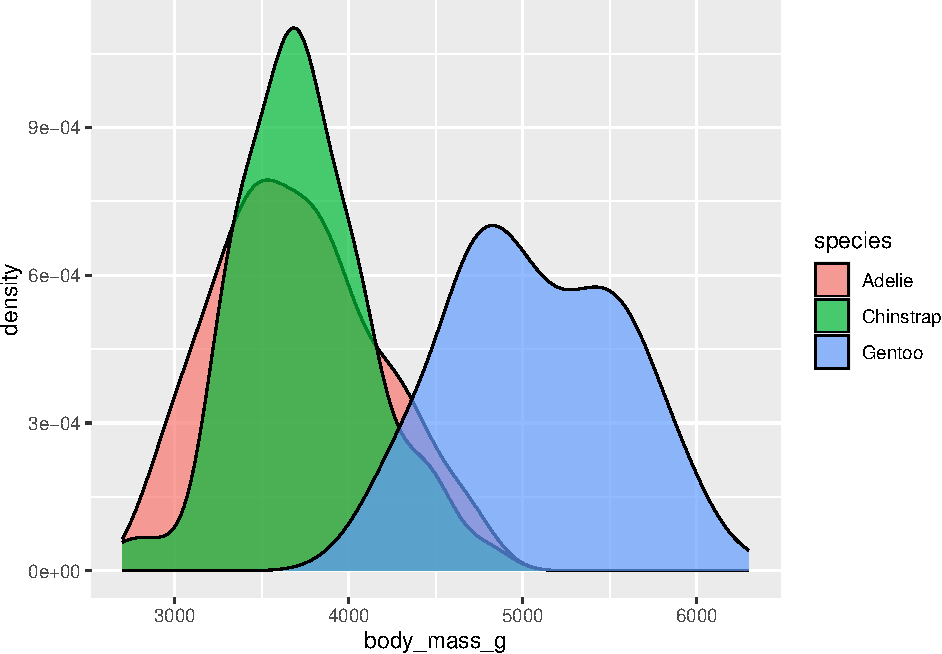
\includegraphics{bookdown-demo_files/figure-latex/unnamed-chunk-186-1.pdf}

\hypertarget{ejercicio-11-gruxe1fico-de-dispersiuxf3n-con-tamauxf1o-de-punto}{%
\subsection{Ejercicio 11: Gráfico de dispersión con tamaño de punto}\label{ejercicio-11-gruxe1fico-de-dispersiuxf3n-con-tamauxf1o-de-punto}}

Modifica el gráfico de dispersión de longitud vs.~profundidad del culmen para que el tamaño de los puntos refleje la masa corporal de los pingüinos.

\begin{Shaded}
\begin{Highlighting}[]
\FunctionTok{ggplot}\NormalTok{(penguins, }\FunctionTok{aes}\NormalTok{(}\AttributeTok{x =}\NormalTok{ bill\_length\_mm, }\AttributeTok{y =}\NormalTok{ bill\_depth\_mm, }\AttributeTok{size =}\NormalTok{ body\_mass\_g)) }\SpecialCharTok{+}
  \FunctionTok{geom\_point}\NormalTok{(}\AttributeTok{alpha =} \FloatTok{0.5}\NormalTok{)}
\end{Highlighting}
\end{Shaded}

\begin{verbatim}
## Warning: Removed 2 rows containing missing values or values outside the scale range
## (`geom_point()`).
\end{verbatim}

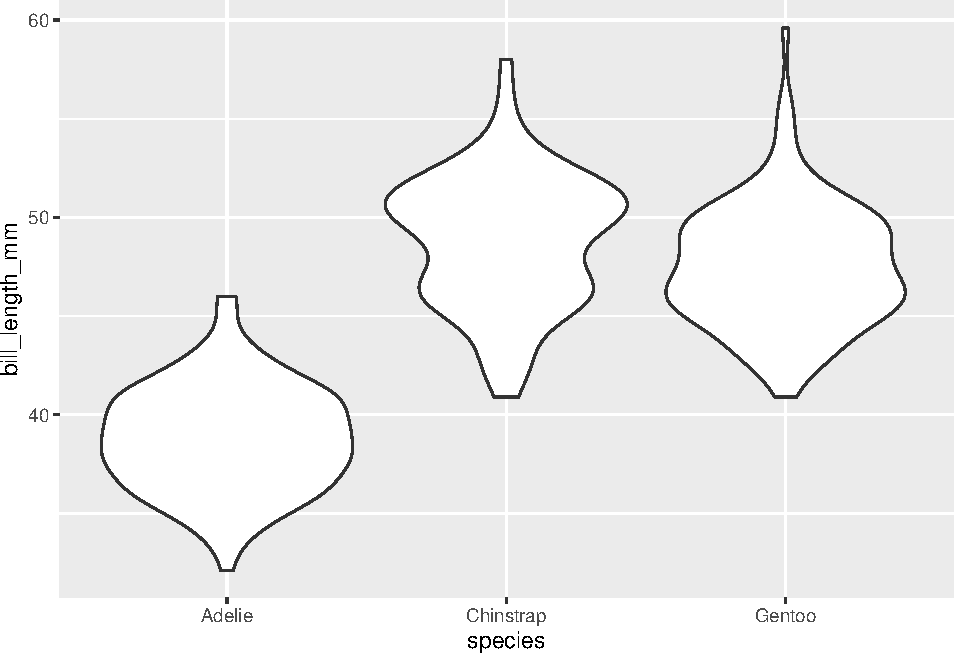
\includegraphics{bookdown-demo_files/figure-latex/unnamed-chunk-187-1.pdf}

\hypertarget{ejercicio-12-barras-apiladas-de-especies-por-isla}{%
\subsection{Ejercicio 12: Barras apiladas de especies por isla}\label{ejercicio-12-barras-apiladas-de-especies-por-isla}}

Crea un gráfico de barras apiladas que muestre la cantidad de pingüinos de cada especie presentes en cada isla.

\begin{Shaded}
\begin{Highlighting}[]
\FunctionTok{ggplot}\NormalTok{(penguins, }\FunctionTok{aes}\NormalTok{(}\AttributeTok{x =}\NormalTok{ island, }\AttributeTok{fill =}\NormalTok{ species)) }\SpecialCharTok{+}
  \FunctionTok{geom\_bar}\NormalTok{(}\AttributeTok{position =} \StringTok{"stack"}\NormalTok{)}
\end{Highlighting}
\end{Shaded}

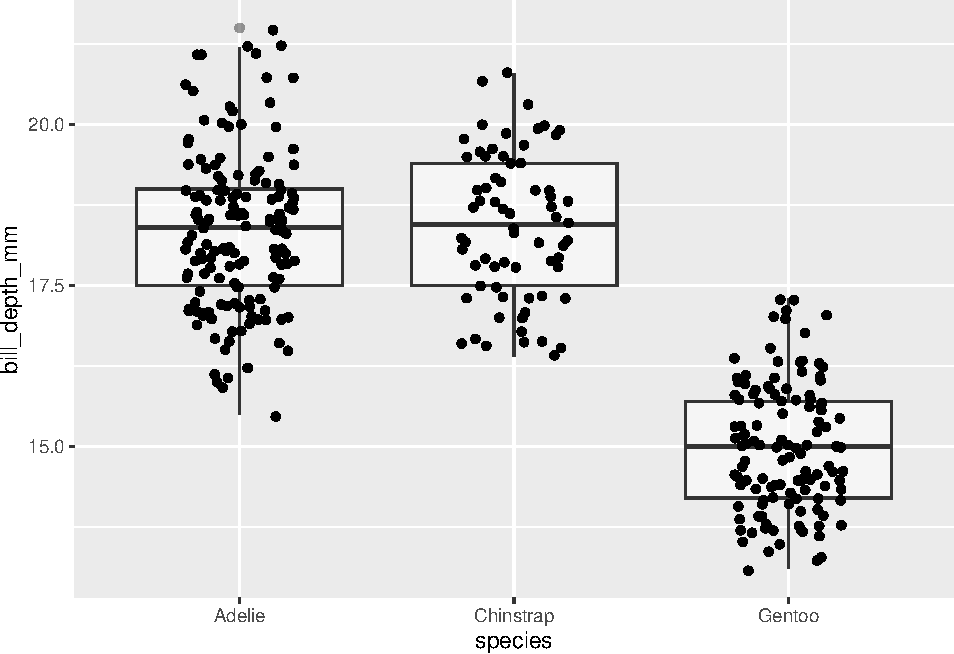
\includegraphics{bookdown-demo_files/figure-latex/unnamed-chunk-188-1.pdf}

\hypertarget{ejercicio-13-gruxe1fico-de-correlaciuxf3n-con-texto}{%
\subsection{Ejercicio 13: Gráfico de correlación con texto}\label{ejercicio-13-gruxe1fico-de-correlaciuxf3n-con-texto}}

Genera un gráfico de dispersión entre la longitud y la profundidad del culmen e incluye un texto que muestre el coeficiente de correlación en el gráfico.

\begin{Shaded}
\begin{Highlighting}[]
\FunctionTok{library}\NormalTok{(ggpubr)}
\FunctionTok{ggplot}\NormalTok{(penguins, }\FunctionTok{aes}\NormalTok{(}\AttributeTok{x =}\NormalTok{ bill\_length\_mm, }\AttributeTok{y =}\NormalTok{ bill\_depth\_mm)) }\SpecialCharTok{+}
  \FunctionTok{geom\_point}\NormalTok{() }\SpecialCharTok{+}
  \FunctionTok{stat\_cor}\NormalTok{(}\AttributeTok{method =} \StringTok{"pearson"}\NormalTok{, }\AttributeTok{label.x =} \DecValTok{3}\NormalTok{, }\AttributeTok{label.y =} \DecValTok{50}\NormalTok{)}
\end{Highlighting}
\end{Shaded}

\begin{verbatim}
## Warning: Removed 2 rows containing non-finite outside the scale range
## (`stat_cor()`).
\end{verbatim}

\begin{verbatim}
## Warning: Removed 2 rows containing missing values or values outside the scale range
## (`geom_point()`).
\end{verbatim}

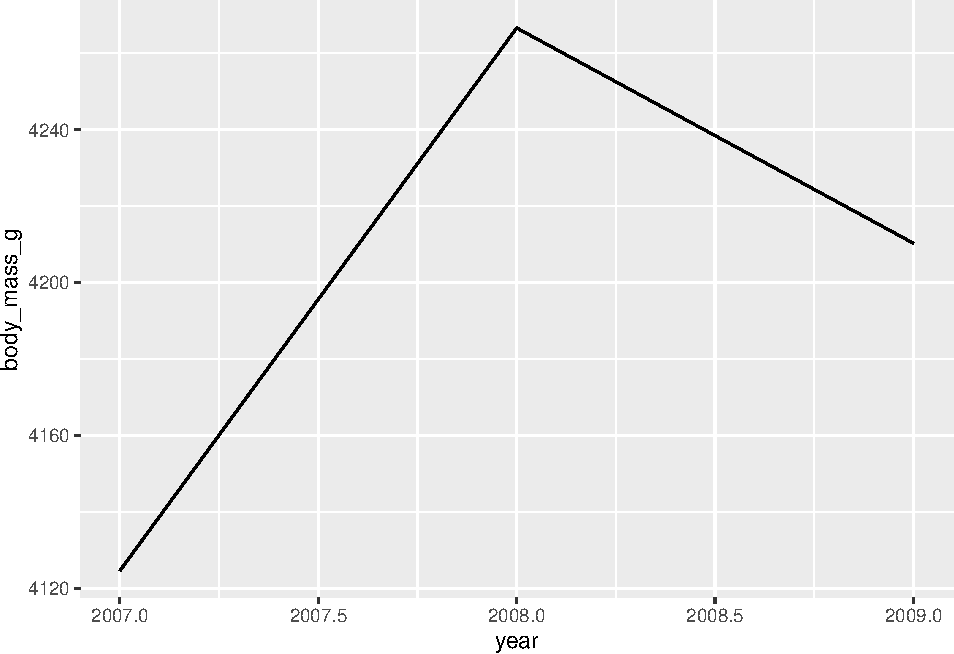
\includegraphics{bookdown-demo_files/figure-latex/unnamed-chunk-189-1.pdf}

\hypertarget{ejercicio-14-mapa-de-calor-de-la-longitud-y-profundidad-del-culmen}{%
\subsection{Ejercicio 14: Mapa de calor de la longitud y profundidad del culmen}\label{ejercicio-14-mapa-de-calor-de-la-longitud-y-profundidad-del-culmen}}

Crea un mapa de calor que muestre la distribución conjunta de la longitud y la profundidad del culmen de los pingüinos.

\begin{Shaded}
\begin{Highlighting}[]
\FunctionTok{ggplot}\NormalTok{(penguins, }\FunctionTok{aes}\NormalTok{(}\AttributeTok{x =}\NormalTok{ bill\_length\_mm, }\AttributeTok{y =}\NormalTok{ bill\_depth\_mm)) }\SpecialCharTok{+}
  \FunctionTok{geom\_bin2d}\NormalTok{()}
\end{Highlighting}
\end{Shaded}

\begin{verbatim}
## Warning: Removed 2 rows containing non-finite outside the scale range
## (`stat_bin2d()`).
\end{verbatim}

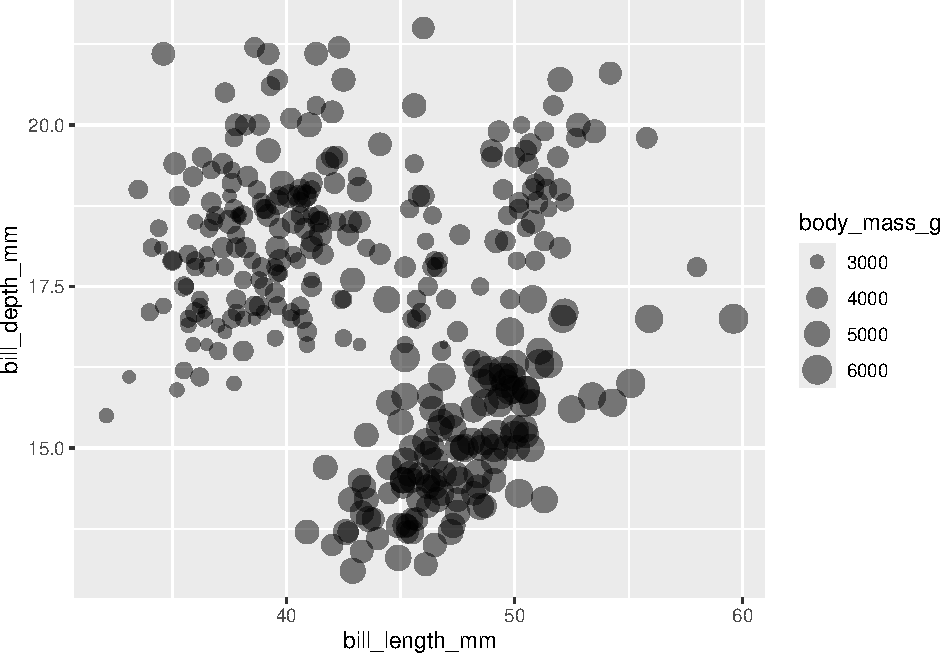
\includegraphics{bookdown-demo_files/figure-latex/unnamed-chunk-190-1.pdf}

\hypertarget{ejercicio-15-gruxe1fico-de-interacciuxf3n-entre-tres-variables}{%
\subsection{Ejercicio 15: Gráfico de interacción entre tres variables}\label{ejercicio-15-gruxe1fico-de-interacciuxf3n-entre-tres-variables}}

Explora la relación entre la longitud del culmen, la profundidad del culmen y la masa corporal, diferenciando por especie.

\begin{Shaded}
\begin{Highlighting}[]
\FunctionTok{ggplot}\NormalTok{(penguins, }\FunctionTok{aes}\NormalTok{(}\AttributeTok{x =}\NormalTok{ bill\_length\_mm, }\AttributeTok{y =}\NormalTok{ bill\_depth\_mm, }\AttributeTok{color =}\NormalTok{ body\_mass\_g)) }\SpecialCharTok{+}
  \FunctionTok{geom\_point}\NormalTok{() }\SpecialCharTok{+}
  \FunctionTok{facet\_wrap}\NormalTok{(}\SpecialCharTok{\textasciitilde{}}\NormalTok{species)}
\end{Highlighting}
\end{Shaded}

\begin{verbatim}
## Warning: Removed 2 rows containing missing values or values outside the scale range
## (`geom_point()`).
\end{verbatim}

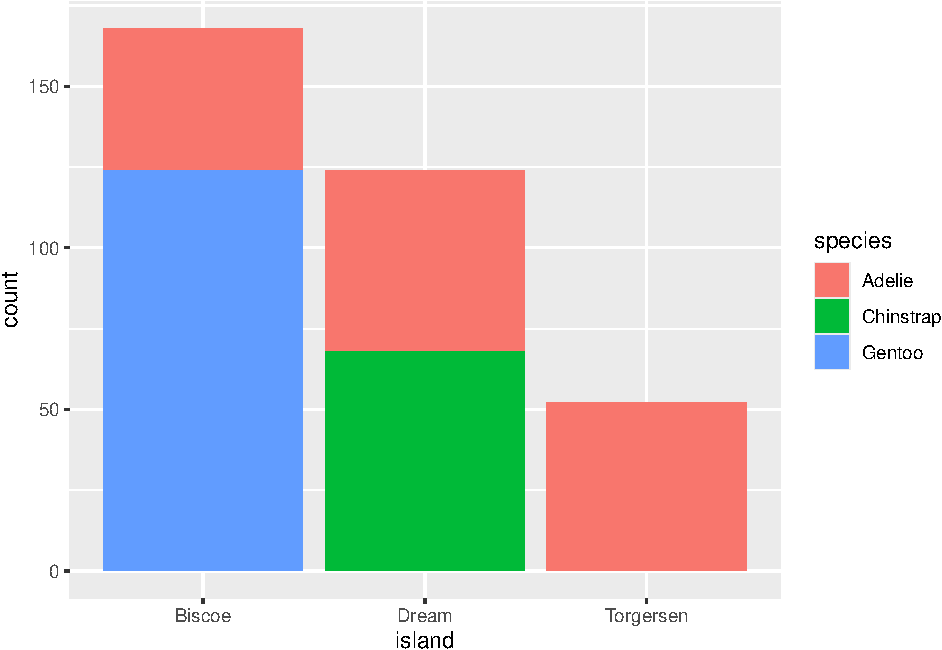
\includegraphics{bookdown-demo_files/figure-latex/unnamed-chunk-191-1.pdf}

\hypertarget{ejercicios-propuestos}{%
\subsection{Ejercicios propuestos}\label{ejercicios-propuestos}}

\begin{enumerate}
\def\labelenumi{\arabic{enumi}.}
\item
  Gráfico de dispersión con facetas por sexo
  Crea un gráfico de dispersión para examinar la relación entre la longitud del culmen y la profundidad del culmen, separando los datos por sexo de los pingüinos utilizando facetas.
\item
  Comparación de masa corporal entre islas
  Utiliza un gráfico de barras para comparar la masa corporal media de los pingüinos en las diferentes islas.
\item
  Gráfico de densidad por sexo
  Genera gráficos de densidad para la longitud del culmen, diferenciados por sexo de los pingüinos.
\item
  Gráfico de líneas de tendencia para la profundidad del culmen
  Crea un gráfico que muestre la tendencia de la profundidad del culmen a lo largo del tiempo para cada especie de pingüino.
\item
  Mapa de calor de la correlación entre variables numéricas
  Utiliza funciones de \texttt{ggplot2} para crear un mapa de calor que muestre la correlación entre las variables numéricas de los datos de pingüinos.
\item
  Gráfico de barras de conteo por especie
  Crea un gráfico de barras que muestre el número de observaciones (conteo) para cada especie de pingüino.
\item
  Análisis de outliers en la masa corporal
  Utiliza un boxplot para identificar outliers en la masa corporal de los pingüinos y diferencia por especie.
\item
  Gráfico de dispersión con modelado lineal
  Crea un gráfico de dispersión de la longitud vs.~profundidad del culmen e incluye una línea de tendencia lineal.
\item
  Barras apiladas de conteo por isla y especie
  Genera un gráfico de barras apiladas que muestre el número de pingüinos de cada especie en cada isla.
\item
  Gráfico de violín con puntos individuales
  Crea gráficos de violín para la masa corporal de los pingüinos por especie e incluye los puntos individuales de los datos.
\end{enumerate}

\hypertarget{visualizaciuxf3n-de-datos-con-ggplot2-1}{%
\chapter{Visualización de datos con ggplot2}\label{visualizaciuxf3n-de-datos-con-ggplot2-1}}

\hypertarget{introducciuxf3n-1}{%
\section{Introducción}\label{introducciuxf3n-1}}

La visualización de datos es una herramienta poderosa en el análisis de datos, permitiendo comunicar información compleja de manera intuitiva y efectiva. \texttt{ggplot2} es un paquete en R que facilita la creación de gráficos de calidad de publicación de manera sencilla. Este documento proporciona una introducción a \texttt{ggplot2} y ejercicios para practicar.

\hypertarget{configuraciuxf3n-inicial-1}{%
\section{Configuración inicial}\label{configuraciuxf3n-inicial-1}}

Primero, asegúrate de tener instalado \texttt{ggplot2}.

\begin{Shaded}
\begin{Highlighting}[]
\FunctionTok{library}\NormalTok{(ggplot2)}
\end{Highlighting}
\end{Shaded}

\hypertarget{creaciuxf3n-de-un-gruxe1fico-buxe1sico-1}{%
\section{Creación de un gráfico básico}\label{creaciuxf3n-de-un-gruxe1fico-buxe1sico-1}}

Vamos a comenzar con un gráfico de dispersión simple utilizando el conjunto de datos mtcars.

\begin{Shaded}
\begin{Highlighting}[]
\FunctionTok{ggplot}\NormalTok{(}\AttributeTok{data =}\NormalTok{ mtcars, }\FunctionTok{aes}\NormalTok{(}\AttributeTok{x =}\NormalTok{ wt, }\AttributeTok{y =}\NormalTok{ mpg)) }\SpecialCharTok{+} 
  \FunctionTok{geom\_point}\NormalTok{() }\SpecialCharTok{+}
  \FunctionTok{labs}\NormalTok{(}\AttributeTok{title =} \StringTok{"Consumo de Gasolina vs. Peso"}\NormalTok{,}
       \AttributeTok{x =} \StringTok{"Peso (1000 lbs)"}\NormalTok{,}
       \AttributeTok{y =} \StringTok{"Millas por Galón (mpg)"}\NormalTok{)}
\end{Highlighting}
\end{Shaded}

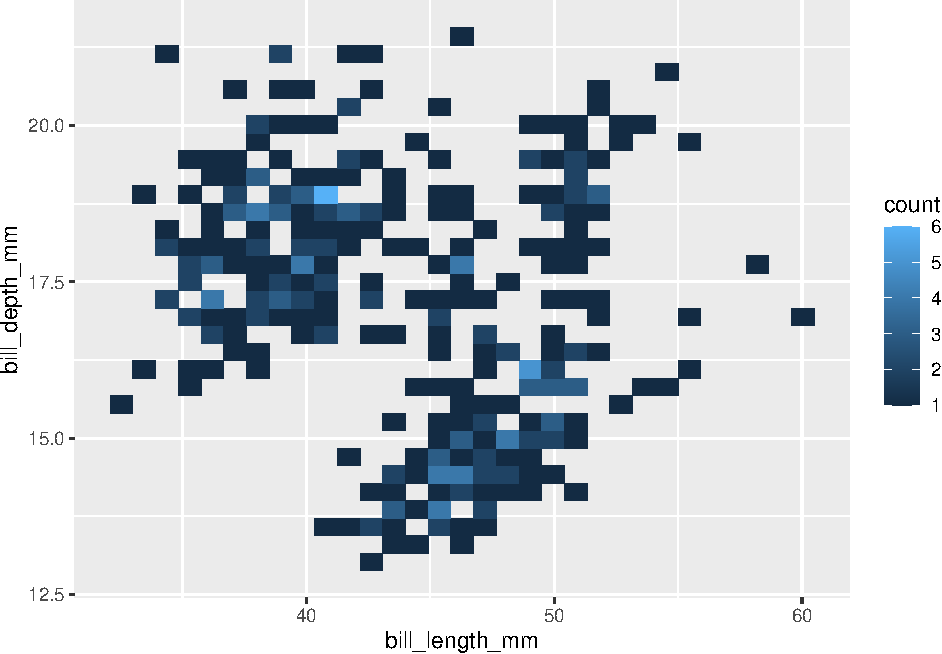
\includegraphics{bookdown-demo_files/figure-latex/unnamed-chunk-193-1.pdf}

\hypertarget{personalizaciuxf3n-de-gruxe1ficos-1}{%
\section{Personalización de gráficos}\label{personalizaciuxf3n-de-gruxe1ficos-1}}

Ahora, personalizaremos el gráfico cambiando colores y añadiendo una línea de tendencia.

\begin{Shaded}
\begin{Highlighting}[]
\FunctionTok{ggplot}\NormalTok{(}\AttributeTok{data =}\NormalTok{ mtcars, }\FunctionTok{aes}\NormalTok{(}\AttributeTok{x =}\NormalTok{ wt, }\AttributeTok{y =}\NormalTok{ mpg, }\AttributeTok{color =} \FunctionTok{factor}\NormalTok{(gear))) }\SpecialCharTok{+} 
  \FunctionTok{geom\_point}\NormalTok{() }\SpecialCharTok{+}
  \FunctionTok{geom\_smooth}\NormalTok{(}\AttributeTok{method =} \StringTok{"lm"}\NormalTok{, }\AttributeTok{se =} \ConstantTok{FALSE}\NormalTok{) }\SpecialCharTok{+}
  \FunctionTok{labs}\NormalTok{(}\AttributeTok{title =} \StringTok{"Consumo de Gasolina vs. Peso por Tipo de Cambio"}\NormalTok{,}
       \AttributeTok{x =} \StringTok{"Peso (1000 lbs)"}\NormalTok{,}
       \AttributeTok{y =} \StringTok{"Millas por Galón (mpg)"}\NormalTok{,}
       \AttributeTok{color =} \StringTok{"Tipo de Cambio"}\NormalTok{) }\SpecialCharTok{+}
  \FunctionTok{theme\_minimal}\NormalTok{()}
\end{Highlighting}
\end{Shaded}

\begin{verbatim}
## `geom_smooth()` using formula = 'y ~ x'
\end{verbatim}

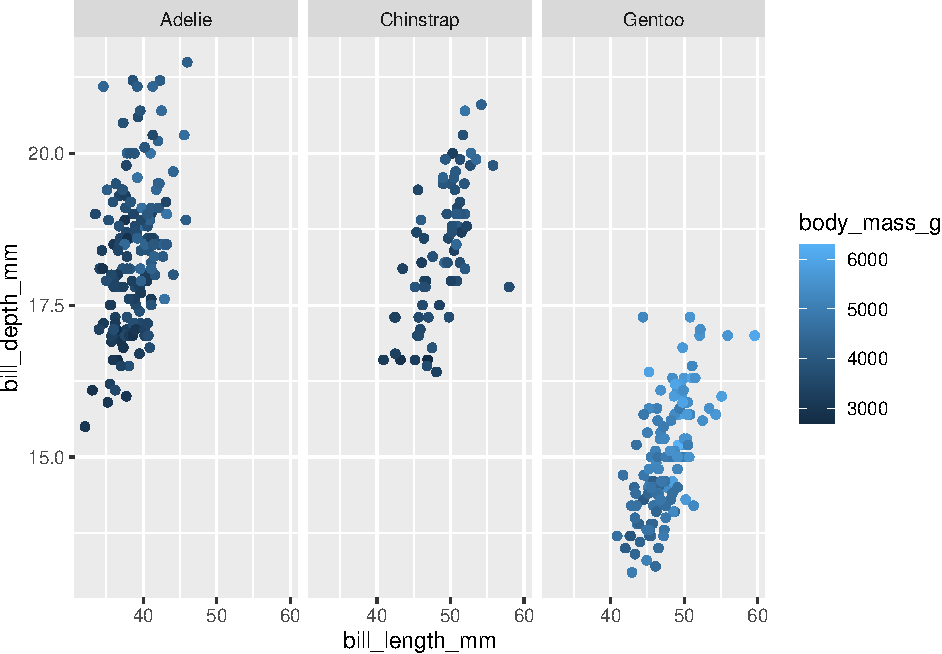
\includegraphics{bookdown-demo_files/figure-latex/unnamed-chunk-194-1.pdf}
\#\#\# Ejercicios sugeridos

\begin{enumerate}
\def\labelenumi{\arabic{enumi}.}
\tightlist
\item
  Explora otro conjunto de datos: Utiliza el conjunto de datos iris para crear un gráfico de dispersión que muestre la relación entre Sepal.Length y Sepal.Width. Colorea los puntos según la especie.
\item
  Personaliza tu gráfico: Añade títulos personalizados a los ejes y al gráfico. Experimenta con diferentes temas, como theme\_bw() o theme\_light().
\item
  Exploración de geométricas: Utiliza geom\_histogram() para crear un histograma del Sepal.Length en el conjunto de datos iris. Ajusta los parámetros binwidth y fill.
\item
  Facetas para múltiples gráficos: Utiliza facet\_wrap(\textasciitilde{} species) para crear gráficos separados para cada especie en el conjunto de datos iris, mostrando la relación entre Sepal.Length y Sepal.Width.
\end{enumerate}

\hypertarget{soluciones-a-los-ejercicios-sugeridos-1}{%
\section{Soluciones a los ejercicios sugeridos}\label{soluciones-a-los-ejercicios-sugeridos-1}}

\begin{Shaded}
\begin{Highlighting}[]
\FunctionTok{ggplot}\NormalTok{(}\AttributeTok{data =}\NormalTok{ iris, }\FunctionTok{aes}\NormalTok{(}\AttributeTok{x =}\NormalTok{ Sepal.Length, }\AttributeTok{y =}\NormalTok{ Sepal.Width, }\AttributeTok{color =}\NormalTok{ Species)) }\SpecialCharTok{+} 
  \FunctionTok{geom\_point}\NormalTok{() }\SpecialCharTok{+}
  \FunctionTok{labs}\NormalTok{(}\AttributeTok{title =} \StringTok{"Relación entre el Largo y el Ancho del Sépalo por Especie"}\NormalTok{,}
       \AttributeTok{x =} \StringTok{"Largo del Sépalo"}\NormalTok{,}
       \AttributeTok{y =} \StringTok{"Ancho del Sépalo"}\NormalTok{)}
\end{Highlighting}
\end{Shaded}

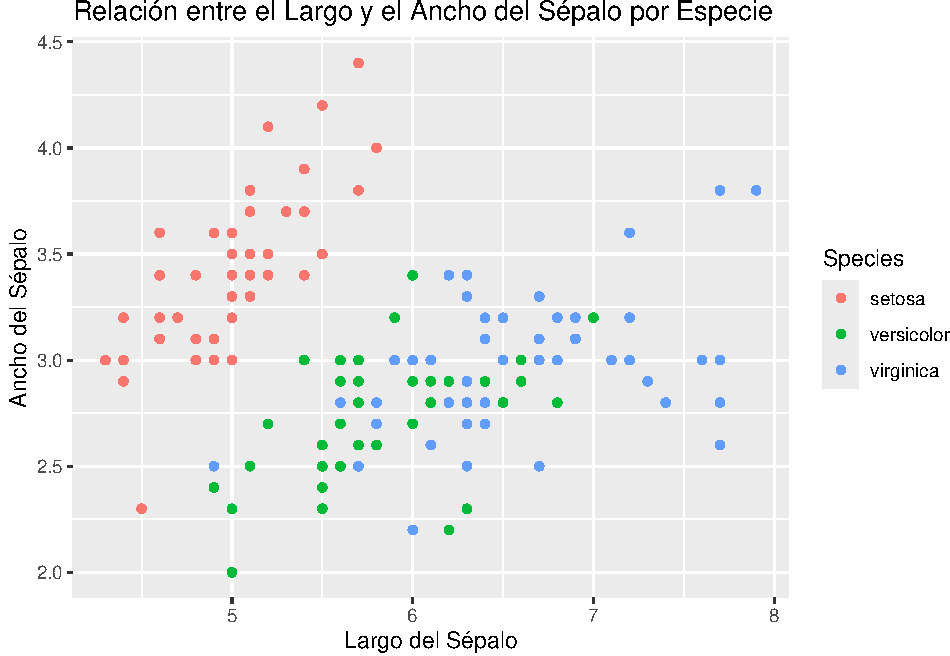
\includegraphics{bookdown-demo_files/figure-latex/unnamed-chunk-195-1.pdf}

\begin{Shaded}
\begin{Highlighting}[]
\FunctionTok{ggplot}\NormalTok{(}\AttributeTok{data =}\NormalTok{ iris, }\FunctionTok{aes}\NormalTok{(}\AttributeTok{x =}\NormalTok{ Sepal.Length, }\AttributeTok{y =}\NormalTok{ Sepal.Width, }\AttributeTok{color =}\NormalTok{ Species)) }\SpecialCharTok{+} 
  \FunctionTok{geom\_point}\NormalTok{() }\SpecialCharTok{+}
  \FunctionTok{labs}\NormalTok{(}\AttributeTok{title =} \StringTok{"Relación entre el Largo y el Ancho del Sépalo por Especie"}\NormalTok{,}
       \AttributeTok{x =} \StringTok{"Largo del Sépalo"}\NormalTok{,}
       \AttributeTok{y =} \StringTok{"Ancho del Sépalo"}\NormalTok{) }\SpecialCharTok{+}
  \FunctionTok{theme\_light}\NormalTok{() }\SpecialCharTok{+}
  \FunctionTok{theme}\NormalTok{(}\AttributeTok{legend.title =} \FunctionTok{element\_blank}\NormalTok{())}
\end{Highlighting}
\end{Shaded}

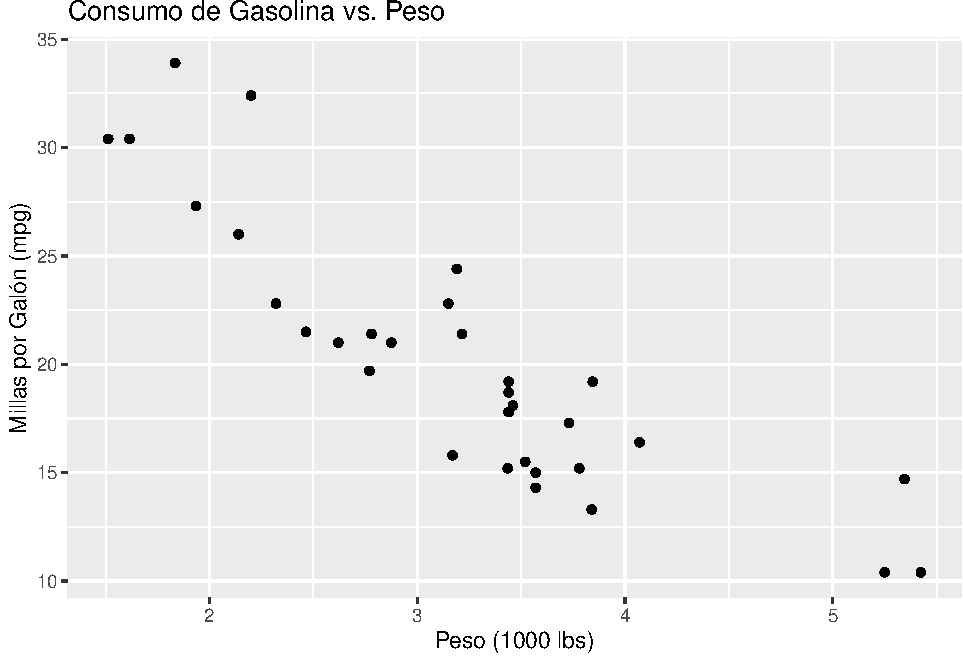
\includegraphics{bookdown-demo_files/figure-latex/unnamed-chunk-196-1.pdf}

\begin{Shaded}
\begin{Highlighting}[]
\FunctionTok{ggplot}\NormalTok{(}\AttributeTok{data =}\NormalTok{ iris, }\FunctionTok{aes}\NormalTok{(}\AttributeTok{x =}\NormalTok{ Sepal.Length)) }\SpecialCharTok{+} 
  \FunctionTok{geom\_histogram}\NormalTok{(}\AttributeTok{binwidth =} \FloatTok{0.5}\NormalTok{, }\AttributeTok{fill =} \StringTok{"blue"}\NormalTok{) }\SpecialCharTok{+}
  \FunctionTok{labs}\NormalTok{(}\AttributeTok{title =} \StringTok{"Distribución del Largo del Sépalo"}\NormalTok{,}
       \AttributeTok{x =} \StringTok{"Largo del Sépalo"}\NormalTok{,}
       \AttributeTok{y =} \StringTok{"Frecuencia"}\NormalTok{)}
\end{Highlighting}
\end{Shaded}

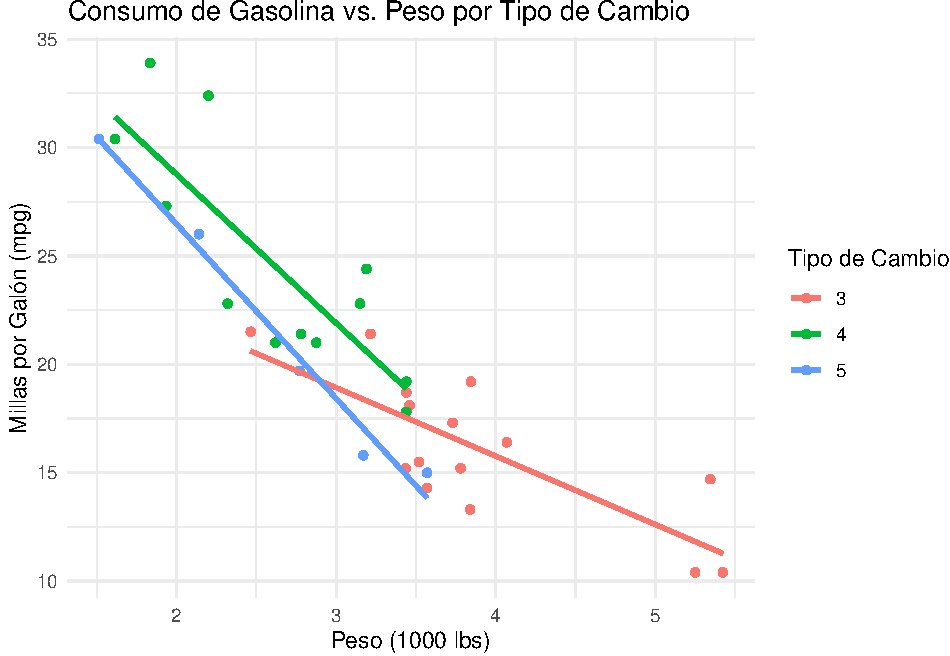
\includegraphics{bookdown-demo_files/figure-latex/unnamed-chunk-197-1.pdf}

\begin{Shaded}
\begin{Highlighting}[]
\FunctionTok{ggplot}\NormalTok{(}\AttributeTok{data =}\NormalTok{ iris, }\FunctionTok{aes}\NormalTok{(}\AttributeTok{x =}\NormalTok{ Sepal.Length, }\AttributeTok{y =}\NormalTok{ Sepal.Width)) }\SpecialCharTok{+} 
  \FunctionTok{geom\_point}\NormalTok{() }\SpecialCharTok{+}
  \FunctionTok{facet\_wrap}\NormalTok{(}\SpecialCharTok{\textasciitilde{}}\NormalTok{ Species) }\SpecialCharTok{+}
  \FunctionTok{labs}\NormalTok{(}\AttributeTok{title =} \StringTok{"Relación entre el Largo y el Ancho del Sépalo por Especie"}\NormalTok{,}
       \AttributeTok{x =} \StringTok{"Largo del Sépalo"}\NormalTok{,}
       \AttributeTok{y =} \StringTok{"Ancho del Sépalo"}\NormalTok{)}
\end{Highlighting}
\end{Shaded}

\includegraphics{bookdown-demo_files/figure-latex/unnamed-chunk-198-1.pdf}

\hypertarget{ejercicios-resueltos-1}{%
\section{Ejercicios resueltos}\label{ejercicios-resueltos-1}}

En esta sección usaremos la librería \texttt{palmerpenguins}

\begin{Shaded}
\begin{Highlighting}[]
\FunctionTok{library}\NormalTok{(palmerpenguins)}
\FunctionTok{library}\NormalTok{(ggplot2)}
\end{Highlighting}
\end{Shaded}

\hypertarget{ejercicio-1-gruxe1fico-de-dispersiuxf3n-buxe1sico-1}{%
\subsection{Ejercicio 1: Gráfico de dispersión básico}\label{ejercicio-1-gruxe1fico-de-dispersiuxf3n-buxe1sico-1}}

Crea un gráfico de dispersión para visualizar la relación entre la longitud del culmen y la profundidad del culmen de los pingüinos.

\begin{Shaded}
\begin{Highlighting}[]
\FunctionTok{ggplot}\NormalTok{(penguins, }\FunctionTok{aes}\NormalTok{(}\AttributeTok{x =}\NormalTok{ bill\_length\_mm, }\AttributeTok{y =}\NormalTok{ bill\_depth\_mm)) }\SpecialCharTok{+}
  \FunctionTok{geom\_point}\NormalTok{()}
\end{Highlighting}
\end{Shaded}

\begin{verbatim}
## Warning: Removed 2 rows containing missing values or values outside the scale range
## (`geom_point()`).
\end{verbatim}

\includegraphics{bookdown-demo_files/figure-latex/unnamed-chunk-200-1.pdf}

\hypertarget{ejercicio-2-diferenciaciuxf3n-por-especie-1}{%
\subsection{Ejercicio 2: Diferenciación por especie}\label{ejercicio-2-diferenciaciuxf3n-por-especie-1}}

Modifica el gráfico de dispersión anterior para diferenciar los puntos por especie de pingüino.

\begin{Shaded}
\begin{Highlighting}[]
\FunctionTok{ggplot}\NormalTok{(penguins, }\FunctionTok{aes}\NormalTok{(}\AttributeTok{x =}\NormalTok{ bill\_length\_mm, }\AttributeTok{y =}\NormalTok{ bill\_depth\_mm, }\AttributeTok{color =}\NormalTok{ species)) }\SpecialCharTok{+}
  \FunctionTok{geom\_point}\NormalTok{()}
\end{Highlighting}
\end{Shaded}

\begin{verbatim}
## Warning: Removed 2 rows containing missing values or values outside the scale range
## (`geom_point()`).
\end{verbatim}

\includegraphics{bookdown-demo_files/figure-latex/unnamed-chunk-201-1.pdf}

\hypertarget{ejercicio-3-histograma-de-masa-corporal-1}{%
\subsection{Ejercicio 3: Histograma de masa corporal}\label{ejercicio-3-histograma-de-masa-corporal-1}}

Crea un histograma para explorar la distribución de la masa corporal de los pingüinos.

\begin{Shaded}
\begin{Highlighting}[]
\FunctionTok{ggplot}\NormalTok{(penguins, }\FunctionTok{aes}\NormalTok{(}\AttributeTok{x =}\NormalTok{ body\_mass\_g)) }\SpecialCharTok{+}
  \FunctionTok{geom\_histogram}\NormalTok{(}\AttributeTok{bins =} \DecValTok{30}\NormalTok{)}
\end{Highlighting}
\end{Shaded}

\begin{verbatim}
## Warning: Removed 2 rows containing non-finite outside the scale range
## (`stat_bin()`).
\end{verbatim}

\includegraphics{bookdown-demo_files/figure-latex/unnamed-chunk-202-1.pdf}

\hypertarget{ejercicio-4-barras-de-error-por-especie-1}{%
\subsection{Ejercicio 4: Barras de error por especie}\label{ejercicio-4-barras-de-error-por-especie-1}}

Genera un gráfico de barras que muestre la masa corporal media de los pingüinos por especie, incluyendo barras de error.

\begin{Shaded}
\begin{Highlighting}[]
\FunctionTok{ggplot}\NormalTok{(penguins, }\FunctionTok{aes}\NormalTok{(}\AttributeTok{x =}\NormalTok{ species, }\AttributeTok{y =}\NormalTok{ body\_mass\_g)) }\SpecialCharTok{+}
  \FunctionTok{geom\_bar}\NormalTok{(}\AttributeTok{stat =} \StringTok{"summary"}\NormalTok{, }\AttributeTok{fun =} \StringTok{"mean"}\NormalTok{) }\SpecialCharTok{+}
  \FunctionTok{geom\_errorbar}\NormalTok{(}\AttributeTok{stat =} \StringTok{"summary"}\NormalTok{, }\AttributeTok{fun.data =}\NormalTok{ mean\_se, }\AttributeTok{width =} \FloatTok{0.2}\NormalTok{)}
\end{Highlighting}
\end{Shaded}

\begin{verbatim}
## Warning: Removed 2 rows containing non-finite outside the scale range
## (`stat_summary()`).
## Removed 2 rows containing non-finite outside the scale range
## (`stat_summary()`).
\end{verbatim}

\includegraphics{bookdown-demo_files/figure-latex/unnamed-chunk-203-1.pdf}

\#\#\#Ejercicio 5: Boxplot de profundidad del culmen
Crea un boxplot para comparar la profundidad del culmen entre las diferentes especies de pingüinos.

\begin{Shaded}
\begin{Highlighting}[]
\FunctionTok{ggplot}\NormalTok{(penguins, }\FunctionTok{aes}\NormalTok{(}\AttributeTok{x =}\NormalTok{ species, }\AttributeTok{y =}\NormalTok{ bill\_depth\_mm)) }\SpecialCharTok{+}
  \FunctionTok{geom\_boxplot}\NormalTok{()}
\end{Highlighting}
\end{Shaded}

\begin{verbatim}
## Warning: Removed 2 rows containing non-finite outside the scale range
## (`stat_boxplot()`).
\end{verbatim}

\includegraphics{bookdown-demo_files/figure-latex/unnamed-chunk-204-1.pdf}

\hypertarget{ejercicio-6-facetado-por-islas-1}{%
\subsection{Ejercicio 6: Facetado por islas}\label{ejercicio-6-facetado-por-islas-1}}

Repite el gráfico de dispersión de longitud vs.~profundidad del culmen, pero esta vez facetado por la isla de origen.

\begin{Shaded}
\begin{Highlighting}[]
\FunctionTok{ggplot}\NormalTok{(penguins, }\FunctionTok{aes}\NormalTok{(}\AttributeTok{x =}\NormalTok{ bill\_length\_mm, }\AttributeTok{y =}\NormalTok{ bill\_depth\_mm)) }\SpecialCharTok{+}
  \FunctionTok{geom\_point}\NormalTok{() }\SpecialCharTok{+}
  \FunctionTok{facet\_wrap}\NormalTok{(}\SpecialCharTok{\textasciitilde{}}\NormalTok{island)}
\end{Highlighting}
\end{Shaded}

\begin{verbatim}
## Warning: Removed 2 rows containing missing values or values outside the scale range
## (`geom_point()`).
\end{verbatim}

\includegraphics{bookdown-demo_files/figure-latex/unnamed-chunk-205-1.pdf}

\hypertarget{ejercicio-7-densidad-de-masa-corporal-1}{%
\subsection{Ejercicio 7: Densidad de masa corporal}\label{ejercicio-7-densidad-de-masa-corporal-1}}

Muestra la densidad de la distribución de la masa corporal de los pingüinos utilizando un gráfico de densidad.

\begin{Shaded}
\begin{Highlighting}[]
\FunctionTok{ggplot}\NormalTok{(penguins, }\FunctionTok{aes}\NormalTok{(}\AttributeTok{x =}\NormalTok{ body\_mass\_g, }\AttributeTok{fill =}\NormalTok{ species)) }\SpecialCharTok{+}
  \FunctionTok{geom\_density}\NormalTok{(}\AttributeTok{alpha =} \FloatTok{0.7}\NormalTok{)}
\end{Highlighting}
\end{Shaded}

\begin{verbatim}
## Warning: Removed 2 rows containing non-finite outside the scale range
## (`stat_density()`).
\end{verbatim}

\includegraphics{bookdown-demo_files/figure-latex/unnamed-chunk-206-1.pdf}

\hypertarget{ejercicio-8-gruxe1fico-de-violuxedn-de-la-longitud-del-culmen-1}{%
\subsection{Ejercicio 8: Gráfico de violín de la longitud del culmen}\label{ejercicio-8-gruxe1fico-de-violuxedn-de-la-longitud-del-culmen-1}}

Genera un gráfico de violín para visualizar la distribución de la longitud del culmen por especie.

\begin{Shaded}
\begin{Highlighting}[]
\FunctionTok{ggplot}\NormalTok{(penguins, }\FunctionTok{aes}\NormalTok{(}\AttributeTok{x =}\NormalTok{ species, }\AttributeTok{y =}\NormalTok{ bill\_length\_mm)) }\SpecialCharTok{+}
  \FunctionTok{geom\_violin}\NormalTok{()}
\end{Highlighting}
\end{Shaded}

\begin{verbatim}
## Warning: Removed 2 rows containing non-finite outside the scale range
## (`stat_ydensity()`).
\end{verbatim}

\includegraphics{bookdown-demo_files/figure-latex/unnamed-chunk-207-1.pdf}

\hypertarget{ejercicio-9-puntos-superpuestos-en-boxplot-1}{%
\subsection{Ejercicio 9: Puntos superpuestos en boxplot}\label{ejercicio-9-puntos-superpuestos-en-boxplot-1}}

Crea un boxplot de la profundidad del culmen por especie y superpón los puntos de datos individuales.

\begin{Shaded}
\begin{Highlighting}[]
\FunctionTok{ggplot}\NormalTok{(penguins, }\FunctionTok{aes}\NormalTok{(}\AttributeTok{x =}\NormalTok{ species, }\AttributeTok{y =}\NormalTok{ bill\_depth\_mm)) }\SpecialCharTok{+}
  \FunctionTok{geom\_boxplot}\NormalTok{(}\AttributeTok{alpha =} \FloatTok{0.5}\NormalTok{) }\SpecialCharTok{+}
  \FunctionTok{geom\_jitter}\NormalTok{(}\AttributeTok{width =} \FloatTok{0.2}\NormalTok{)}
\end{Highlighting}
\end{Shaded}

\begin{verbatim}
## Warning: Removed 2 rows containing non-finite outside the scale range
## (`stat_boxplot()`).
\end{verbatim}

\begin{verbatim}
## Warning: Removed 2 rows containing missing values or values outside the scale range
## (`geom_point()`).
\end{verbatim}

\includegraphics{bookdown-demo_files/figure-latex/unnamed-chunk-208-1.pdf}

\hypertarget{ejercicio-10-gruxe1fico-de-luxedneas-de-masa-corporal-promedio-a-lo-largo-del-tiempo-1}{%
\subsection{Ejercicio 10: Gráfico de líneas de masa corporal promedio a lo largo del tiempo}\label{ejercicio-10-gruxe1fico-de-luxedneas-de-masa-corporal-promedio-a-lo-largo-del-tiempo-1}}

Asumiendo que los datos estén ordenados temporalmente, muestra cómo cambia la masa corporal promedio a lo largo del tiempo.

\begin{Shaded}
\begin{Highlighting}[]
\CommentTok{\# Asumiendo que \textquotesingle{}year\textquotesingle{} representa el tiempo en tus datos}
\FunctionTok{ggplot}\NormalTok{(penguins, }\FunctionTok{aes}\NormalTok{(}\AttributeTok{x =}\NormalTok{ year, }\AttributeTok{y =}\NormalTok{ body\_mass\_g, }\AttributeTok{group =} \DecValTok{1}\NormalTok{)) }\SpecialCharTok{+}
  \FunctionTok{geom\_line}\NormalTok{(}\AttributeTok{stat =} \StringTok{"summary"}\NormalTok{, }\AttributeTok{fun =} \StringTok{"mean"}\NormalTok{)}
\end{Highlighting}
\end{Shaded}

\begin{verbatim}
## Warning: Removed 2 rows containing non-finite outside the scale range
## (`stat_summary()`).
\end{verbatim}

\includegraphics{bookdown-demo_files/figure-latex/unnamed-chunk-209-1.pdf}

\hypertarget{ejercicio-11-gruxe1fico-de-dispersiuxf3n-con-tamauxf1o-de-punto-1}{%
\subsection{Ejercicio 11: Gráfico de dispersión con tamaño de punto}\label{ejercicio-11-gruxe1fico-de-dispersiuxf3n-con-tamauxf1o-de-punto-1}}

Modifica el gráfico de dispersión de longitud vs.~profundidad del culmen para que el tamaño de los puntos refleje la masa corporal de los pingüinos.

\begin{Shaded}
\begin{Highlighting}[]
\FunctionTok{ggplot}\NormalTok{(penguins, }\FunctionTok{aes}\NormalTok{(}\AttributeTok{x =}\NormalTok{ bill\_length\_mm, }\AttributeTok{y =}\NormalTok{ bill\_depth\_mm, }\AttributeTok{size =}\NormalTok{ body\_mass\_g)) }\SpecialCharTok{+}
  \FunctionTok{geom\_point}\NormalTok{(}\AttributeTok{alpha =} \FloatTok{0.5}\NormalTok{)}
\end{Highlighting}
\end{Shaded}

\begin{verbatim}
## Warning: Removed 2 rows containing missing values or values outside the scale range
## (`geom_point()`).
\end{verbatim}

\includegraphics{bookdown-demo_files/figure-latex/unnamed-chunk-210-1.pdf}

\hypertarget{ejercicio-12-barras-apiladas-de-especies-por-isla-1}{%
\subsection{Ejercicio 12: Barras apiladas de especies por isla}\label{ejercicio-12-barras-apiladas-de-especies-por-isla-1}}

Crea un gráfico de barras apiladas que muestre la cantidad de pingüinos de cada especie presentes en cada isla.

\begin{Shaded}
\begin{Highlighting}[]
\FunctionTok{ggplot}\NormalTok{(penguins, }\FunctionTok{aes}\NormalTok{(}\AttributeTok{x =}\NormalTok{ island, }\AttributeTok{fill =}\NormalTok{ species)) }\SpecialCharTok{+}
  \FunctionTok{geom\_bar}\NormalTok{(}\AttributeTok{position =} \StringTok{"stack"}\NormalTok{)}
\end{Highlighting}
\end{Shaded}

\includegraphics{bookdown-demo_files/figure-latex/unnamed-chunk-211-1.pdf}

\hypertarget{ejercicio-13-gruxe1fico-de-correlaciuxf3n-con-texto-1}{%
\subsection{Ejercicio 13: Gráfico de correlación con texto}\label{ejercicio-13-gruxe1fico-de-correlaciuxf3n-con-texto-1}}

Genera un gráfico de dispersión entre la longitud y la profundidad del culmen e incluye un texto que muestre el coeficiente de correlación en el gráfico.

\begin{Shaded}
\begin{Highlighting}[]
\FunctionTok{library}\NormalTok{(ggpubr)}
\FunctionTok{ggplot}\NormalTok{(penguins, }\FunctionTok{aes}\NormalTok{(}\AttributeTok{x =}\NormalTok{ bill\_length\_mm, }\AttributeTok{y =}\NormalTok{ bill\_depth\_mm)) }\SpecialCharTok{+}
  \FunctionTok{geom\_point}\NormalTok{() }\SpecialCharTok{+}
  \FunctionTok{stat\_cor}\NormalTok{(}\AttributeTok{method =} \StringTok{"pearson"}\NormalTok{, }\AttributeTok{label.x =} \DecValTok{3}\NormalTok{, }\AttributeTok{label.y =} \DecValTok{50}\NormalTok{)}
\end{Highlighting}
\end{Shaded}

\begin{verbatim}
## Warning: Removed 2 rows containing non-finite outside the scale range
## (`stat_cor()`).
\end{verbatim}

\begin{verbatim}
## Warning: Removed 2 rows containing missing values or values outside the scale range
## (`geom_point()`).
\end{verbatim}

\includegraphics{bookdown-demo_files/figure-latex/unnamed-chunk-212-1.pdf}

\hypertarget{ejercicio-14-mapa-de-calor-de-la-longitud-y-profundidad-del-culmen-1}{%
\subsection{Ejercicio 14: Mapa de calor de la longitud y profundidad del culmen}\label{ejercicio-14-mapa-de-calor-de-la-longitud-y-profundidad-del-culmen-1}}

Crea un mapa de calor que muestre la distribución conjunta de la longitud y la profundidad del culmen de los pingüinos.

\begin{Shaded}
\begin{Highlighting}[]
\FunctionTok{ggplot}\NormalTok{(penguins, }\FunctionTok{aes}\NormalTok{(}\AttributeTok{x =}\NormalTok{ bill\_length\_mm, }\AttributeTok{y =}\NormalTok{ bill\_depth\_mm)) }\SpecialCharTok{+}
  \FunctionTok{geom\_bin2d}\NormalTok{()}
\end{Highlighting}
\end{Shaded}

\begin{verbatim}
## Warning: Removed 2 rows containing non-finite outside the scale range
## (`stat_bin2d()`).
\end{verbatim}

\includegraphics{bookdown-demo_files/figure-latex/unnamed-chunk-213-1.pdf}

\hypertarget{ejercicio-15-gruxe1fico-de-interacciuxf3n-entre-tres-variables-1}{%
\subsection{Ejercicio 15: Gráfico de interacción entre tres variables}\label{ejercicio-15-gruxe1fico-de-interacciuxf3n-entre-tres-variables-1}}

Explora la relación entre la longitud del culmen, la profundidad del culmen y la masa corporal, diferenciando por especie.

\begin{Shaded}
\begin{Highlighting}[]
\FunctionTok{ggplot}\NormalTok{(penguins, }\FunctionTok{aes}\NormalTok{(}\AttributeTok{x =}\NormalTok{ bill\_length\_mm, }\AttributeTok{y =}\NormalTok{ bill\_depth\_mm, }\AttributeTok{color =}\NormalTok{ body\_mass\_g)) }\SpecialCharTok{+}
  \FunctionTok{geom\_point}\NormalTok{() }\SpecialCharTok{+}
  \FunctionTok{facet\_wrap}\NormalTok{(}\SpecialCharTok{\textasciitilde{}}\NormalTok{species)}
\end{Highlighting}
\end{Shaded}

\begin{verbatim}
## Warning: Removed 2 rows containing missing values or values outside the scale range
## (`geom_point()`).
\end{verbatim}

\includegraphics{bookdown-demo_files/figure-latex/unnamed-chunk-214-1.pdf}

\hypertarget{ejercicios-propuestos-1}{%
\subsection{Ejercicios propuestos}\label{ejercicios-propuestos-1}}

\begin{enumerate}
\def\labelenumi{\arabic{enumi}.}
\item
  Gráfico de dispersión con facetas por sexo
  Crea un gráfico de dispersión para examinar la relación entre la longitud del culmen y la profundidad del culmen, separando los datos por sexo de los pingüinos utilizando facetas.
\item
  Comparación de masa corporal entre islas
  Utiliza un gráfico de barras para comparar la masa corporal media de los pingüinos en las diferentes islas.
\item
  Gráfico de densidad por sexo
  Genera gráficos de densidad para la longitud del culmen, diferenciados por sexo de los pingüinos.
\item
  Gráfico de líneas de tendencia para la profundidad del culmen
  Crea un gráfico que muestre la tendencia de la profundidad del culmen a lo largo del tiempo para cada especie de pingüino.
\item
  Mapa de calor de la correlación entre variables numéricas
  Utiliza funciones de \texttt{ggplot2} para crear un mapa de calor que muestre la correlación entre las variables numéricas de los datos de pingüinos.
\item
  Gráfico de barras de conteo por especie
  Crea un gráfico de barras que muestre el número de observaciones (conteo) para cada especie de pingüino.
\item
  Análisis de outliers en la masa corporal
  Utiliza un boxplot para identificar outliers en la masa corporal de los pingüinos y diferencia por especie.
\item
  Gráfico de dispersión con modelado lineal
  Crea un gráfico de dispersión de la longitud vs.~profundidad del culmen e incluye una línea de tendencia lineal.
\item
  Barras apiladas de conteo por isla y especie
  Genera un gráfico de barras apiladas que muestre el número de pingüinos de cada especie en cada isla.
\item
  Gráfico de violín con puntos individuales
  Crea gráficos de violín para la masa corporal de los pingüinos por especie e incluye los puntos individuales de los datos.
\end{enumerate}

\hypertarget{Listas}{%
\chapter{Listas}\label{Listas}}

Las listas son una estructura de datos muy versátil en R, que permiten almacenar una colección de elementos. A diferencia de los vectores, una lista puede contener elementos de diferentes tipos, como números, cadenas y hasta otras listas.

En R, las listas pueden contener una amplia variedad de tipos de datos, incluyendo números, vectores, matrices, y data frames. Esto las hace extremadamente versátiles para la gestión de datos complejos.

\textbf{Ejemplos}

\begin{itemize}
\tightlist
\item
  Creación de una Lista
\end{itemize}

\begin{Shaded}
\begin{Highlighting}[]
\CommentTok{\# Creando una lista con diferentes tipos de datos}
\NormalTok{compleja\_lista }\OtherTok{\textless{}{-}} \FunctionTok{list}\NormalTok{(}
  \AttributeTok{numero =} \DecValTok{42}\NormalTok{,}
  \AttributeTok{vector =} \FunctionTok{c}\NormalTok{(}\DecValTok{1}\NormalTok{, }\DecValTok{2}\NormalTok{, }\DecValTok{3}\NormalTok{),}
  \AttributeTok{matriz =} \FunctionTok{matrix}\NormalTok{(}\FunctionTok{c}\NormalTok{(}\DecValTok{1}\NormalTok{, }\DecValTok{2}\NormalTok{, }\DecValTok{3}\NormalTok{, }\DecValTok{4}\NormalTok{), }\AttributeTok{nrow =} \DecValTok{2}\NormalTok{),}
  \AttributeTok{data\_frame =} \FunctionTok{data.frame}\NormalTok{(}\AttributeTok{nombre =} \FunctionTok{c}\NormalTok{(}\StringTok{"E. coli"}\NormalTok{, }\StringTok{"S. aureus"}\NormalTok{), }\AttributeTok{gram =} \FunctionTok{c}\NormalTok{(}\StringTok{"+"}\NormalTok{, }\StringTok{"{-}"}\NormalTok{))}
\NormalTok{)}

\FunctionTok{print}\NormalTok{(compleja\_lista)}
\end{Highlighting}
\end{Shaded}

\begin{verbatim}
## $numero
## [1] 42
## 
## $vector
## [1] 1 2 3
## 
## $matriz
##      [,1] [,2]
## [1,]    1    3
## [2,]    2    4
## 
## $data_frame
##      nombre gram
## 1   E. coli    +
## 2 S. aureus    -
\end{verbatim}

Para acceder a los elementos de una lista, puedes usar el doble corchete {[}{[} {]}{]} o el operador de dólar \$. El doble corchete es útil para acceder a los elementos por su índice, mientras que el operador de dólar se usa con nombres.

Accceso por índice

\begin{Shaded}
\begin{Highlighting}[]
\CommentTok{\# Accediendo al vector dentro de la lista}
\NormalTok{vector\_en\_lista }\OtherTok{\textless{}{-}}\NormalTok{ compleja\_lista[[}\DecValTok{2}\NormalTok{]]}
\FunctionTok{print}\NormalTok{(vector\_en\_lista)}
\end{Highlighting}
\end{Shaded}

\begin{verbatim}
## [1] 1 2 3
\end{verbatim}

\hypertarget{acceso-por-nombre}{%
\subsection{Acceso por Nombre}\label{acceso-por-nombre}}

\begin{Shaded}
\begin{Highlighting}[]
\CommentTok{\# Accediendo al data frame por nombre}
\NormalTok{data\_frame\_en\_lista }\OtherTok{\textless{}{-}}\NormalTok{ compleja\_lista}\SpecialCharTok{$}\NormalTok{data\_frame}
\FunctionTok{print}\NormalTok{(data\_frame\_en\_lista)}
\end{Highlighting}
\end{Shaded}

\begin{verbatim}
##      nombre gram
## 1   E. coli    +
## 2 S. aureus    -
\end{verbatim}

\hypertarget{ejercicios-3}{%
\section{Ejercicios}\label{ejercicios-3}}

\hypertarget{ejercicios-propuestos-con-listas}{%
\subsection{Ejercicios Propuestos con listas}\label{ejercicios-propuestos-con-listas}}

\begin{enumerate}
\def\labelenumi{\arabic{enumi}.}
\item
  Crea una lista que contenga al menos cuatro tipos diferentes de datos (incluyendo al menos un vector, una matriz, y un data frame). Luego, escribe código para acceder a cada uno de estos elementos por su índice.
\item
  Añade un nuevo elemento a la compleja\_lista que sea otra lista conteniendo información relevante a un experimento microbiológico (p.ej., fechas, resultados de crecimiento, tipo de medio de cultivo). Accede a un elemento específico dentro de esta lista anidada.
\end{enumerate}

Recuerda, el uso efectivo de listas en R puede ayudarte a gestionar y manipular una amplia gama de conjuntos de datos complejos, especialmente útil en campos como la Microbiología.

\hypertarget{referencias}{%
\chapter{Referencias}\label{referencias}}

  \bibliography{book.bib}

\end{document}
